%% Compile pdflatex > biber > pdflatex > pdflatex, or: latexmk -pdf thesisv2
%% Set \workingdocfalse before final submission to hide 
\newif\ifworkingdoc
\workingdocfalse

\documentclass[11pt,a4paper]{article}

\usepackage[utf8]{inputenc}
\usepackage[T1]{fontenc}
\usepackage{textcomp}
\usepackage{lmodern}
\usepackage[british]{babel}

\usepackage[
  a4paper,
  top    = 2.5cm,
  bottom = 2.5cm,
  left   = 3.0cm,
  right  = 2.5cm,
]{geometry}

\usepackage{setspace}
\onehalfspacing
\setlength{\parindent}{0pt}
\setlength{\parskip}{6pt plus 2pt minus 1pt}

\usepackage{csquotes}
\usepackage[
  backend = biber,
  style   = apa,
  sorting = nyt,
  natbib  = true,
]{biblatex}
\DeclareLanguageMapping{british}{british-apa}
\addbibresource{bibliography.bib}

\usepackage{amsmath,amssymb}
\usepackage{bm}

\usepackage{booktabs}
\usepackage{longtable}
\usepackage{tabularx}
\usepackage{array}
\usepackage{multirow}
\usepackage{graphicx}
\usepackage{float}
\usepackage{rotating}
\usepackage{pdflscape}
\usepackage{enumitem}

\usepackage{tikz}
\usetikzlibrary{positioning, arrows, calc, shapes.geometric, shapes.misc,
  fit, backgrounds, decorations.pathmorphing, decorations.pathreplacing,
  shadows, chains, matrix}

\definecolor{thesisNavy}{HTML}{1F3A5F}
\definecolor{thesisTeal}{HTML}{2A7F8C}
\definecolor{thesisOrange}{HTML}{D97706}
\definecolor{thesisRed}{HTML}{C44536}
\definecolor{thesisGreen}{HTML}{4A7C59}
\definecolor{thesisGrey}{HTML}{6B7280}
\definecolor{thesisLight}{HTML}{F3F4F6}
\definecolor{thesisMid}{HTML}{D1D5DB}

\tikzset{
  thesis stage/.style={
    draw=thesisNavy, line width=0.8pt, rounded corners=3pt,
    fill=thesisLight, minimum width=2.7cm, minimum height=1.5cm,
    align=center, font=\small, drop shadow={shadow xshift=1pt,
    shadow yshift=-1pt, opacity=0.15}
  },
  thesis alloc/.style={
    draw=thesisTeal, line width=0.8pt, rounded corners=3pt,
    fill=thesisTeal!10, minimum width=2.2cm, minimum height=1.5cm,
    align=center, font=\small, drop shadow={shadow xshift=1pt,
    shadow yshift=-1pt, opacity=0.15}
  },
  thesis arrow/.style={-latex, draw=thesisNavy, line width=0.8pt},
  thesis dashedbox/.style={
    draw=thesisGrey, dashed, rounded corners=6pt, line width=0.6pt,
    inner sep=12pt
  },
  thesis factor/.style={
    draw=thesisOrange, line width=0.5pt, fill=thesisOrange!10,
    rounded corners=2pt, inner sep=2pt, font=\scriptsize,
    text=thesisOrange!70!black
  },
  fcell0/.style={fill=thesisLight, draw=thesisGrey!60, line width=0.25pt},
  fcell1/.style={fill=thesisOrange!70, draw=thesisGrey!60, line width=0.25pt},
}

\newcolumntype{L}[1]{>{\raggedright\arraybackslash}p{#1}}
\newcolumntype{C}[1]{>{\centering\arraybackslash}p{#1}}

\usepackage[font=small, labelfont=bf, skip=4pt]{caption}

\usepackage{xcolor}

\usepackage[
  colorlinks        = true,
  linkcolor         = blue!60!black,
  citecolor         = blue!60!black,
  urlcolor          = blue!60!black,
  pdftitle          = {Decomposition of Global Minimum Tax Revenue Using CbCR Data},
  pdfauthor         = {Maurits de Haan},
  pdfsubject        = {MSc Economic Policy Thesis - Utrecht University},
  pdfkeywords       = {global minimum tax; Pillar Two; CbCR; revenue estimation; ETR; profit shifting; BEPS},
  pdfstartview      = FitH,
  bookmarksopen     = true,
  bookmarksnumbered = true,
]{hyperref}

\usepackage[colorinlistoftodos]{todonotes}

\usepackage{titlesec}
\titleformat{\section}{\large\bfseries}{\thesection}{1em}{}
\titleformat{\subsection}{\normalsize\bfseries}{\thesubsection}{1em}{}
\titleformat{\subsubsection}{\normalsize\itshape}{\thesubsubsection}{1em}{}

\makeatletter
\renewcommand{\l@section}{\@dottedtocline{1}{0em}{2.8em}}
\renewcommand{\l@subsection}{\@dottedtocline{2}{2.8em}{3.6em}}
\renewcommand{\l@subsubsection}{\@dottedtocline{3}{6.4em}{4.2em}}
\makeatother

\usepackage{fancyhdr}
\pagestyle{fancy}
\fancyhf{}
\fancyhead[L]{\small\itshape\leftmark}
\fancyhead[R]{\small\itshape de Haan (\the\year)}
\fancyfoot[C]{\small\thepage}
\renewcommand{\headrulewidth}{0.4pt}
\renewcommand{\footrulewidth}{0pt}

\fancypagestyle{plain}{%
  \fancyhf{}
  \fancyfoot[C]{\small\thepage}
  \renewcommand{\headrulewidth}{0pt}
}

%% Toggle: \workingdoctrue / \workingdocfalse (set at top of file)
%% When false, \workingnote{...} produces no output.
\newcommand{\workingnote}[1]{\ifworkingdoc{\textcolor{red}{\textit{[Working note: #1]}}}\fi}

\newcommand{\GMT}{GMT}
\newcommand{\GloBE}{GloBE}
\newcommand{\ETR}{ETR}
\newcommand{\SBIE}{SBIE}
\newcommand{\IIR}{IIR}
\newcommand{\UTPR}{UTPR}
\newcommand{\STTR}{STTR}
\newcommand{\CbCR}{CbCR}
\newcommand{\MNE}{MNE}
\newcommand{\pp}{\text{pp}}
\newcommand{\EUR}{\texteuro}
\newcommand{\code}[1]{\texttt{#1}}
\newcommand{\assumption}[2]{\noindent\textbf{Assumption #1.} \textit{#2}\medskip}

\begin{document}


\begin{titlepage}
  \thispagestyle{empty}
  \begin{center}

    \vspace*{1.5em}
    {\large\bfseries Utrecht University School of Economics}\\[0.3em]

    
\includegraphics[height=2.5cm]{UU_logo_2021_EN_RGB.png}\\[0.8em]

    \rule{\textwidth}{1pt}\\[1.2em]

    {\LARGE\bfseries
      Decomposition of Global Minimum Tax\\[0.3em]
      revenue using CbCR data:%
      \footnote{The copyright of this thesis rests with the author. The author is responsible for its contents and opinions expressed in the thesis. U.S.E.\ is only responsible for the academic coaching and supervision and cannot be held liable for the content. I am grateful to dr. Peter Gerbrands for valuable comments and discussions. \workingnote{check that this is compliant with UU rules}}}%
    \\[1.2em]

    \rule{\textwidth}{1pt}\\[2.5em]

    {\large Maurits de Haan}\\[0.3em]
    {\normalsize\href{mailto:m.c.p.dehaan@students.uu.nl}
      {m.c.p.dehaan@students.uu.nl}}\\
    {\normalsize\href{mailto:maurits.cpdehaan@gmail.com}
      {maurits.cpdehaan@gmail.com}}\\[2.5em]

    \begin{tabular}{@{}rl@{}}
      \textbf{Supervisor:} & dr.\ Peter Gerbrands \\[0.4em]
      \textbf{Second reader:} & dr.\ Adriaan Kalwij \\[0.4em]
      \textbf{Programme:} & MSc Economic Policy \\[0.4em]
      \textbf{University:} & Utrecht University \\[0.4em]
      \textbf{Academic year:} & 2025--2026 \\[0.4em]
      \textbf{Date last updated:} & \today \\
    \end{tabular}

    \vfill

    \begin{tabular}{@{}ll@{}}
      \textbf{JEL codes:} &
        H25, H26, F23, H87 \\[0.5em]
      \textbf{Keywords:} &
        \parbox[t]{0.75\textwidth}{global minimum tax, Pillar Two,
        country-by-country reporting,\\
        revenue estimation, effective tax rate, profit shifting, BEPS}
    \end{tabular}

  \end{center}
\end{titlepage}

\newpage
\thispagestyle{plain}
\setcounter{page}{1}

\phantomsection
\addcontentsline{toc}{section}{Abstract}
\begin{center}
  {\large\bfseries Abstract}
\end{center}

\noindent

\workingnote{Need to do, at last.}

\newpage

\tableofcontents

\newpage
\listoftables
\listoffigures

\newpage
\phantomsection
\addcontentsline{toc}{section}{List of Abbreviations}
\section*{List of Abbreviations}

\begin{tabular}{@{}ll@{}}
  \toprule
  \textbf{Abbreviation} & \textbf{Definition} \\
  \midrule
  BEA & Bureau of Economic Analysis (US) \\
  BEPS & Base Erosion and Profit Shifting \\
  CbCR & Country-by-Country Reporting \\
  CFC & Controlled Foreign Corporation \\
  CIT & Corporate Income Tax \\
  EATR & Effective Average Tax Rate \\
  EMTR & Effective Marginal Tax Rate \\
  ETR & Effective Tax Rate \\
  EU & European Union \\
  FATS & Foreign Affiliates Statistics \\
  FDI & Foreign Direct Investment \\
  GloBE & Global Anti-Base Erosion (Rules) \\
  GMT & Global Minimum Tax \\
  IIR & Income Inclusion Rule \\
  IP & Intellectual Property \\
  MNE & Multinational Enterprise \\
  NACE & Statistical Classification of Economic Activities (EU) \\
  OECD & Organisation for Economic Co-operation and Development \\
  QDMTT & Qualified Domestic Minimum Top-up Tax \\
  QRTC & Qualified Refundable Tax Credit \\
  SBIE & Substance-Based Income Exclusion \\
  SbS & Side-by-Side (package) \\
  STTR & Subject-to-Tax Rule \\
  TCJA & Tax Cuts and Jobs Act (US, 2017) \\
  UPE & Ultimate Parent Entity \\
  UTPR & Undertaxed Profits Rule \\
  \bottomrule
\end{tabular}

\newpage

\section{Introduction}\label{sec:introduction}

The Global Minimum Tax (GMT) is the most consequential reform of international corporate taxation since the post-war tax treaty network, but the revenue it raises remains poorly understood. Agreed in October 2021 by 137 jurisdictions under the OECD/G20 Inclusive Framework, the GMT imposes a minimum effective tax rate (ETR) of 15\% on profits of multinational enterprises (MNEs) with consolidated revenues above \EUR750 million. Where an affiliate's ETR falls below 15\%, a \emph{top-up tax} closes the gap. The reform responds to four decades of profit shifting estimated at \$300--850 billion annually \citep{torslov2023,garcia-bernardo2024,blouin2023,cobham2018}. By early 2026, more than sixty jurisdictions had enacted GMT legislation. No consensus exists on how much revenue the reform will raise, where it will accrue, or which design features drive the variation.

This thesis produces EU revenue estimates under the GMT and splits the uncertainty into two parts: the statistical precision of the behavioural parameter, which shrinks as more Country-by-Country Reporting (CbCR) data become available, and the scenario spread across reasonable modelling choices, which only further methodological work can close. The split tells finance ministries whether their revenue forecast will move because new data arrive or because a different assumption is adopted.

Revenue estimates of the GMT diverge. \citet{barake2022} compute a global gain of \EUR179 billion on the 2017 CbCR data, of which roughly \EUR55 billion would accrue to the EU. \citet{boukal2026} project a 4.3--5.3\% rise in Slovak corporate tax revenue, with roughly half from new top-up tax and half from reduced profit shifting. However, no study decomposes the sources of divergence or quantifies which assumption drives the largest share of variation.

Three design features of the GMT compound this uncertainty. First, the top-up tax applies only to profit taxed below the 15\% floor, so revenue depends on how within-jurisdiction ETR heterogeneity is measured. \citet{hugger2026} show that 53.2\% of all low-taxed profit sits in jurisdictions whose average ETR exceeds 15\%: estimates based on jurisdiction averages miss more than half the GMT base. Second, the Substance-Based Income Exclusion (SBIE) shields a fraction of profit proportional to payroll and tangible assets, converting the headline 15\% rate into an effective floor that \citet{devereux2023} estimate at only 6.45\% in transition year one for the average in-scope EU subsidiary. Third, the tax semi-elasticity of reported profits is highly nonlinear: \citet{dowd2017} find a profit response six times larger at a 5\% rate than at 30\%, well above the cross-study consensus of 0.8 \citep{heckemeyer2017}.

The magnitude of this behavioural response is governed by the tax semi-elasticity of reported profits: the percentage change in profit reported in a jurisdiction for a one percentage-point change in the tax rate. The consensus estimate of semi-elasticities of 0.8 by \citet{heckemeyer2017} implies that a one percentage-point increase in the tax differential reduces reported profits by 0.8\%. At moderate tax rates this behavioural response is small, but \citet{dowd2017} show that the semi-elasticity rises sharply at low tax rates: at a 5\% statutory rate, a one percentage-point change induces a 4.7\% profit response, nearly six times the consensus estimate. The semi-elasticity is the key parameter that determines how much of the low-taxed profit base survives into the revenue calculation and how much is reallocated before the top-up tax applies.

The top-up tax is collected through three channels in a fixed priority order. A Qualified Domestic Minimum Top-up Tax (QDMTT) allows the source country to collect the top-up itself. Where no QDMTT is in place, the Income Inclusion Rule (IIR) allocates the top-up to the jurisdiction of the ultimate parent entity (UPE). Any residual is collected by affiliate jurisdictions through the Undertaxed Profits Rule (UTPR). The January 2026 OECD Administrative Guidance added two provisions that alter this allocation. The Side-by-Side (SbS) Safe Harbour removes MNE groups headquartered in jurisdictions with a qualifying regime (in practice, the United States) from IIR and UTPR collection, leaving the QDMTT as the only operative channel for those groups. The Substance-Based Tax Incentive (SBTI) Safe Harbour permits qualifying tax incentives to be added to the GloBE covered tax base up to a cap tied to payroll and tangible assets \citep{oecd2026}. No academic study quantifies their joint revenue consequences.

Finance ministries across the EU budget GMT revenue, calibrate QDMTT parameters, and negotiate SbS terms on the basis of revenue estimates whose sensitivity to modelling assumptions has not been systematically assessed. The Netherlands illustrates the problem. The Dutch government projected \EUR466 million in annual GMT revenue, of which \EUR402 million (86\%) was attributed to the behavioural response: profit that would no longer be shifted to low-tax jurisdictions once the effective floor rises \citep{36369_3}. The revenue projection therefore depends almost entirely on which semi-elasticity is assumed. The SbS package subsequently reduced the Dutch projection by \EUR120 million per year \citep{1028}. A framework that identifies which assumptions drive the largest variation in revenue estimates is therefore relevant to fiscal planning.

The thesis addresses the following research question:

\begin{quote}
\textit{What profit-shifting semi-elasticities emerge from the 2016--2022 CbCR panel under different functional forms, and how sensitive are the resulting Global Minimum Tax revenue estimates for EU Member States to the measurement of effective tax rates, the substance-based income exclusion, the implementation of the Side-by-Side package, and the specification of behavioural responses?}
\end{quote}

Three subquestions structure the analysis:

\begin{enumerate}
\item What profit-shifting semi-elasticities does the 2016--2022 CbCR panel yield when estimated under linear, quadratic, and logarithmic functional forms using the Hines--Rice framework with bilateral fixed effects, and which specification best fits the data?
\item What range of GMT revenue estimates emerges for EU Member States when the panel-estimated semi-elasticities are combined with four further modelling assumptions (ETR measurement, substance exclusion specification, SBIE carve-out rates, and implementation regime) in a full factorial design, and which assumptions and interactions drive the largest share of variation?
\item How do the January 2026 Side-by-Side Safe Harbour and the SBTI Safe Harbour jointly reshape the magnitude and distribution of GMT revenue across EU Member States and across collection channels (QDMTT, IIR, UTPR)?
\end{enumerate}

Figure \ref{fig:gmt_mechanics_intro} illustrates the three design features that drive the variation in published GMT revenue estimates. A bilateral pool of corporate profit is partly low-taxed (red wedge), of which only a portion exceeds the substance carve-out and only a further portion survives the behavioural reallocation that follows from a higher effective floor.

\begin{figure}[H]
\centering
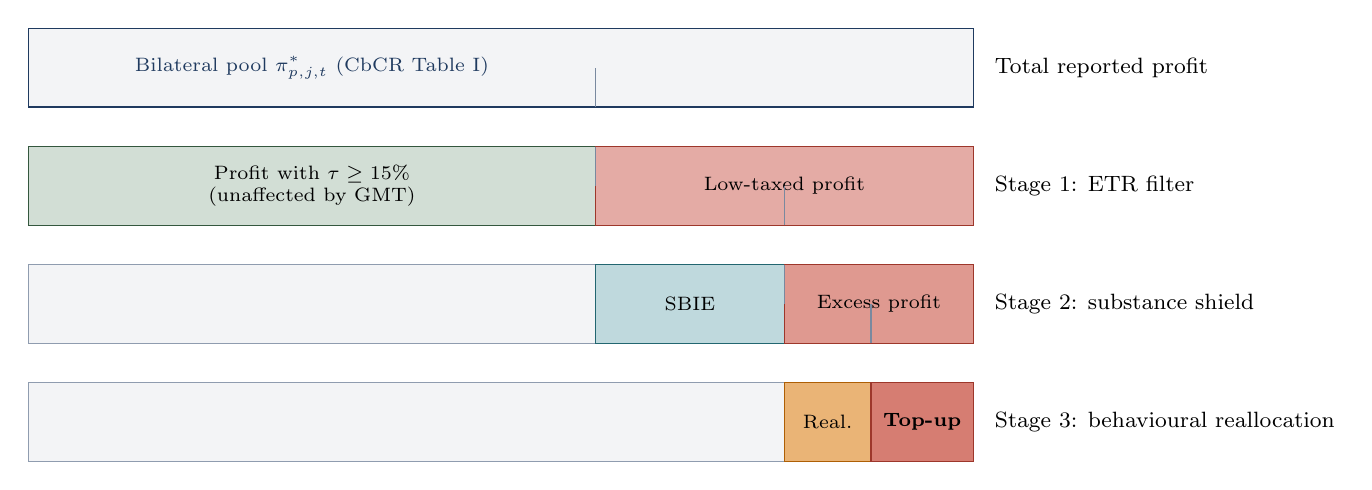
\begin{tikzpicture}[font=\small]
  % Total profit bar
  \def\tw{12}
  \def\th{1.0}

  % Layer 1: total profit
  \fill[thesisLight, draw=thesisNavy, line width=0.6pt] (0,4) rectangle (\tw, 4+\th);
  \node[font=\footnotesize, anchor=west] at (\tw+0.15, 4+\th/2) {Total reported profit};

  % Layer 2: split into above-15 (left) and below-15 (right)
  \fill[thesisGreen!25, draw=thesisGreen!70!black] (0,2.5) rectangle (7.2, 2.5+\th);
  \fill[thesisRed!45, draw=thesisRed!80!black] (7.2,2.5) rectangle (\tw, 2.5+\th);
  \node[font=\scriptsize, align=center] at (3.6, 2.5+\th/2) {Profit with $\tau \geq 15\%$\\(unaffected by GMT)};
  \node[font=\scriptsize, align=center] at (9.6, 2.5+\th/2) {Low-taxed profit};
  \node[font=\footnotesize, anchor=west] at (\tw+0.15, 2.5+\th/2) {Stage 1: ETR filter};

  % Layer 3: SBIE shield on the low-taxed portion
  \fill[thesisLight, draw=thesisNavy!50] (0,1.0) rectangle (7.2, 1.0+\th);
  \fill[thesisTeal!30, draw=thesisTeal!80!black] (7.2,1.0) rectangle (9.6, 1.0+\th);
  \fill[thesisRed!55, draw=thesisRed!80!black] (9.6,1.0) rectangle (\tw, 1.0+\th);
  \node[font=\scriptsize] at (8.4, 1.0+\th/2) {SBIE};
  \node[font=\scriptsize, align=center] at (10.8, 1.0+\th/2) {Excess profit};
  \node[font=\footnotesize, anchor=west] at (\tw+0.15, 1.0+\th/2) {Stage 2: substance shield};

  % Layer 4: behavioural response carves into the excess profit
  \fill[thesisLight, draw=thesisNavy!50] (0,-0.5) rectangle (9.6, -0.5+\th);
  \fill[thesisOrange!55, draw=thesisOrange!80!black] (9.6,-0.5) rectangle (10.7, -0.5+\th);
  \fill[thesisRed!70, draw=thesisRed!80!black] (10.7,-0.5) rectangle (\tw, -0.5+\th);
  \node[font=\scriptsize, align=center] at (10.15, -0.5+\th/2) {\rotatebox{0}{Real.}};
  \node[font=\scriptsize, align=center] at (11.35, -0.5+\th/2) {\textbf{Top-up}};
  \node[font=\footnotesize, anchor=west] at (\tw+0.15, -0.5+\th/2) {Stage 3: behavioural reallocation};

  % Connecting brackets
  \draw[thesisNavy!60, line width=0.4pt] (7.2, 4) -- (7.2, 3.5+\th);
  \draw[thesisNavy!60, line width=0.4pt] (7.2, 2.5+\th) -- (7.2, 2.0+\th);
  \draw[thesisNavy!60, line width=0.4pt] (9.6, 2.5) -- (9.6, 2.0+\th);
  \draw[thesisNavy!60, line width=0.4pt] (9.6, 1.0+\th) -- (9.6, 0.5+\th);
  \draw[thesisNavy!60, line width=0.4pt] (10.7, 1.0) -- (10.7, 0.5+\th);

  % Annotations
  \node[font=\scriptsize, thesisNavy] at (3.6, 4+\th/2) {Bilateral pool $\pi^{*}_{p,j,t}$ (CbCR Table I)};
\end{tikzpicture}
\caption[GMT design features as successive filters.]{Three design features of the GMT, applied as successive filters to the bilateral profit pool. Stage 1 isolates the low-taxed mass (red), which the jurisdiction-average and within-jurisdiction-distributional approaches measure differently. Stage 2 applies the substance-based income exclusion, shielding a fraction $\bar{\phi}_{p,j,t}$ of the low-taxed profit on the basis of payroll and tangible assets. Stage 3 removes the share that MNEs reallocate behaviourally once the effective floor rises. Only the residual (dark red) yields a top-up tax. Each stage maps to one or more factors in the variance decomposition of Section \ref{sec:decomposition}.}
\label{fig:gmt_mechanics_intro}
\end{figure}

Four findings are expected. The logarithmic specification dominates the linear and quadratic alternatives, and the panel semi-elasticity at $\tau = 0.05$ exceeds the meta-regression consensus of 0.8 \citep{heckemeyer2017} by at least a factor of three. ETR measurement accounts for the largest share of revenue variation in the factorial decomposition, consistent with the magnitude of the distributional correction documented by \citet{hugger2026}. Factor interactions exceed 10\% of total variance, indicating that one-at-a-time sensitivity analysis understates the true uncertainty range. The SbS Safe Harbour turns net GMT revenue negative for Member States that rely on the UTPR channel without a domestic QDMTT, because these countries lose collection rights on US-parented MNE groups without a backstop.


\subsection{Societal relevance}\label{sec:relevance}

The GMT is already being priced into European public budgets, and the projections rest on methodological choices whose sensitivity has been underdeveloped in academic literature. The Dutch Ministry of Finance has built \EUR466 million of projected GMT revenue into its medium-term fiscal framework \citep{36369_3}, with 86\% of revenue due to the assumed behavioural response (profit that MNEs would no longer shift to low-tax jurisdictions once the floor binds). This was adjusted downward by \EUR122 million after the January 2026 Side-by-Side package \citep{1028}. Making the link between assumptions and revenue explicit is therefore a prerequisite for fiscal planning around the reform.

Tax competition has compressed corporate tax bases across Europe \citep{cassee2019}, and low-income countries lose a disproportionate share of revenue to profit shifting \citep{cobham2018,garcia-bernardo2024}. Country-level estimates that trace projected revenue to a specific modelling choice are a direct input to ongoing implementation negotiations. The thesis provides these estimates for all 27 EU Member States, allowing finance ministries, the European Commission and the OECD to identify which assumption drives which number.

\subsection{Scientific contribution}\label{sec:contribution}

The thesis delivers four contributions to the GMT revenue literature. First, it provides the first panel estimate of profit-shifting semi-elasticities on seven years of OECD CbCR data (2016--2022) with bilateral parent--affiliate fixed effects. Earlier estimates rely on a single country \citep{dowd2017,boukal2026} or a single cross-section \citep{garcia-bernardo2024}. The panel structure absorbs time-invariant bilateral confounders (treaty networks, legal-system similarity, persistent MNE group structure) that cross-sectional designs cannot separate from the tax effect. Three functional forms (linear, quadratic, logarithmic) are estimated on the same sample and ranked by BIC, producing directly comparable semi-elasticity schedules across the ETR distribution.

Second, the thesis embeds the estimated semi-elasticity in a $2^5$ full factorial design together with four further binary modelling choices. The 32 resulting revenue scenarios are decomposed through an ANOVA identity that attributes variation exactly to five main effects and all their interactions. Existing studies vary assumptions one at a time \citep{barake2022,hugger2026} or decompose revenue by collection channel for a single country \citep{boukal2026}. The factorial design reveals whether interactions between assumptions (e.g.\ the behavioural response amplified by the distributional ETR approach) exceed the main effects, a question that one-at-a-time analysis cannot answer.

Third, the thesis constructs sector-specific effective tax floors for 27 EU Member States by combining CbCR aggregate levels with post-2021 Eurostat FATS sectoral shares. The combination exploits the complementarity of the two datasets: CbCR has tax data but no sectoral breakdown; FATS has sectoral detail but no tax data. No published study combines CbCR with FATS for sectoral GMT analysis.

Fourth, the thesis cross-validates the percentile-based distributional ETR fit from CbCR Table I against the direct subsidiary-level ETR brackets in CbCR Table IV\@. Table IV observes the profit mass below 15\% without distributional extrapolation. No study has tested whether a five-percentile piecewise-uniform fit recovers this directly observed low-taxed share, and the cross-validation quantifies the approximation error.

The remainder of this proposal is organised as follows. Section \ref{sec:litreview} reviews the profit-shifting literature, the GMT base mechanics, and theoretical models of tax competition under minimum taxation, and develops the five hypotheses. Section \ref{sec:methodology} presents the data, the revenue pipeline, the panel estimation, and the factorial decomposition. Section \ref{sec:feasibility} discusses feasibility and risks. Section \ref{sec:timeline} lists the timeline.

\newpage
\section{Literature review}\label{sec:literature}

This section reviews three strands of literature that inform the estimation framework. Section \ref{sec:beps} covers the empirical measurement of profit shifting, establishing the magnitudes that the GMT targets. Section \ref{sec:design} examines the GMT's design, revenue mechanics and the role of the substance-based income exclusion. Section \ref{sec:theory_lit} reviews theoretical models of tax competition under minimum taxation. Throughout, the review identifies what each contribution delivers and where its limitations create the gaps that this thesis addresses.

\subsection{The empirical measurement of base erosion and profit shifting}\label{sec:beps}

The Global Minimum Tax was designed around the premise that MNEs shift substantial volumes of profit to low-tax jurisdictions, eroding the tax base of countries where real economic activity occurs. Quantifying the magnitude of this shifting has been a central concern of the literature for over three decades.

\subsubsection{Methodological foundations}

The foundational approach to estimating profit shifting is surveyed by \citet{heckemeyer2017}, who identify a consensus tax semi-elasticity of reported profits of approximately 0.8. This estimate, derived from a meta-regression of 27 studies, implies that a one percentage point reduction in the tax rate differential is associated with a 0.8\% increase in reported pre-tax profits. They also conclude that transfer pricing and strategic location of intellectual property account for approximately 82\% of observed BEPS, with debt shifting responsible for the remaining 18\%.\footnote{The 82\%/18\% split is the preferred estimate from \citet{heckemeyer2017}. An alternative calculation using the debt-ratio control yields 67\%/33\%. The range across all six specifications in their Table 5 places the non-financial share at a minimum of two thirds.} The meta-regression imposes a constant semi-elasticity across the tax rate distribution, which masks the nonlinearity that subsequent work reveals at low ETRs. \citet{dharmapala2014} surveys the empirical literature on BEPS and reaches the same consensus semi-elasticity of approximately 0.8, drawing on the \emph{Hines-Rice approach} that regresses the logarithm of reported profits on the tax rate, controlling for real economic activity through labour and capital inputs. \citet{huizinga2008} extend this framework to a multilateral setting using Amadeus data, estimating a semi-elasticity of 1.3. \citet{riedel2018} provides a subsequent review that largely confirms this consensus, noting that channel-specific studies (examining debt shifting and transfer pricing separately) tend to produce the most credible estimates.

\subsubsection{Nonlinear profit shifting}

An insight for the GMT is that profit-shifting behaviour is highly nonlinear across the tax rate distribution. \citet{dowd2017} demonstrate this using US Internal Revenue Service administrative tax return data on Controlled Foreign Corporations covering 2002--2012. Their quadratic specification reveals that the semi-elasticity at a 5\% statutory tax rate is approximately 4.7, compared to only 0.7 at a 30\% rate.\footnote{These semi-elasticities are evaluated at statutory rates, not effective tax rates. Using average (effective) tax rates, \citet{dowd2017} report a semi-elasticity of 3.1 at 5\% and $-0.5$ at 30\%. The distinction matters when applying these coefficients to CbCR effective tax rates, which average 6.9 percentage points below statutory rates \citep{hugger2026}.} This implies that a one percentage point reduction in the tax rate at the very bottom of the distribution induces nearly seven times more profit shifting than the same reduction at moderate rates. The practical consequence is sizeable: in a simulation that raises six haven jurisdictions (Bermuda, the Cayman Islands, Ireland, Luxembourg, the Netherlands and Switzerland) to a 29\% statutory rate, the quadratic model predicts a \$116 billion reduction in shifted profits, roughly double the \$55--76 billion predicted by the linear model. \citet{garcia-bernardo2024} formalise this insight by developing a \emph{logarithmic} specification for the relationship between reported profits and effective tax rates. Their methodology, applied to OECD CbCR data for 2017, yields an estimate of \$850 billion in shifted profits, higher than the \$616 billion estimated by \citet{torslov2023} for 2015, partly because the log specification better captures the concentration of shifting at very low rates. Furthermore, \citet{garcia-bernardo2024} find that lower-income countries lose a larger share of total tax revenue to profit shifting than high-income countries, a finding with direct implications for the distributional assessment of the GMT.

\subsubsection{Aggregate estimates of profit shifting}

The aggregate scale of profit shifting has been estimated through two broad approaches: micro-level firm data and macro-level national accounts. The most influential macro-level study is by \citet{torslov2023}, who use Foreign Affiliates Statistics to compare the profitability of foreign-owned and locally-owned firms within each jurisdiction. Their preferred estimate is that 36\% of multinational profits (approximately \$616 billion in 2015) were shifted to tax havens, with US multinationals shifting roughly twice as much as multinationals from other parent countries relative to the size of their foreign earnings. The European Union is the biggest loser of tax revenue, with corporate tax revenue reduced by an estimated 20\% for non-haven EU countries. Tax haven affiliates display profit-to-wage ratios that are an order of magnitude higher than those of local firms in the same jurisdiction. Their methodology relies on the assumption that locally-owned and foreign-owned firms in the same jurisdiction would earn the same return on labour absent profit shifting, an assumption that breaks down in jurisdictions where foreign firms are systematically selected into higher-productivity sectors.

\citet{garcia-bernardo2024} produce a complementary estimate using OECD CbCR data, finding that MNEs shifted over \$850 billion in 2017. Their logarithmic specification captures the extreme concentration of shifted profits at very low ETRs and identifies the Cayman Islands, Luxembourg, Singapore, the Netherlands, Switzerland, Hong Kong, Bermuda, Puerto Rico and Ireland as the primary destinations. The cross-sectional design cannot control for time-invariant bilateral confounders, and the 2017 CbCR vintage is affected by the double-counting issues that \citet{blouin2023} document. \citet{garcia-bernardo2022a} test whether the 2017 US Tax Cuts and Jobs Act (TCJA) reduced profit shifting by US MNEs. They find that the share of foreign profits booked in tax havens remained stable at approximately 50\% between 2015 and 2020, despite a 3--5 percentage-point decline in the share of profits booked abroad overall. The persistence of tax-haven profit shares after a major reform that narrowed the US--haven tax differential is indirect evidence that profit shifting responds nonlinearly to tax rate changes: the TCJA narrowed the differential at moderate rates but left the incentive at very low ETRs largely intact.

\subsubsection{The double-counting critique}

A challenge to these estimates comes from \citet{blouin2023}, who demonstrate that standard data sources (US Bureau of Economic Analysis data, US IRS Form 5471, and Orbis/Bureau Van Dijk) suffer from systematic double counting and misattribution of foreign affiliate income. The equity method of accounting causes the same dollar of profit to be counted multiple times when ownership is structured through intermediate holding companies, a practice that expanded dramatically after the 1997 US ``check-the-box'' regulations. When \citet{blouin2023} replicate the revenue loss estimate of \citet{clausing2016} using the corrected measure ``Net Income Excluding Equity Income'', the estimate falls from \$77--111 billion to approximately \$11 billion, a reduction of roughly 90\%. Their reanalysis of \citet{torslov2023} suggests that the bilateral imputation of \$306 billion in shifted profits contains substantial equity income, and that removing this component reduces the total estimate by approximately half.


\subsubsection{Firm-level evidence}

\citet{johansson2017} provide large-scale firm-level evidence using the Orbis database, with 1.2 million observations across multiple countries. They find that the largest MNEs reduce their effective tax rates by 4--8.5 percentage points through a combination of profit shifting and the exploitation of tax mismatches. The estimated global corporate income tax revenue loss ranges from 4\% to 10\%. \citet{bilicka2026} exploit variation in German municipal business tax rates across over 11{,}000 municipalities during 2008--2019, finding that subsidiaries of MNEs with affiliates in tax havens respond significantly more to local tax rate increases than other firms. After a rate increase, tax revenues decline in municipalities more exposed to these aggressive MNEs, while real activities (assets and employment) remain unchanged, consistent with profit reallocation rather than real relocation. The finding supports the nonlinear profit-shifting response: firms with existing low-tax structures shift more aggressively at the margin.

The representativeness of firm-level databases is itself a methodological concern. \citet{kalemli-ozcan2015} provide critical guidance on constructing nationally representative samples from Orbis. \citet{torslov2023} show that Orbis lacks data in low-tax jurisdictions where publishing financial statements is not mandatory. For the US, Ireland, and Switzerland, no income data are available. In 2012, only 17\% of global profits appeared in Orbis, and over 80\% of subsidiaries were unknown to the database.

\subsubsection{Effects of transparency on profit shifting}

\citet{tuinsma2025} exploit the EUR 750 million revenue threshold for CbCR filing in a regression discontinuity design using Orbis data on EU-headquartered MNEs. Private CbCR raised ETRs of affected MNEs by approximately 6 percentage points relative to firms just below the threshold. The effect is concentrated in moderately aggressive firms (low pre-CbCR ETRs but no tax-haven affiliates); the most aggressive MNEs with established haven structures showed only moderate responses. The finding implies that the CbCR panel used in this thesis captures a population whose tax behaviour was itself shifting during the sample period, a consideration for the panel estimation (Section \ref{sec:estimation}).

\subsection{GMT design, revenue mechanics and implementation}\label{sec:design}

\subsubsection{Revenue estimates}

\citet{barake2022} provide the first systematic estimate of GMT revenue effects under Pillar Two. Using a combination of CbCR and FATS data, they calculate that a 15\% minimum effective tax rate would generate approximately \EUR 179 billion globally\footnote{This figure assumes that all profit within a jurisdiction faces the jurisdiction-average ETR, either fully above or fully below 15\%. As \citet{hugger2026} demonstrate, 53.2\% of globally low-taxed profit lies in jurisdictions with above-15\% average ETRs, so the true GMT base is substantially larger than Barake's estimate implies. \citet{barake2022} acknowledge this limitation but lack the within-jurisdiction ETR data needed to correct it.} and \EUR 55 billion within the EU, under an IIR-first scenario. These are first-stage estimates that assume no behavioural response by MNEs. The actual revenue depends critically on whether the top-up tax is collected by the jurisdiction of the ultimate parent entity through the IIR, or by the source country through a QDMTT.

\citet{janeba2023} develop a strategic tax competition model that produces a more nuanced picture. Their finding is that the revenue effect of the GMT depends on whether governments use distortionary or lump-sum instruments to compete for real economic activity. When instruments are distortionary, the GMT reduces profit shifting but may intensify competition among non-haven countries for real investment, potentially offsetting a portion of the revenue gains.

\subsubsection{The substance-based income exclusion}

A feature of the GMT is the SBIE, which excludes from the top-up tax calculation an amount equal to a percentage of eligible payroll costs and tangible assets located in each jurisdiction. During the transition period (2024--2033), the carve-out starts at 10\% of payroll and 8\% of tangible assets, declining to 5\% of each. \citet{devereux2023} provide the first empirical assessment of the SBIE using Amadeus data on foreign-owned EU subsidiaries, finding that the average ratio of SBIE to pre-tax profit is 57\% (52\% median), declining to 41\% (28\% median) after the ten-year transition. This implies that the average minimum tax on GloBE income is only 6.45\% in the first transition year, rising to 8.85\% at long-run rates, well below the headline 15\%. Approximately 30\% of foreign-owned EU subsidiaries in scope have SBIE exceeding pre-tax profit, facing zero top-up tax regardless of their ETR.

\citet{schjelderup2024} analyse the economic implications of the SBIE within a formal model. They reach the conclusion that the SBIE functions as a \emph{de facto} production subsidy in low-tax jurisdictions. By tying the exclusion to tangible assets and payroll, the GMT inadvertently incentivises MNEs to increase their real economic presence in low-tax locations, thereby expanding the exclusion and reducing the top-up tax. This creates a capital demand distortion that partially offsets the reduction in transfer pricing distortions that the GMT otherwise achieves. Quantitatively, the effective reduction in the rental cost of capital (0.50--0.96\%) exceeds the reduction in the effective wage rate (up to 0.88\%), implying that the SBIE \emph{favours capital-intensive industries}.

\subsubsection{Within-jurisdiction heterogeneity}

\citet{hugger2026} provide what is the most important empirical finding for understanding the actual reach of the GMT. Using confidential ETR data at the MNE-jurisdiction level, they demonstrate that 53.2\% of all low-taxed profit (below 15\% ETR) is located in jurisdictions where the \textit{average} ETR exceeds 15\%. The within-jurisdiction dispersion in ETRs is often larger than the cross-jurisdiction dispersion. This finding implies that jurisdiction-level analyses (which use average ETRs) substantially underestimate the amount of low-taxed profit and, correspondingly, the potential revenue from the GMT.

\subsubsection{Tax incentives under Pillar Two}

\citet{ferreiraliotti2022} examine how existing tax incentives interact with the GMT. The impact varies dramatically by type: accelerated depreciation provisions have a low impact because they primarily affect timing rather than the level of taxation, whereas tax holidays and IP box regimes have a significant impact because they reduce the ETR below 15\%. The QDMTT serves as a safety valve that allows countries to retain the top-up tax domestically, but this also means that the incentive offered to the MNE is effectively nullified.

\subsection{Theoretical models of the GMT and tax competition}\label{sec:theory_lit}

\subsubsection{Welfare effects}

\citet{johannesen2022} develops the first formal model specifically designed to analyse the welfare effects of the GMT. The model features a large country (non-haven) and a small country (haven) that compete for mobile profits. The central result is that the welfare effect for the non-haven country is \textit{ambiguous}: it is positive when the profit-shifting response to taxation is strong and when the government places a low weight on the consumption of firm owners relative to public goods. The consensus semi-elasticity of 0.8 falls below even the lowest of the required thresholds (which range from roughly 1.8 to 4.2 depending on the marginal social value of public funds and the initial haven tax rate; Table 1 in \citealp{johannesen2022}), but the quadratic specification of \citet{dowd2017} exceeds them all at ETRs below roughly 9\%, precisely the range in which the GMT base is concentrated.

\citet{hebous2023} contribute to this debate by identifying conditions under which a minimum corporate tax can be Pareto-improving: all countries, including havens, can be made better off if the minimum tax is combined with appropriate transfers. \citet{vantriet2025} provide the first quantitative welfare assessment, simulating the GMT in the CORTAX macroeconomic model for the EU-27, the US, the UK, Japan, and a generic tax haven. Under their preferred closure (additional CIT revenue recycled as lower CIT rates), the GMT produces modestly positive global welfare, and the optimal minimum rate is 16\%. The simulation satisfies the Hicks--Kaldor compensation test, indicating a potential Pareto improvement. Their model does not incorporate the nonlinear semi-elasticities that \citet{dowd2017} document, however, and uses a representative-firm framework that cannot capture within-jurisdiction ETR heterogeneity.

\subsubsection{Tax competition under the GMT}

\citet{janeba2023} model the strategic interaction between countries after GMT implementation. Their model distinguishes between profit-shifting channels (which the GMT constrains) and real-activity channels (which it does not). The GMT eliminates the incentive for havens to set rates below 15\%, but it simultaneously increases the incentive for non-havens to compete for real economic activity through subsidies, infrastructure investment, and regulatory competition.

\citet{schjelderup2024} extend this analysis by incorporating the SBIE into a two-country model. They show that the SBIE transforms the GMT from a pure anti-avoidance instrument into a hybrid policy that simultaneously discourages profit shifting (through the minimum tax) and encourages real investment in low-tax jurisdictions (through the substance exclusion). The net effect on the allocation of capital is theoretically ambiguous and depends on the elasticity of transfer pricing relative to the elasticity of real capital demand.

\subsubsection{The enforcement dilemma}

\citet{jean2026} introduce a fundamentally different concern: the GMT may undermine the international cooperation that is necessary for effective tax enforcement. In their game-theory model, two countries (high-tax and low-tax) choose both tax rates and enforcement effort. The GMT reduces the incentive for the low-tax country to cooperate on enforcement, because the top-up tax is collected by the high-tax country. When the minimum rate exceeds a critical threshold, the low-tax country prefers to withdraw from enforcement cooperation entirely. This creates a paradox: the GMT reduces profit shifting in the short run but may increase it in the long run by destroying the cooperative enforcement equilibrium.
\newpage

\section{Data and descriptive statistics}\label{data}

The estimation framework draws on two primary data sources and several supplementary datasets. The OECD Country-by-Country Reporting (CbCR) statistics provide the bilateral profit, tax, payroll, asset, and ETR distribution data that form the backbone of the revenue pipeline. Eurostat inward Foreign Affiliates Statistics (FATS) supply the sectoral decomposition of economic activity within EU Member States that CbCR lacks. CbCR has no sectoral breakdown, and FATS has no tax data. 

\subsection{OECD CbCR data}\label{CbCR}

BEPS Action 13 requires large MNE groups with consolidated revenue exceeding \EUR750 million to file Country-by-Country Reports detailing their economic activity and tax payments in each jurisdiction where they operate.\footnote{The \EUR750 million threshold was chosen by the OECD to balance coverage against compliance burden. Since Pillar Two applies to the same threshold population, the CbCR scope aligns with the GMT's statutory scope. The threshold excludes smaller MNEs that may face systematically different ETRs. This is not a limitation for revenue estimation but matters for welfare analysis.} The OECD aggregates and anonymises these filings into jurisdiction-level statistics published in the Corporate Tax Statistics (CTS) database.\footnote{The data can be found via the OECD Data Explorer, Taxation, Corporate Tax. Under this view, as of April 2026, 19 datasets appear. The six CbCR tables can be filtered out of these. This \href{https://data-explorer.oecd.org/?fs\%5B0\%5D=Topic\%2C1\%7CTaxation\%23TAX\%23\%7CCorporate\%20tax\%23TAX_CPT\%23&pg=0&fc=Topic&bp=true&snb=19}{link} also references the data.}

The CbCR dataset is suited for GMT revenue estimation, since it captures tax-planning behaviour across virtually all jurisdictions, including low-tax locations that are absent from firm-level databases such as Orbis or Compustat.\footnote{Firm-level databases suffer from selection bias in low-tax jurisdictions because MNEs operating through shell entities in these locations often have no obligation to file public financial statements \citep{torslov2023}. CbCR data are filed with the parent jurisdiction's tax authority and reported to the OECD regardless of the affiliate jurisdiction's disclosure regime \citep{oecd2025a}.} Second, the bilateral parent--affiliate structure mirrors the GMT's own architecture: the top-up tax is computed jurisdiction by jurisdiction for each MNE group, allocated through the Income Inclusion Rule to the parent and through the UTPR to affiliate jurisdictions.

The CbCR database is organised into six tables, each constructed from the same underlying filings but aggregated along different dimensions. Table \ref{tab:crosssummary} summarises their structure. Coverage expanded substantially over the period as more jurisdictions enacted BEPS Action 13 legislation: 26 parent jurisdictions reported in 2016, rising to 54 by 2022, representing approximately 98\% of all CbCR filings globally \citep{oecd2025a}.\footnote{Table \ref{tab:yearcoverage} in Appendix \ref{app:CbCR} documents the year-by-year expansion of reporting coverage in Table I.}

\begin{table}[H]
\centering
\caption{Cross-table summary of OECD CbCR Tables I--VI}
\label{tab:crosssummary}
\footnotesize
\begin{tabular}{@{}lrrrrrrr@{}}
\toprule
 & \textbf{Table I} & \textbf{Table II} & \textbf{Table III} & \textbf{Table IV} & \textbf{Table V} & \textbf{Table VI} \\
 & Agg.\ Totals & IQ Means & ETR (MNE) & ETR (Sub.) & Size Dist.\ & Size Agg.\ \\
\midrule
Rows (total) & 1,124,211 & 437,129 & 699,246 & 101,399 & 4,195 & 105,753 \\
Positive obs (\%) & 71.5 & 84.6 & 68.3 & 77.3 & 98.4 & 72.1 \\
Zero obs (\%) & 21.7 & 7.6 & 24.9 & 12.1 & 0.4 & 22.9 \\
NaN / missing (\%) & 3.0 & 1.9 & 3.6 & 6.5 & 1.1 & 2.4 \\
\addlinespace
Fiscal years covered & 2016--2022 & 2017--2022 & 2017--2022 & 2016--2022 & 2016--2022 & 2022 only \\
Parent jurisdictions & 58 & 46 & 46 & 49 & 40 & 39 \\
Affiliate jurisdictions & 240 & 238 & 238 & 154 & -- & 215 \\
Number of MEASURE codes & 28 & 14 & 27 & 27 & 3 & 26 \\
\addlinespace
Aggregation type & \code{TOTAL} & \code{TOTAL} & \code{TRMNE} & \code{TRSUB} & \code{TRMNE} & \code{MNESIZE} \\
ETR brackets & No & No & Yes (12) & Yes (11) & No & No \\
Profit panels & A-I, A-II & A-I, A-II & -- & -- & -- & -- \\
Statistical operations & Pct., Agg & IQmean & Agg & Agg & Pctiles & Agg \\
MNE size classes & No & No & No & No & No & Yes (6) \\
\bottomrule
\end{tabular}
\end{table}

Tables I and IV carry the bulk of the information the revenue pipeline exploits, and they complement each other: Table I supplies the aggregate financial levels together with summary percentiles of the within-jurisdiction ETR distribution, while Table IV partitions the same financial variables into 11 ETR brackets at the subsidiary level. Neither table dominates the other. Table I has broader coverage (58 vs.\ 49 parents and 240 vs.\ 154 affiliate jurisdictions) and is the only source of percentile moments ($P5, P25, P50, P75, P95$); Table IV has narrower coverage but observes directly the profit mass inside the GMT-critical $[0, 15\%)$ bracket. Stage 1 of the methodology therefore uses Table I for distributional fitting and Table IV for direct observation, combining them in the hybrid measurement of Section \ref{sec:crossval}. The other four tables supply supporting information (Section \ref{sec:other_tables}).

\subsubsection{Table I: aggregate totals and ETR percentiles}\label{sec:t1_main}

Table I is the starting point for the revenue pipeline. It reports jurisdiction-level financial aggregates for each bilateral parent--affiliate pair, creating a dataset analogous to a trade matrix: each cell represents the total economic activity of all MNEs headquartered in parent jurisdiction $p$ that have constituent entities in affiliate jurisdiction $j$. The financial measures include profit before income tax (\code{PROFIT}), adjusted profit (\code{PROFIT\_ADJ}, available for 2021--2022), income tax accrued (\code{TAX\_ACCRUED}), total payroll (\code{EARNINGS}), tangible assets (\code{ASSETS}), and employee counts (\code{EMPLOYEES}), among 28 measure codes in total.\footnote{Appendix \ref{app:CbCR}, Table \ref{tab:measures}, provides the full list of measure codes. Monetary values are denominated in USD.}

Table I is also the only CbCR table that reports moments of the within-jurisdiction ETR distribution, through five bilateral percentiles ($P5, P25, P50, P75, P95$) on the \code{ETR} measure. These percentiles are the empirical input to the distributional Stage 1 approach developed in Section \ref{sec:distributional}: they are the finest shape information publicly available, and any distributional fit to CbCR data must be anchored on them. Two profit panels are reported: Panel A-I restricts to profit-making entities (positive profit before tax) and is used as the denominator for all ETR calculations; Panel A-II adds loss-makers and is used only where total activity coverage is required.

Table I further reports business-activity counts: the number of constituent entities in each bilateral cell classified by primary business activity (holding, IP management, manufacturing, R\&D, finance, and others). The holding-company share (\code{ACT\_HOLDING}/\code{ENTITIES\_COUNT}) is central to the profit-base correction developed in Section \ref{sec:doublecounting}, and the activity composition of the low-tax bracket is an input to the SBIE allocation (Section \ref{sec:sbie_decomp}).

Table I covers 58 parent jurisdictions and 240 affiliate jurisdictions in its most complete vintage (2022). The affiliate dimension includes individual country codes, regional aggregates, and a ``world excluding domestic'' aggregate (\code{WXD}) that captures all foreign affiliate activity.\footnote{Appendix \ref{app:CbCR} documents the full set of aggregate codes. The bilateral structure means that the same affiliate jurisdiction appears in multiple rows, once for each parent jurisdiction that reports MNE activity there.}

\subsubsection{Table IV: subsidiary-level ETR brackets}\label{sec:t4_main}

Table IV performs the complementary task: it partitions all financial variables by 11 ETR brackets at the \emph{subsidiary} level, so the ETR assigned to each observation reflects the individual constituent entity's own jurisdictional effective tax rate, not the MNE group's global average.\footnote{This contrasts with Table III, which assigns ETR brackets at the MNE-group level. \citet{hugger2026} demonstrate that 53.2\% of all low-taxed profit is located in jurisdictions where the \emph{jurisdiction-average} ETR exceeds 15\%, so any aggregation to the jurisdiction mean obscures more than half of the GMT base. Table III's MNE-group aggregation operates on a different axis but raises the same concern; Table IV, which brackets at the subsidiary level, resolves both.} The \code{RATE\_0-15} bracket directly identifies all profit, assets, payroll, and tax reported by entities facing an ETR below 15\%: the GMT top-up base without any distributional extrapolation.

Because Table IV observes the quantity that Stage 1's distributional fit must estimate, it plays two roles in the methodology: (i) as the preferred data source inside the hybrid measurement \eqref{eq:hybrid} wherever it is observed, and (ii) as the independent benchmark against which the Table I distributional fit is cross-validated (Section \ref{sec:crossval}). The second role is what makes the approximation error of the five-percentile fit quantifiable rather than assumed.

Table IV covers 49 parent jurisdictions and 154 affiliate jurisdictions. The reduced affiliate coverage relative to Table I (154 vs.\ 240) reflects OECD confidentiality thresholds: jurisdictions with too few MNE affiliates are suppressed to prevent identification of individual MNE groups. The restriction is not binding for the EU analysis: all 27 EU Member States appear in Table IV as affiliate jurisdictions, and Table IV is therefore the primary Stage 1 source for the EU sample. The distributional fit on Table I provides the extension to non-EU affiliates where Table IV is unavailable.

\subsubsection{Tables II, III, V, and VI}\label{sec:other_tables}

The remaining four tables serve supporting roles. Table II reports interquartile means (IQM) of financial variables, the arithmetic mean computed after excluding the bottom and top quartiles of MNE groups within each bilateral pair. This robust central tendency estimator is less sensitive to the extremely large MNE groups that dominate simple averages; it serves as a cross-check on the aggregate totals in Table I for the SBIE computation. Table III disaggregates observations by ETR bracket at the MNE-group level and is therefore less suitable for direct GMT revenue computation than Table IV, but it provides business-activity counts within each ETR range that are informative about the composition of low-taxed activity. Table V reports the size distribution of MNE groups within each parent jurisdiction through seven percentile points (P5 through P95), enabling characterisation of MNE groups near the \EUR750 million threshold. Table VI, the most recently added dimension, breaks down all financial and activity variables by five MNE group revenue size classes for fiscal year 2022 only.

\subsubsection{Temporal scope and lag}\label{sec:temporal}

The most recent CbCR release covers fiscal year 2022, published in November 2025 \citep{oecd2025a}. The lag of approximately three years between fiscal year and public availability means that implementation data is not yet available. The estimation is therefore necessarily backward-looking: it applies the GMT rules to pre-implementation data (2016--2022) and projects revenue prospectively. The 2016--2022 panel nevertheless provides seven years of pre-reform variation in ETRs, sufficient for the within-pair identification strategy developed in Section \ref{sec:estimation}.

\subsubsection{Correcting the profit base}\label{sec:doublecounting}

Public CbCR profit data suffer from systematic double counting through intra-group dividends and ownership chains. When a German parent owns a Dutch holding company that in turn owns an Irish operating subsidiary, the Irish subsidiary's profits may appear in both the German CbCR filing (through the ultimate parent) and in the Dutch profits (as an intermediate holding). \citet{garcia-bernardo2022a} show that aggregate CbCR profits are overstated by 48\% in 2017, 72\% in 2018, and 47\% in 2019, with domestic American profits responsible for the bulk of the discrepancy. \citet{barake2022} estimate global GMT revenue using corrected CbCR data combined with Eurostat FATS, explicitly noting that uncorrected profit bases inflate revenue figures through profits in conduit jurisdictions.\footnote{\citet{barake2022} does not combine CbCR data with FATS themselves, they use the corrected estimates by the Working paper of \citet{torslov2023}.}

The OECD introduced the \code{PROFIT\_ADJ} measure (profit adjusted for intra-group dividends and equity income) but broad coverage first appears in 2021.\footnote{\citet{boukal2026} report that the OECD's November 2019 guidance update requires exclusion of intra-company dividends from 2020 fiscal-year data onwards, which explains why \code{PROFIT\_ADJ} coverage first appears in 2021. Compliance across reporting jurisdictions remains uneven.} The 2016--2020 panel therefore requires a backcasting procedure. \citet{hugger2026} correct UPE-level profits using information from tax authorities or domestic--foreign affiliate ETR comparisons, reaching a median correction of 32.4\% applied to roughly two thirds of UPE profit values, with the percentage reduction capped at 55.5\%. The procedure still produces a uniform downward adjustment within each jurisdiction and does not model the cross-jurisdictional variation in double-counting severity that the holding-company structure would predict. \citet{blouin2023} demonstrate that double counting through the equity method is concentrated in jurisdictions where MNEs structure ownership through intermediate holding companies, and that removing equity income from conduit jurisdictions reduces measured profit shifting by an order of magnitude. \citet{garcia-bernardo2022a} confirm this pattern in the CbCR context: domestic holding chains are responsible for the bulk of the aggregate overstatement. The OECD itself identifies a concentration of holding companies as a risk factor associated with tax planning structures \citep{oecd2025a}. Double counting is therefore not uniform across jurisdictions but varies systematically with holding-company prevalence.

The corrected profit base uses observed \code{PROFIT\_ADJ} where available and a predicted correction ratio ($\hat{\gamma}_{j,t} \cdot \code{PROFIT}_{p,j,t}$) otherwise. The prediction exploits the cross-jurisdictional variation in holding-company intensity. For each affiliate jurisdiction $j$, the observed correction ratio $\gamma_j = \pi_j^{\text{ADJ},2022} / \pi_j^{2022}$ in the 2021--2022 sample is regressed on holding-company intensity:
\begin{equation}\label{eq:correction_model}
\gamma_j = \alpha + \beta \cdot \frac{\text{ACT\_HOLDING}_j}{\text{ENTITIES\_COUNT}_j} + \varepsilon_j
\end{equation}
where $\text{ACT\_HOLDING}_j / \text{ENTITIES\_COUNT}_j$ is the share of entities classified as holding companies in CbCR Table I. A lower $\gamma_j$ indicates a larger downward adjustment after removing intra-group dividends. The hypothesis, motivated by \citet{blouin2023}, is that $\beta < 0$: jurisdictions with a higher share of holding companies exhibit more double counting and therefore require a larger correction. Fitted values extend the correction to the 2016--2020 panel: $\hat{\pi}_{j,t}^{*} = \hat{\gamma}_{j,t} \cdot \pi_{j,t}, \quad t \in \{2016, \ldots, 2020\}$. 

The holding-company share varies over time as MNE structures evolve; $\hat{\gamma}_{j,t}$ varies accordingly.\footnote{This approach assumes structural stability in the relationship between holding-company intensity and double counting over 2016--2022. The assumption is tested by estimating the model separately on 2021 and 2022 data and comparing the coefficients.} The profit-base correction enters the factorial design in three specifications: (i) no correction ($\pi^* = \pi$), providing an upper bound on the profit base; (ii) baseline, using the predicted ratio $\hat{\gamma}_{j,t}$ from equation \eqref{eq:correction_model}; and (iii) aggressive, setting $\gamma$ to the 25th percentile of the 2022 distribution, allowing larger reductions for jurisdictions with high holding and IP intensity.

\workingnote{After estimation: report $\hat{\beta}$, its standard error, and the cross-jurisdictional distribution of $\hat{\gamma}$. Discuss whether the correction ratio is stable between the 2021 and 2022 donor years.}

\subsection{Eurostat inward Foreign Affiliates Statistics}\label{sec:fats_main}

CbCR reports no sectoral breakdown. The substance-based income exclusion depends on payroll and tangible assets, both of which vary dramatically across sectors: manufacturing has high payroll and capital intensity relative to profits, while holding and IP licensing have near-zero substance. Estimating sector-specific SBIE-to-profit ratios and effective tax floors (Section \ref{sec:sbie_decomp}) requires a sectoral decomposition of economic activity that CbCR cannot provide. This is done with Eurostat inward FATS. 

The dataset covers all foreign-controlled enterprises operating inside European reporting economies, recording employment, turnover, personnel costs, and investment by NACE sector and by the controlling country of the foreign parent.\footnote{``Foreign-controlled'' is defined by majority ownership (more than 50\% of voting rights) by an entity resident outside the reporting country. The definition is broader than the CbCR in-scope population: FATS includes all foreign-controlled firms regardless of size, whereas CbCR is restricted to MNE groups with consolidated revenue above \EUR750 million. Using FATS sectoral shares on CbCR aggregate levels therefore produces conservative estimates, since the sectoral composition of all foreign-controlled firms may differ from that of the largest MNE groups alone.} In the sectoral SBIE formula (equation \ref{eq:sbie_sectoral}) FATS personnel costs provide the payroll share and FATS investment data provide the basis for imputing the tangible asset share.\footnote{FATS does not report tangible assets directly. The tangible asset share is imputed from the capital intensity (investment-to-turnover ratio) of each NACE sector. This imputation is the weakest link in the sectoral decomposition. Section \ref{sec:sbie_decomp} discusses the procedure.}

A structural break in 2021 complicates the time series. The pre-2021 series uses a single broad activity aggregate and 23 indicators, while the post-2021 series uses 48 NACE-based activity categories and 19 codes. The two halves are not directly comparable. The sectoral estimation therefore uses the post-2021 \code{fats\_activ} data only. Pre-2021 FATS serve as descriptive background. \workingnote{After data cleaning: report how many EU Member States $\times$ NACE sectors $\times$ years have complete FATS coverage in the post-2021 series. Identify any Member States with substantial missing data and describe how missing cells are handled (drop, impute, or aggregate to broader NACE categories).}

The CbCR $\times$ FATS combination restricts the sectoral analysis to the EU-27.\footnote{Three grounds justify this scope. First, all 27 EU Member States appear in both CbCR Table I and Table IV as affiliate jurisdictions. Second, FATS is an EU-specific dataset with no equivalent coverage for non-EU jurisdictions. Third, the EU implemented Pillar Two uniformly through the Minimum Tax Directive (Council Directive (EU) 2022/2523), so the institutional setting is homogeneous across the sample.} The global revenue pipeline (equation \ref{eq:pipeline}) is estimated for all jurisdictions in the CbCR data. The sectoral decomposition of effective tax floors and SBIE ratios is restricted to the EU-27.

\subsection{Supplementary data sources}\label{sec:supplementary}

The panel estimation (Section \ref{sec:estimation}) and the revenue allocation stage (Section \ref{sec:sbs}) require several additional datasets. Appendix \ref{sec:add_data} documents each source in detail; this subsection summarises their role in the estimation framework.

Statutory corporate income tax rates from the OECD Tax Database (144 jurisdictions, 2000--2025) serve two purposes: as a benchmark against which CbCR effective tax rates are compared, and as an instrument in robustness checks where the endogeneity of effective rates is a concern.\footnote{Appendix \ref{sec:cit} documents the variable codes and coverage.} The combined (central plus sub-central) rate is the relevant measure for jurisdictions with federated tax systems.

Wage data are collected from three sources to maximise country coverage. OECD average annual wages (41 countries, 1990--2024) provide the primary cross-country comparator in PPP-adjusted USD. The OECD hourly earnings index (41 countries, 1955--2026) provides a longer time series for trend analysis. ILO hourly and monthly earnings (105--140 countries, 1990--2025) extend coverage to non-OECD economies.\footnote{Appendix \ref{sec:wages_appendix} documents the three wage files, their indicators, and the hierarchy of preference (OECD first, ILO for non-OECD).} Wage data enter the estimation framework in two ways: as a control variable in the profit-shifting regressions (proxying for labour market conditions in the affiliate jurisdiction) and as the input for imputing missing CbCR payroll values. Where the \code{EARNINGS} variable is missing in CbCR, payroll is imputed as $N_{p,j,t} \times \bar{w}_{j,t}$, the product of the CbCR employee count and the jurisdiction-average annual wage (Section \ref{sec:payroll_imputation}).

World Bank macroeconomic controls (GDP per capita (current USD, 217 countries, 2015--2024) and population (217 countries, 2015--2024)) enter the Hines--Rice regression as affiliate-jurisdiction controls.\footnote{Appendix \ref{sec:worldbank} documents these variables.} Log GDP per capita proxies for the level of economic development and market size. Log population controls for country scale.

OECD BEPS implementation indicators document the adoption of anti-avoidance measures across jurisdictions: CbCR filing requirements (Action 13, 119 countries), CFC rules (146 countries), interest limitation rules (Action 4, 146 countries), hybrid mismatch rules (Action 2, 145 countries), IP regimes (Action 5, 64 countries), and mandatory disclosure rules (Action 12, 145 countries).\footnote{Appendix \ref{sec:beps_appendix} documents these indicators.} These indicators enter the factorial design as controls for the institutional environment: jurisdictions with more comprehensive BEPS implementation may exhibit different profit-shifting patterns.

Pillar Two implementation status is tracked through the PwC global Pillar Two tracker, which records the legislative status (enacted, consultation, or announced) of the IIR, UTPR, and QDMTT for each jurisdiction, together with effective start dates.\footnote{Appendix \ref{sec:pillar2} documents this source, which is cross-referenced against the OECD Central Record of Qualified Domestic Minimum Taxes.} The QDMTT indicator ($\mathbb{1}_j^{\text{Q}}$) and the SbS regime indicator ($\mathbb{1}_p^{\text{SbS}}$) used in the revenue allocation stage (Section \ref{sec:sbs}) are constructed from this tracker.

\subsection{Notation}\label{sec:notation}

Subscript $p$ denotes the parent jurisdiction (ultimate parent entity, UPE), $j$ denotes the affiliate jurisdiction, and $t$ denotes the fiscal year ($t \in \{2016, \ldots, 2022\}$). The $p,j$ convention follows \citet{barake2022}; $j$ is reserved exclusively for the affiliate jurisdiction throughout. All monetary values are in USD unless stated otherwise, consistent with CbCR reporting conventions.\footnote{CbCR data are reported in USD. No PPP adjustment is applied to the revenue calculations, since the GMT operates on nominal profit and tax liabilities denominated in the MNE group's reporting currency. PPP-adjusted wage data from the OECD and ILO are used only for imputing missing payroll values (Section \ref{sec:payroll_imputation}).} Table \ref{tab:notation} summarises the symbols used throughout.

\begin{table}[H]
\centering
\caption{Variable notation}
\label{tab:notation}
\small
\begin{tabular}{@{}ll@{}}
\toprule
Symbol & Definition \\
\midrule
$\pi_{p,j,t}$ & Reported profit before income tax (CbCR \code{PROFIT}) \\
$\pi_{p,j,t}^{*}$ & Corrected profit base (Section \ref{sec:doublecounting}) \\
$\theta_{p,j,t}$ & Income tax accrued (CbCR \code{TAX\_ACCRUED}) \\
$A_{p,j,t}$ & Tangible assets excl.\ cash and equivalents (CbCR \code{ASSETS}) \\
$W_{p,j,t}$ & Total payroll / compensation of employees (CbCR \code{EARNINGS}) \\
$N_{p,j,t}$ & Number of employees, FTE (CbCR \code{EMPLOYEES}) \\
$\bar{w}_{j,t}$ & Average annual wage in jurisdiction $j$ (OECD/ILO) \\
$\tau_{p,j,t}$ & Effective tax rate (ETR) $= \theta_{p,j,t} / \pi_{p,j,t}$ \\
$T$ & Global minimum tax rate $= 0.15$ \\
$\tau_{p,j,t}^{(k)}$ & $k$-th percentile of the ETR distribution (from Table I) \\
$s_{j,t}^{<T}$ & Share of profit with ETR below $T$ in jurisdiction $j$ \\
$\ell_{p,j,t}$ & Low-taxed profit volume $= s_{j,t}^{<T} \cdot \pi_{p,j,t}^{*}$ (Section \ref{sec:etr_measurement}) \\
$\bar{\delta}_{j,t}^{\text{top}}$ & Average top-up rate on the low-taxed portion (Section \ref{sec:etr_measurement}) \\
$\sigma_W(t), \sigma_A(t)$ & SBIE payroll and tangible assets carve-out rates (Section \ref{sec:SBIE}) \\
$\phi_{p,j,t}$ & SBIE-to-profit ratio $= \text{SBIE}_{p,j,t} / \pi_{p,j,t}^{*}$ (Section \ref{sec:SBIE}) \\
$\text{SC}_{p,j,t}^{\text{M1}}$ & Substance Cap, Method 1 (Section \ref{sec:sbti}) \\
$\text{SC}_{p,j,t}^{\text{M2}}$ & Substance Cap, Method 2 (Section \ref{sec:sbti}) \\
$\kappa_{j,s,t}$ & Sectoral SBTI-capacity proxy (Section \ref{sec:sbti_amplification}) \\
$\beta_{j,t}$ & Fraction of low-taxed profit reallocated under behavioural response \\
$\mathbb{1}_j^{\text{Q}}$ & Indicator: $=1$ if jurisdiction $j$ has implemented a QDMTT \\
$\mathbb{1}_p^{\text{SbS}}$ & Indicator: $=1$ if parent $p$ has a Qualified SbS Regime (currently US only) \\
$a_{s,p,j,t}^{(r)}$ & Allocation weight under policy regime $r$ (Section \ref{sec:sbs}) \\
$\mathbf{x}$ & Factorial configuration vector $(x_1, \ldots, x_5) \in \{0,1\}^5$ (Section \ref{sec:factorial}) \\
$\eta_i^2$ & Share of explained variance attributable to factor $i$ (Section \ref{sec:anova}) \\
$\Lambda_{j,t}$ & Ratio of scenario spread to estimation uncertainty (Section \ref{sec:two_uncertainties}) \\
\bottomrule
\end{tabular}
\end{table}

\newpage 

\section{Methodology}\label{sec:methodology}

Estimating the revenue of the GMT is based on three questions about the bilateral profit base: how much profit sits below the 15\% effective tax floor, how much of that profit survives the substance-based income exclusion, and how much survives behavioural reallocation once the floor binds. The methodology mirrors this structure. Stage 1 applies an ETR filter; Stage 2 applies the SBIE; Stage 3 applies a behavioural adjustment. Their product, allocated across QDMTT, IIR, and UTPR collection channels under the January 2026 Side-by-Side Safe Harbour, gives the estimated top-up tax for each EU Member State.

The behavioural parameter in Stage 3 (the tax semi-elasticity of reported profits) is not taken from the literature but estimated directly from the 2016--2022 CbCR panel using the Hines--Rice framework with bilateral fixed effects. The functional form of the semi-elasticity is itself uncertain; linear, quadratic, and logarithmic specifications are compared and the preferred form enters the revenue pipeline. The remaining stages each carry a contested methodological choice: how to measure the ETR, and which SBIE specification to apply. All five binary decisions are embedded in a $2^5$ full factorial design. The 32 resulting scenarios span the plausible revenue range; an ANOVA decomposition attributes variation to main effects and interactions, separating what is driven by unresolvable modelling choices from what is driven by estimation error.

The sections follow this sequence. Sections \ref{sec:etr_measurement} and \ref{sec:SBIE} develop the ETR measurement approaches and SBIE specifications respectively. Section \ref{sec:behavioural} develops the Stage 3 model; Section \ref{sec:estimation} estimates the semi-elasticity and selects the preferred functional form. Section \ref{sec:sbs} introduces the January 2026 allocation rules. Section \ref{sec:pipeline} assembles the three stages into a single multiplicative equation. Section \ref{sec:decomposition} runs the factorial experiment and ANOVA. Section \ref{sec:hypotheses} derives five testable hypotheses.

Figure \ref{fig:pipeline_schematic} summarises the architecture.\footnote{The revenue pipeline decomposition is original to this thesis. The individual components draw on \citet{hugger2026} (Stage 1), \citet{schjelderup2024} and \citet{devereux2023} (Stage 2), and the panel-estimated semi-elasticities (Section \ref{sec:estimation}) for Stage 3. No prior study combines these into a single multiplicative framework that makes the sources of revenue uncertainty simultaneously visible and exactly decomposable.}

\begin{figure}[H]
\centering
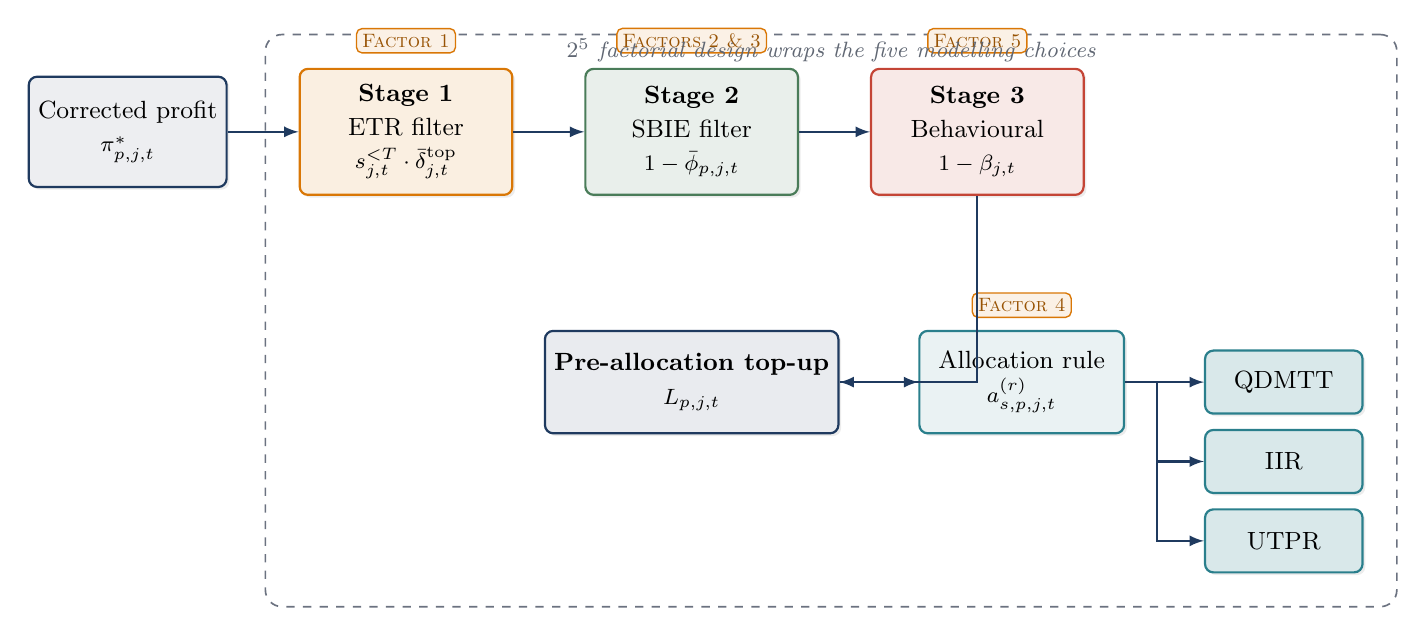
\begin{tikzpicture}[font=\small, node distance=0.85cm]
  % Input
  \node[thesis stage, fill=thesisMid!40, minimum width=2.4cm, minimum height=1.4cm] (input)
    {Corrected profit\\[1pt]\footnotesize $\pi^{*}_{p,j,t}$};

  % Stage 1
  \node[thesis stage, right=0.9cm of input, fill=thesisOrange!12, draw=thesisOrange,
        minimum width=2.7cm, minimum height=1.6cm] (s1)
    {\textbf{Stage 1}\\[1pt]ETR filter\\[1pt]\footnotesize $s^{<T}_{j,t}\cdot\bar{\delta}^{\text{top}}_{j,t}$};

  % Stage 2
  \node[thesis stage, right=0.9cm of s1, fill=thesisGreen!12, draw=thesisGreen,
        minimum width=2.7cm, minimum height=1.6cm] (s2)
    {\textbf{Stage 2}\\[1pt]SBIE filter\\[1pt]\footnotesize $1-\bar{\phi}_{p,j,t}$};

  % Stage 3
  \node[thesis stage, right=0.9cm of s2, fill=thesisRed!12, draw=thesisRed,
        minimum width=2.7cm, minimum height=1.6cm] (s3)
    {\textbf{Stage 3}\\[1pt]Behavioural\\[1pt]\footnotesize $1-\beta_{j,t}$};

  % Factor tags above each stage
  \node[thesis factor, above=0.18cm of s1] {\textsc{Factor 1}};
  \node[thesis factor, above=0.18cm of s2] {\textsc{Factors 2 \& 3}};
  \node[thesis factor, above=0.18cm of s3] {\textsc{Factor 5}};

  % Pre-allocation liability
  \node[thesis stage, below=1.7cm of s2, fill=thesisNavy!10, draw=thesisNavy,
        minimum width=3.6cm, minimum height=1.3cm] (L)
    {\textbf{Pre-allocation top-up}\\[1pt]\footnotesize $L_{p,j,t}$};

  % Allocation node
  \node[thesis alloc, right=1.0cm of L, minimum width=2.6cm, minimum height=1.3cm] (alloc)
    {Allocation rule\\[1pt]\footnotesize $a^{(r)}_{s,p,j,t}$};
  \node[thesis factor, above=0.15cm of alloc] {\textsc{Factor 4}};

  % Three channels
  \node[thesis stage, right=1.0cm of alloc, fill=thesisTeal!18, draw=thesisTeal,
        minimum width=2.0cm, minimum height=0.8cm] (qdmtt) {QDMTT};
  \node[thesis stage, below=0.18cm of qdmtt, fill=thesisTeal!18, draw=thesisTeal,
        minimum width=2.0cm, minimum height=0.8cm] (iir) {IIR};
  \node[thesis stage, below=0.18cm of iir, fill=thesisTeal!18, draw=thesisTeal,
        minimum width=2.0cm, minimum height=0.8cm] (utpr) {UTPR};

  % Forward arrows
  \draw[thesis arrow] (input) -- (s1);
  \draw[thesis arrow] (s1) -- (s2);
  \draw[thesis arrow] (s2) -- (s3);

  % Down arrow from s3 → L (elbow)
  \draw[thesis arrow] (s3.south) |- ($(L.east)+(0.6,0)$) -- (L.east);
  % Allocation
  \draw[thesis arrow] (L) -- (alloc);
  \draw[thesis arrow] (alloc.east) -- ++(0.4,0) |- (qdmtt.west);
  \draw[thesis arrow] (alloc.east) -- ++(0.4,0) |- (iir.west);
  \draw[thesis arrow] (alloc.east) -- ++(0.4,0) |- (utpr.west);

  % Factorial wrapper
  \begin{scope}[on background layer]
    \node[thesis dashedbox,
          fit=(s1)(s2)(s3)(L)(alloc)(qdmtt)(utpr)] (wrap) {};
  \end{scope}
  \node[font=\footnotesize\itshape, text=thesisGrey!90!black]
    at ([yshift=-6pt]wrap.north) {$2^5$ factorial design wraps the five modelling choices};
\end{tikzpicture}
\caption[Architecture of the revenue pipeline.]{Architecture of the revenue estimation pipeline. Bilateral corrected profits $\pi^{*}_{p,j,t}$ pass through three multiplicative filters: an ETR filter that isolates low-taxed mass and the average top-up rate (Stage 1), a substance filter that shields a fraction $\bar{\phi}$ of the base via the SBIE (Stage 2), and a behavioural filter that removes the share $\beta$ that MNEs reallocate in response to the higher floor (Stage 3). The resulting top-up liability $L_{p,j,t}$ is then routed through the QDMTT, IIR, or UTPR collection channel by the regime-specific allocation rule. Five binary modelling choices (orange tags) generate the $2^5=32$ scenarios analysed by the variance decomposition in Section \ref{sec:decomposition}.}
\label{fig:pipeline_schematic}
\end{figure}


\subsection{Stage 1: Identifying low-taxed profit}\label{sec:etr_measurement}

Stage 1 identifies how much profit is reported at an ETR below the 15\% threshold of the GMT and by how much that ETR falls short of 15\%? Two scalars summarise this: the share of profit with ETR below 15\% ($s_{j,t}^{<T}$) and the profit-weighted average top-up rate on that low-taxed portion ($\bar{\delta}_{j,t}^{\text{top}}$). Their product is the per-unit-profit top-up liability, on which Stages 2 and 3 then act.

Three sources of information about the within-jurisdiction ETR are available in the CbCR. Each have a different granularity and coverage trade-off. First, the \emph{profit-weighted jurisdiction-average} ETR, obtained from Table I by summing \code{TAX\_ACCRUED} and \code{PROFIT} across parent jurisdictions (Section \ref{sec:etr_calc}). Second, the \emph{distribution} of ETRs inside a jurisdiction, summarised by five bilateral percentiles ($P5, P25, P50, P75, P95$) reported only in Table I (Section \ref{sec:distributional}). And last, the \emph{direct profit mass} inside the $[0, 15\%)$ bracket, reported at subsidiary level in Table IV's \code{RATE\_0-15} cell (Section \ref{sec:crossval}).

Sources (1) and (2) supply the two levels of the first factor in the factorial design (Section \ref{sec:factors}); source (3) has narrower coverage (49 parent $\times$ 154 affiliate jurisdictions, all 27 EU Member States included) and is used to cross-validate the distributional approach on the overlap sample and to supply a direct measurement on EU cells where Table IV is available.

\subsubsection{Jurisdiction-average ETR calculation}\label{sec:etr_calc}

Under the \emph{jurisdiction-average approach}, the profit-weighted average ETR across all parent jurisdictions reporting affiliates in $j$ is computed as $\bar{\tau}_{j,t} = \sum_p \theta_{p,j,t} / \sum_p \pi_{p,j,t}$. If this aggregate ratio equals or exceeds 15\%, the entire profit base of jurisdiction $j$ is treated as above the GMT threshold and no top-up tax is charged. If it falls below 15\%, the full profit base is treated as low-taxed. The approach therefore ignores within-jurisdiction heterogeneity. The basic effective tax rate for each bilateral pair $(p, j, t)$ is computed using CbCR Table I, restricting to profit-making entities:\footnote{Tax accrued (\code{TAX\_ACCRUED}) is used as the ETR numerator. Accrued taxes reflect the current-year charge, unlike taxes paid (cash basis) which include timing differences. The GloBE ETR uses ``covered taxes,'' which differ from both accrued and paid taxes and require at least 22 adjustments from the financial accounting starting point \citep{hanlon2023}. Accrued taxes are the closest available proxy in CbCR data.}
\begin{equation}\label{eq:etr}
\tau_{p,j,t} = \frac{\theta_{p,j,t}}{\pi_{p,j,t}}, \quad \text{where } \pi_{p,j,t} > 0
\end{equation}

\subsubsection{Within-jurisdiction ETR calculation}\label{sec:distributional}

Accounting for within-jurisdiction heterogeneity replaces the single-number jurisdiction-average with an estimated full distribution of ETRs faced by profit inside that jurisdiction. The motivation follows from \citet{hugger2026}, which show that that 53.2\% of all profit taxed below 15\% are reported in jurisdictions whose profit-weighted average ETR exceeds 15\%.\footnote{The policy implication \citet{hugger2026} draw is that an analysis restricting attention to low-average-ETR jurisdictions (such as \citet{barake2022}'s headline specification) mechanically omits more than half of the global GMT base. A distributional approach is therefore needed to recover low-taxed profit hidden inside otherwise high-ETR jurisdictions.} 

CbCR Table I reports the 5th, 25th, 50th, 75th, and 95th percentiles of the ETR distribution for each bilateral $(p, j, t)$ cell. These are the only percentile points published by the OECD and they determine the distributional shape. Jurisdiction-level percentiles are obtained by aggregating across all parent jurisdictions reporting affiliates in $j$, weighted by the number of MNE subgroups:\footnote{Subgroup-count weighting (rather than profit weighting) follows \citet{hugger2026}. The percentiles in each bilateral cell are already computed over the subgroup-level ETR distribution by the reporting tax authority. A subgroup-count weight preserves the ``one observation per subgroup'' interpretation when pooling across parents.}
\begin{equation}\label{eq:jurisdiction_percentile}
\tau_{j,t}^{(k)} = \frac{\sum_p n_{p,j,t} \cdot \tau_{p,j,t}^{(k)}}{\sum_p n_{p,j,t}}, \quad k \in \{5, 25, 50, 75, 95\}, \quad n_{p,j,t} \equiv \code{SUBGROUPS\_COUNT}_{p,j,t}
\end{equation}

This aggregation assumes that the ETR distribution in affiliate $j$ does not vary systematically by parent nationality. The assumption is violated when bilateral tax treaties create parent-specific withholding rates, but withholding taxes on dividends are largely excluded from the GloBE covered-tax numerator, so effect of the violation is limited.\footnote{\citet{riet2025} show that treaty shopping reduces the worldwide average tax on repatriated dividends by approximately 5.6 percentage points. Under GloBE, these withholding taxes affect the parent's covered taxes, not the affiliate's, so they do not enter the affiliate-level ETR that determines the top-up base.}

With only five quantile points per cell, any functional form is an assumption. Following \citet{hugger2026}, it is assumed that profit is distributed uniformly over ETRs between adjacent percentiles. The lower tail is extended as a fifth uniform component on $[0, \tau_{j,t}^{(5)}]$ carrying the bottom-5\% mass, so that the fitted distribution admits a well-defined density at every ETR below $\tau^{(5)}$, including exactly zero. The upper tail is retained as a point mass at $\tau_{j,t}^{(95)}$.\footnote{This is a deliberate departure from \citet{hugger2026}, who place point masses at both tails and justify the lower restriction as conservative: bunching the bottom-5\% of profit at $\tau^{(5)}$ rather than allowing it to spread towards zero produces a lower bound on the low-taxed share whenever the true distribution has support below $\tau^{(5)}$. The thesis objective of estimating the semi-elasticity of profit shifting and the revenue consequences of the GMT is most sensitive precisely to the profit that sits closest to a 0\% ETR, and a point mass at $\tau^{(5)}$ mechanically forecloses the mathematical existence of such profit within the Stage-1 segment. The uniform lower-tail component raises the estimated top-up rate $\bar\delta^{\text{top}}_{j,t}$ whenever $\tau^{(5)}_{j,t} \le T$ (by shifting the lower-tail contribution to the conditional mean from $\tau^{(5)}$ to $\tau^{(5)}/2$), and recovers hidden low-taxed mass whenever $\tau^{(5)}_{j,t} > T$ (by assigning $0.05 \cdot T/\tau^{(5)}$ to $s^{<T}$ instead of zero). The upper tail, by contrast, never enters the integration bounds of \eqref{eq:lowtax_share}--\eqref{eq:avg_topup_rate} as long as $\tau^{(95)}_{j,t} \ge T$, which holds for every observed cell; spreading the upper tail on $[\tau^{(95)}, 1]$ would imply positive density on economically implausible ETRs above 50\% without changing any Stage-1 output. The asymmetric treatment therefore reflects where the underdetermined-tail assumption is load-bearing and where it is cosmetic. The cross-validation against Table IV (Section \ref{sec:crossval}) quantifies the remaining distributional error and is neutral between the two conventions.} Formally, the mixture places probability on six disjoint components:
\begin{equation}\label{eq:mixture}
\tilde{F}_{j,t}(\tau) = 0.05\,F_0^{U}(\tau \mid 0,\tau_{j,t}^{(5)})
+ \sum_{k=1}^{4} w_k \cdot F_k^{U}(\tau \mid \tau_{j,t}^{(\ell_k)}, \tau_{j,t}^{(u_k)})
+ 0.05\,\mathbb{1}\{\tau \ge \tau_{j,t}^{(95)}\}
\end{equation}
where the four interior uniform components have weights $w = (0.20, 0.25, 0.25, 0.20)$ and supports $(\ell_k, u_k) \in \{(5,25),(25,50),(50,75),(75,95)\}$, $F_k^U$ is the uniform CDF on the stated support, and the lower-tail uniform $F_0^U$ has support $[0,\tau_{j,t}^{(5)}]$ and mass $0.05$. The lower-tail and four interior components contribute $0.05 + 0.20 + 0.25 + 0.25 + 0.20 = 0.95$; the upper point mass at $\tau_{j,t}^{(95)}$ contributes the remaining $0.05$; the total is $1$ by construction.\footnote{The mixed continuous-discrete character of this distribution is chosen because the upper tail is a point mass, the density is not defined in the usual sense at $\tau^{(95)}$. Figure \ref{fig:piecewise_uniform} therefore visualises the five continuous components. The integrals in equations \eqref{eq:lowtax_share} and \eqref{eq:avg_topup_rate} below are Lebesgue integrals against this mixture measure. In particular, the upper point mass contributes only when the integration bound $T$ equals or exceeds $\tau^{(95)}_{j,t}$, which is not the case for any observed cell.} Equivalently, the CDF has the explicit piecewise representation:
\begin{equation}\label{eq:piecewise}
\tilde{F}_{j,t}(\tau) = \begin{cases}
0 & \tau < 0 \\[3pt]
0.05\,\dfrac{\tau}{\tau_{j,t}^{(5)}} & 0 \le \tau < \tau_{j,t}^{(5)} \\[8pt]
0.05 + 0.20\,\dfrac{\tau-\tau_{j,t}^{(5)}}{\tau_{j,t}^{(25)}-\tau_{j,t}^{(5)}} & \tau_{j,t}^{(5)} \le \tau < \tau_{j,t}^{(25)} \\[8pt]
0.25 + 0.25\,\dfrac{\tau-\tau_{j,t}^{(25)}}{\tau_{j,t}^{(50)}-\tau_{j,t}^{(25)}} & \tau_{j,t}^{(25)} \le \tau < \tau_{j,t}^{(50)} \\[8pt]
0.50 + 0.25\,\dfrac{\tau-\tau_{j,t}^{(50)}}{\tau_{j,t}^{(75)}-\tau_{j,t}^{(50)}} & \tau_{j,t}^{(50)} \le \tau < \tau_{j,t}^{(75)} \\[8pt]
0.75 + 0.20\,\dfrac{\tau-\tau_{j,t}^{(75)}}{\tau_{j,t}^{(95)}-\tau_{j,t}^{(75)}} & \tau_{j,t}^{(75)} \le \tau < \tau_{j,t}^{(95)} \\[8pt]
1 & \tau \ge \tau_{j,t}^{(95)}
\end{cases}
\end{equation}
The CDF is continuous on $[0,\tau_{j,t}^{(95)}]$ and jumps from $0.95$ to $1$ at $\tau_{j,t}^{(95)}$; that single jump is the upper point mass in \eqref{eq:mixture}. Each of the five linear segments has slope equal to the ratio of its mass to its bin width, which defines a piecewise-constant profit density on $[0, \tau_{j,t}^{(95)}]$.

The distribution fitted from percentiles is computed over profit-making subgroups, whereas the Section \ref{sec:etr_calc} jurisdiction-average $\bar{\tau}_{j,t}$ is profit-weighted and, following \citet{hugger2026}, loss-adjusted. These two objects have to be reconciled before the integral in \eqref{eq:lowtax_share} is computed, otherwise the distributional and average measures answer different questions. A location shift realigns the fitted mixture so that its mean matches the profit-weighted, loss-adjusted average:
\begin{equation}\label{eq:shift}
\tilde{\tau}_{j,t}^{(k)} = \max\left\{0,\,\tau_{j,t}^{(k)} + \left(\bar{\tau}_{j,t} - \bar{\tau}_{j,t}^{\text{dist}}\right)\right\},
\end{equation}
where $\bar{\tau}_{j,t}^{\text{dist}}$ denotes the mean of the unshifted mixture.\footnote{This is a \emph{uniform} shift of all five percentile points. \citet{hugger2026} apply a differential shift: in jurisdictions with statutory zero-tax incentives (broad tax holidays or CIT exemptions), the correction is concentrated at the upper percentiles to preserve the bimodality induced by zero-rate schemes, whereas in jurisdictions without such incentives the correction is applied at the lower percentiles (where low ETRs reflect loss offset rather than tax design). The uniform shift used here is a simplification. For EU affiliate jurisdictions the bimodality concern is largely confined to Ireland, the Netherlands and Luxembourg, all of which are observed in Table IV and therefore measured directly in the hybrid strategy of Section \ref{sec:crossval}; the simplification matters most for non-EU investment hubs where Table IV coverage is thinner.}

The two Stage 1 objects are computed analytically for each $(j,t)$ cell against the shifted mixture. The low-taxed share is the CDF evaluated at $T$:
\begin{equation}\label{eq:lowtax_share}
s_{j,t}^{<T} = \int_0^{T} d\tilde{F}_{j,t}(\tau) = \tilde{F}_{j,t}(T),
\end{equation}
and the profit-weighted average top-up rate on the low-taxed portion is:
\begin{equation}\label{eq:avg_topup_rate}
\bar{\delta}_{j,t}^{\text{top}} = T - \frac{\int_0^{T} \tau \, d\tilde{F}_{j,t}(\tau)}{\int_0^{T} d\tilde{F}_{j,t}(\tau)}.
\end{equation}
Both integrals have closed form under the mixture \eqref{eq:mixture}. Index the five continuous components by $k \in \{0,1,2,3,4\}$, with the lower-tail component ($k=0$) on support $[0,\tilde{\tau}^{(5)}]$ carrying mass $0.05$ and mean $\tilde{\tau}^{(5)}/2$, and the four interior components ($k = 1,\dots,4$) on supports $[\tilde{\tau}^{(\ell_k)},\tilde{\tau}^{(u_k)}]$ carrying masses $w_k$ and means $(\tilde{\tau}^{(\ell_k)} + \tilde{\tau}^{(u_k)})/2$. Let $k^\star$ index the bin straddling $T$, the unique component with $\tilde{\tau}^{(\ell_{k^\star})} \le T < \tilde{\tau}^{(u_{k^\star})}$. The contribution of bins entirely below $T$ is the sum of their masses (with the stated bin means); the straddling bin contributes a fractional mass equal to its component mass times $(T - \tilde{\tau}^{(\ell_{k^\star})})/(\tilde{\tau}^{(u_{k^\star})} - \tilde{\tau}^{(\ell_{k^\star})})$ with truncated mean $(\tilde{\tau}^{(\ell_{k^\star})} + T)/2$. The upper point mass at $\tilde{\tau}^{(95)}$ never contributes because $\tilde{\tau}^{(95)} > T$ holds for every observed cell. No numerical quadrature is required, and the computation is run once per $(j,t)$ cell.\footnote{The closed-form evaluation means that the entire Stage 1 computation for the full panel (approximately $27 \times 7 = 189$ EU-affiliate cells plus the non-EU extension) is a deterministic function of the cleaned percentiles and the jurisdiction-average. Uncertainty enters Stage 1 only through sampling error in the percentiles themselves, which is not quantified by the OECD. This is an unavoidable consequence of working with aggregated rather than microdata and bounds the claim made in Section \ref{sec:two_uncertainties}.}


\begin{figure}[H]
\centering
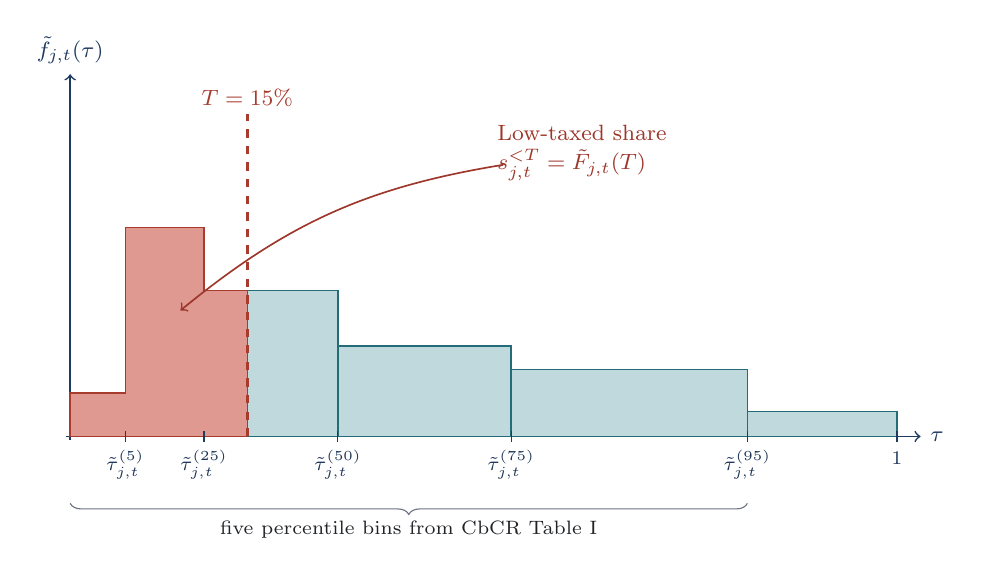
\begin{tikzpicture}[font=\small]
  % Coordinates: x in [0, 11], y in [0, 4.6]
  \def\pa{0.7}  % P5
  \def\pb{1.7}  % P25
  \def\pc{3.4}  % P50
  \def\pd{5.6}  % P75
  \def\pe{8.6}  % P95
  \def\Tx{2.25} % 15% threshold

  % Axes
  \draw[->, thesisNavy, line width=0.6pt] (-0.05,0) -- (10.8,0) node[right, font=\footnotesize] {$\tau$};
  \draw[->, thesisNavy, line width=0.6pt] (0,-0.05) -- (0,4.6) node[above, font=\footnotesize] {$\tilde{f}_{j,t}(\tau)$};

  % Piecewise rectangles (heights chosen so each bin's area equals percentile mass)
  \fill[thesisTeal!30, draw=thesisTeal!85!black, line width=0.5pt] (0,0) rectangle (\pa, 0.55);
  \fill[thesisTeal!30, draw=thesisTeal!85!black, line width=0.5pt] (\pa,0) rectangle (\pb, 2.65);
  \fill[thesisTeal!30, draw=thesisTeal!85!black, line width=0.5pt] (\pb,0) rectangle (\pc, 1.85);
  \fill[thesisTeal!30, draw=thesisTeal!85!black, line width=0.5pt] (\pc,0) rectangle (\pd, 1.15);
  \fill[thesisTeal!30, draw=thesisTeal!85!black, line width=0.5pt] (\pd,0) rectangle (\pe, 0.85);
  \fill[thesisTeal!30, draw=thesisTeal!85!black, line width=0.5pt] (\pe,0) rectangle (10.5, 0.32);

  % Highlight low-taxed area in red overlay
  \fill[thesisRed!55] (0,0) rectangle (\pa, 0.55);
  \fill[thesisRed!55] (\pa,0) rectangle (\pb, 2.65);
  \fill[thesisRed!55] (\pb,0) rectangle (\Tx, 1.85);
  \draw[thesisRed!85!black, line width=0.5pt] (0,0) -- (0,0.55) -- (\pa,0.55) -- (\pa,2.65)
    -- (\pb,2.65) -- (\pb,1.85) -- (\Tx,1.85) -- (\Tx,0) -- cycle;

  % Threshold
  \draw[thesisRed!85!black, dashed, line width=0.9pt] (\Tx,0) -- (\Tx,4.1);
  \node[font=\footnotesize, thesisRed!85!black] at (\Tx,4.3) {$T = 15\%$};

  % Percentile ticks
  \foreach \x/\lbl in {\pa/{(5)}, \pb/{(25)}, \pc/{(50)}, \pd/{(75)}, \pe/{(95)}} {
    \draw[thesisNavy] (\x,0.07) -- (\x,-0.07);
    \node[below, font=\scriptsize, thesisNavy!90!black] at (\x,-0.05) {$\tilde{\tau}_{j,t}^{\lbl}$};
  }
  \draw[thesisNavy] (10.5, 0.07) -- (10.5, -0.07) node[below, font=\scriptsize] {$1$};

  % Annotation arrow & label for shaded mass
  \node[font=\footnotesize, align=left, thesisRed!80!black]
    at (6.5, 3.6) {Low-taxed share\\[1pt]$\displaystyle s^{<T}_{j,t} = \tilde{F}_{j,t}(T)$};
  \draw[thesisRed!80!black, ->, line width=0.6pt] (5.5,3.45) to[bend right=15] (1.4, 1.6);

  % Bracket below x-axis showing rising/decreasing CDF mass
  \draw[decorate, decoration={brace, mirror, amplitude=4pt}, thesisGrey]
    (0,-0.85) -- node[below=3pt, font=\scriptsize, thesisGrey!30!black]
    {five percentile bins from CbCR Table I} (\pe,-0.85);
\end{tikzpicture}
\caption[Piecewise-uniform ETR distribution with zero-extended lower tail.]{Mixed continuous--discrete ETR distribution fitted to the five jurisdiction-level percentiles from CbCR Table I (equations \ref{eq:mixture}--\ref{eq:piecewise}). The lower-tail rectangle spans $[0, \tilde{\tau}^{(5)}]$ with mass $0.05$; the four interior rectangles are the uniform components (masses $0.20, 0.25, 0.25, 0.20$) on the supports between adjacent percentiles; each rectangle's height is its mass divided by its bin width, so that areas integrate to the stated component masses. The upper point mass ($0.05$ at $\tilde{\tau}^{(95)}$) is not drawn separately, it appears as a vertical jump in the CDF rather than as a finite density value. The red shading marks the low-taxed mass $s^{<T}_{j,t}$ (equation \ref{eq:lowtax_share}). The bin straddling $T = 15\%$ is split by linear interpolation of the uniform CDF. The departure from \citet{hugger2026}, who place a point mass at $\tilde{\tau}^{(5)}$, is that the lower-tail component here admits a well-defined density at every ETR between zero and $\tilde{\tau}^{(5)}$, preserving the mathematical existence of near-zero-ETR profit in the Stage-1 segment.}
\label{fig:piecewise_uniform}
\end{figure}

\subsubsection{Hybrid measurement and cross-validation against Table IV}\label{sec:crossval}

The distributional fit \eqref{eq:lowtax_share} and the direct Table IV observation are complementary data objects. Table IV reports the actual profit mass inside the $[0, 15\%)$ bracket at subsidiary level but covers only 49 parent jurisdictions and 154 affiliate jurisdictions (Section \ref{sec:t4_main}). Table I covers 58 parent and 240 affiliate jurisdictions but only through five aggregated percentiles. For every $(j, t)$ cell, the hybrid Stage 1 measurement uses the most informative source actually observed:
\begin{equation}\label{eq:hybrid}
s_{j,t}^{<T,\text{hyb}} = \begin{cases}
\dfrac{\pi_{j,t}^{<T,\text{IV}}}{\pi_{j,t}^{\text{all,IV}}} & \text{if Table IV is observed for cell } (j, t), \\[8pt]
\tilde{F}_{j,t}(T) \text{ from eq. \eqref{eq:lowtax_share}} & \text{if only Table I percentiles are observed,} \\[4pt]
\mathbb{1}\!\{\bar{\tau}_{j,t} < T\} & \text{if neither is observed.}
\end{cases}
\end{equation}
Profit volumes inside Table IV brackets use the corrected profit base $\pi^{*}$ wherever \code{PROFIT\_ADJ} is observed; where only \code{PROFIT} is available, the correction ratio $\hat{\gamma}_{j,t}$ from equation \eqref{eq:correction_model} is applied. All 27 EU Member States appear as affiliate jurisdictions in Table IV across the 2016--2022 vintages, so the first branch of \eqref{eq:hybrid} covers the entire EU sample and the second branch is reserved for the non-EU extension of the revenue pipeline. The bilateral low-taxed profit volume used by the rest of the pipeline is:
\begin{equation}\label{eq:lowtax_profit}
\ell_{p,j,t} = s_{j,t}^{<T,\text{hyb}} \cdot \pi_{p,j,t}^{*}.
\end{equation}
Table IV also reports business-activity counts inside the \code{RATE\_0-15} bracket (\code{ACT\_HOLDING}, \code{ACT\_IP}, \code{ACT\_MAN}). These do not enter \eqref{eq:hybrid} directly but diagnose whether the low-taxed profit in a given cell is dominated by conduit or operating entities, which is the input Section \ref{sec:sbie_decomp} needs to decide whether the aggregate SBIE ratio overstates or understates shielding.

Three tests are run on the overlapping sample. First, for each $(j, t)$ cell observed in both tables, the low-taxed share from Table I (equation \ref{eq:lowtax_share}) is compared against the Table IV direct share. A Wilcoxon signed-rank test assesses $H_0\colon \text{median}(s^{<T,\text{I}} - s^{<T,\text{IV}}) = 0$. It is preferred over a paired $t$-test because the differences are bounded on $[-1, 1]$ and will not be normally distributed. A systematic positive difference indicates that the Hugger fit overstates the low-taxed share, plausible if the tail point masses are placed too low. A negative difference indicates compression of bimodality.

Second, Table IV reports profit volumes in discrete ETR brackets (\code{RATE\_0-15}, \code{RATE\_15}, \code{RATE\_20-30}, \code{RATE\_30}, and the negative-profit categories). Integrating the Table I mixture CDF \eqref{eq:piecewise} across bracket boundaries produces a predicted profit share for each bracket. For each $(j, t)$ cell the fit is measured by the total variation distance:
\begin{equation}\label{eq:chisq_crossval}
\text{TV}_{j,t} = \tfrac{1}{2}\sum_{b=1}^{B} \left|\hat{\omega}_{j,t,b}^{\text{I}} - \omega_{j,t,b}^{\text{IV}}\right|,
\end{equation}
where $\omega_{j,t,b}^{\text{IV}}$ is the observed profit share in bracket $b$ and $\hat{\omega}_{j,t,b}^{\text{I}}$ is the Table I prediction.\footnote{Total variation is preferred to a chi-square metric because the objects being compared are profit shares (bounded on $[0, 1]$, potentially zero in empty brackets), not multinomial counts with a natural denominator. $\text{TV}_{j,t} \in [0, 1]$ has a direct interpretation as the minimum share of mass that must be reallocated across brackets to match the observed distribution.} High-$\text{TV}_{j,t}$ cells are flagged and their concentration in conduit jurisdictions versus the broader EU indicates whether the approximation error is structural (bimodality-driven) or idiosyncratic.

Third, point-estimate error and distributional error only matter if they translate into revenue bias. For each cell in the overlap I compute two Stage 1 revenue estimates (Table I and IV) holding all other pipeline stages constant. The percentage revenue difference is regressed on the within-jurisdiction ETR interquartile range from Table I:
\begin{equation}\label{eq:crossval_regression}
\frac{R_{j,t}^{\text{I}} - R_{j,t}^{\text{IV}}}{R_{j,t}^{\text{IV}}} = \alpha + \delta \cdot \text{IQR}_{j,t}^{\text{ETR}} + \gamma_t + \varepsilon_{j,t},
\end{equation}
where $\gamma_t$ are year fixed effects absorbing vintage changes in CbCR coverage. $\hat{\delta}$ tests whether greater within-jurisdiction ETR dispersion also predicts measurement error in the distributional approach. A significant $\hat{\delta}$ provides a correction factor $\hat{\alpha} + \hat{\delta} \cdot \text{IQR}$ that can be applied to Table I estimates for non-EU jurisdictions where Table IV is unavailable. If $\hat{\delta}$ is close to zero, the distributional approach is approximately unbiased and the hybrid design \eqref{eq:hybrid} is a conservative refinement. If $\hat{\delta}$ is large, the non-EU extension must be interpreted as a lower bound wherever Table I IQR is high.

\subsection{Stage 2: Substance-based income exclusion}\label{sec:SBIE}

The second pipeline stage determines what fraction of low-taxed profit generates a top-up tax liability. The SBIE shields a proportion of profit by excluding returns to tangible assets and payroll. \citet{devereux2023} find an average SBIE-to-profit ratio of 57\% at initial carve-out rates, so only 43\% of GloBE income constitutes excess profit subject to the top-up tax.

\subsubsection{The effective tax floor under Pillar Two}\label{sec:floor}

The total tax on an MNE subsidiary in a low-tax jurisdiction ($\tau_{p,j} < T$) with positive excess profit is:
\begin{equation}\label{eq:total_tax}
\text{Tax} = \underbrace{\tau_{p,j} \cdot \pi_{p,j}}_{\text{local CIT}} + \underbrace{(T - \tau_{p,j}) \cdot (\pi_{p,j} - \text{SBIE}_{p,j})}_{\text{top-up tax}}
\end{equation}

The effective tax rate under the Global Minimum Tax is: 
\begin{equation}\label{eq:etr_pillar2}
\tau_{p,j}^{\text{P2}} = T - (T - \tau_{p,j}) \cdot \frac{\text{SBIE}_{p,j}}{\pi_{p,j}} = T - \delta_{p,j}^{\text{top}} \cdot \phi_{p,j}
\end{equation}
\begin{figure}[H]
\centering
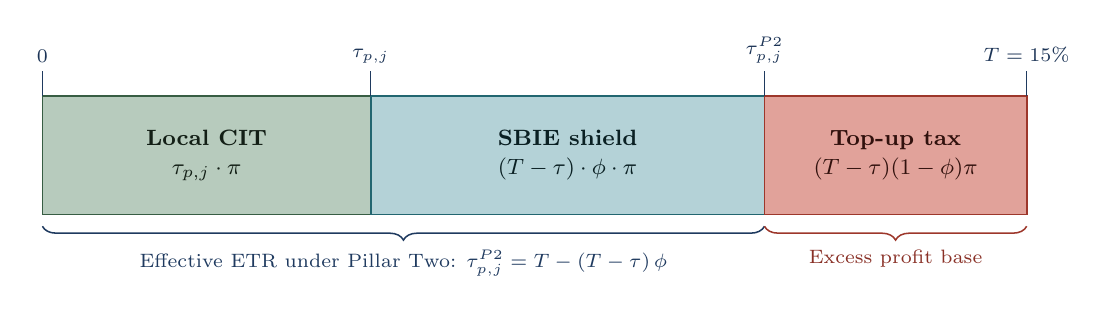
\begin{tikzpicture}[font=\small]
  % Bar dimensions
  \def\W{12.5}
  \def\H{1.5}
  % Sub-widths (proportional to a scenario with tau = 5% of profit-base, T = 15%, phi = 0.6)
  % local CIT = tau/T part of total potential tax = 5/15 = 1/3 of bar
  % gap = (T-tau) = 10/15 = 2/3 of bar; of which phi=0.6 → SBIE shielded; (1-phi)=0.4 → top-up
  % Use proportional widths: local CIT = 4.17 cm, SBIE = 5.0 cm, top-up = 3.33 cm  (sums to 12.5)
  \def\xa{4.17}
  \def\xb{9.17}

  % Background
  \fill[thesisLight] (0,0) rectangle (\W,\H);

  % Local CIT
  \fill[thesisGreen!40, draw=thesisGreen!75!black, line width=0.6pt] (0,0) rectangle (\xa, \H);
  \node[font=\footnotesize, align=center, thesisGreen!25!black]
    at (\xa/2, \H/2) {\textbf{Local CIT}\\[1pt]$\tau_{p,j}\cdot\pi$};

  % SBIE shield
  \fill[thesisTeal!35, draw=thesisTeal!80!black, line width=0.6pt] (\xa,0) rectangle (\xb, \H);
  \node[font=\footnotesize, align=center, thesisTeal!25!black]
    at ({(\xa+\xb)/2}, \H/2) {\textbf{SBIE shield}\\[1pt]$(T-\tau)\cdot\phi\cdot\pi$};

  % Top-up tax
  \fill[thesisRed!50, draw=thesisRed!80!black, line width=0.6pt] (\xb,0) rectangle (\W, \H);
  \node[font=\footnotesize, align=center, thesisRed!25!black]
    at ({(\xb+\W)/2}, \H/2) {\textbf{Top-up tax}\\[1pt]$(T-\tau)(1-\phi)\pi$};

  % Top axis with markers
  \draw[thesisNavy, line width=0.5pt] (0, \H) -- (0, \H+0.32);
  \draw[thesisNavy, line width=0.5pt] (\xa, \H) -- (\xa, \H+0.32);
  \draw[thesisNavy, line width=0.5pt] (\xb, \H) -- (\xb, \H+0.32);
  \draw[thesisNavy, line width=0.5pt] (\W, \H) -- (\W, \H+0.32);
  \node[above, font=\scriptsize, thesisNavy!90!black] at (0, \H+0.30) {$0$};
  \node[above, font=\scriptsize, thesisNavy!90!black] at (\xa, \H+0.30) {$\tau_{p,j}$};
  \node[above, font=\scriptsize, thesisNavy!90!black] at (\xb, \H+0.30) {$\tau^{P2}_{p,j}$};
  \node[above, font=\scriptsize, thesisNavy!90!black] at (\W, \H+0.30) {$T = 15\%$};

  % Effective P2 brace
  \draw[decorate, decoration={brace, mirror, amplitude=5pt}, thesisNavy, line width=0.55pt]
    (0,-0.15) -- node[below=5pt, font=\scriptsize]
    {Effective ETR under Pillar Two: $\tau^{P2}_{p,j} = T - (T-\tau)\,\phi$} (\xb,-0.15);

  % Top-up brace
  \draw[decorate, decoration={brace, mirror, amplitude=5pt}, thesisRed!80!black, line width=0.55pt]
    (\xb,-0.15) -- node[below=5pt, font=\scriptsize, thesisRed!70!black] {Excess profit base} (\W,-0.15);
\end{tikzpicture}
\caption[Effective Pillar Two tax floor.]{Decomposition of taxable profit at the 15\% threshold for a low-tax MNE affiliate. Local corporate income tax (green) collects $\tau_{p,j}\cdot\pi$. The SBIE (teal) shields a fraction $\phi=\text{SBIE}/\pi$ of the gap to the headline rate, leaving only the residual (red) as the excess profit base on which the top-up tax of $(T-\tau)(1-\phi)\pi$ is levied. The Pillar Two effective tax rate $\tau^{P2}_{p,j}$ therefore lies strictly below the headline 15\% whenever physical substance is positive, with the gap widening for capital- and labour-intensive sectors.}
\label{fig:effective_floor}
\end{figure}

where $\phi_{p,j} \equiv \text{SBIE}_{p,j} / \pi_{p,j}$ is the SBIE-to-profit ratio.\footnote{The $\phi$ notation for the SBIE-to-profit ratio is introduced in this thesis. \citet{devereux2023} compute the ratio but do not assign it a symbol; \citet{schjelderup2024} work with absolute SBIE values. The ratio formulation makes the effective floor directly comparable across jurisdictions with different profit levels. The symbol $\phi$ is chosen to avoid confusion with $\rho$, which conventionally denotes a correlation coefficient in econometric reporting.} The effective tax rate under Pillar Two falls \emph{strictly below} the headline rate $T = 15\%$ whenever the SBIE is positive. The gap is larger when the pre-reform ETR is further below 15\% (larger $\delta^{\text{top}}$) and the SBIE-to-profit ratio is larger (larger $\phi$).

The SBIE for each bilateral pair is:
\begin{equation}\label{eq:sbie}
\text{SBIE}_{p,j,t} = \sigma_W(t) \cdot \hat{W}_{p,j,t} + \sigma_A(t) \cdot A_{p,j,t}
\end{equation}
The carve-out rates decline linearly over a ten-year transition period (2024--2033). The payroll carve-out $\sigma_W$ starts at 10\% in 2024 and falls by 0.5 percentage points per year to reach 5\% from 2033 onward. The tangible asset carve-out $\sigma_A$ starts at 8\% in 2024 and falls by approximately 0.3 percentage points per year to reach 5\% from 2033 onward. The factorial design estimates revenue at both endpoints of this transition. Factor 3 switches between initial carve-out rates ($\sigma_W = 0.10$, $\sigma_A = 0.08$) and long-run rates ($\sigma_W = \sigma_A = 0.05$).

The payroll component $\hat{W}_{p,j,t}$ uses observed \code{EARNINGS} where available; where missing, it is imputed as $N_{p,j,t} \times \bar{w}_{j,t}$ using employee counts and jurisdiction-average wages.\label{sec:payroll_imputation}

\subsubsection{SBTI Safe Harbour amplification}\label{sec:sbti_amplification}\label{sec:sbti}

The January 2026 OECD Administrative Guidance introduced the Substance-Based Tax Incentive (SBTI) Safe Harbour, which creates a second channel through which physical substance reduces the GMT burden \citep{oecd2026}. Under the original GloBE rules, local tax credits mechanically reduced covered taxes, driving the ETR below 15\% and triggering a top-up tax. The SBTI reverses this: MNEs may treat ``Qualifying Tax Incentives'' (QTIs; expenditure-based R\&D credits, volume-based production incentives) as an addition to covered taxes rather than a reduction. By inflating the ETR numerator, the safe harbour prevents the ETR from being artificially depressed.\footnote{The original GloBE design intended covered taxes to reflect the actual tax burden. Tax credits, even those designed to incentivise real economic activity, mechanically reduced covered taxes below the amount the jurisdiction intended the MNE to pay. The SBTI corrects this misalignment by treating qualifying incentives as additions to rather than reductions of covered taxes, preserving the incentive the source country offered.}

The benefit is bounded by a Substance Cap, for which two methods are available \citep{oecd2026}. Under Method 1 (the default, permanent option), the cap equals 5.5\% of the greater of eligible payroll costs or depreciation and depletion of eligible tangible assets:
\begin{equation}\label{eq:substance_cap}
\text{SC}_{p,j,t}^{\text{M1}} = 0.055 \times \max\!\left(W_{p,j,t},\; \text{Depr}(A_{p,j,t})\right)
\end{equation}
where $\text{Depr}(A)$ denotes depreciation and depletion of eligible tangible assets. Under Method 2 (an elective alternative available for a five-year period), the cap equals 1\% of the carrying value of eligible tangible assets:
\begin{equation}\label{eq:substance_cap_m2}
\text{SC}_{p,j,t}^{\text{M2}} = 0.01 \times A_{p,j,t}
\end{equation}
MNEs elect whichever method yields the larger cap. Method 2 is designed for incentives linked to initial capital expenditure, where the carrying value provides greater relief in early years of asset life than depreciation.\footnote{If an MNE revokes a Method 2 election, assets previously included under Method 2 must be excluded from the depreciation calculation under Method 1, preventing double benefit. See \citet{oecd2026}, Chapter 1, Section 4.}

The SBTI and the SBIE rely on the \emph{same} macroeconomic variables: payroll and tangible assets. The SBIE reduces the denominator of the excess profit base; the SBTI inflates the numerator of the ETR. Capital-intensive sectors benefit doubly: larger SBIE carve-outs \emph{and} higher Substance Caps, allowing them to retain local tax incentives without triggering top-up taxes. Asset-light holding companies in conduit jurisdictions cannot utilise the SBTI because their payroll and tangible assets approach zero, driving the Substance Cap to zero.\footnote{The SBTI also has implications for tax competition. As \citet{janeba2023} predict, competition shifts from headline statutory rates toward opaque subsidies and qualified refundable tax credits. The SBTI explicitly protects expenditure-based incentives up to the Substance Cap, restricting effective tax competition to jurisdictions with heavy industrial footprints.}

Under the SBTI, the effective ETR becomes:
\begin{equation}\label{eq:etr_sbti}
\tau_{p,j}^{\text{SBTI}} = \frac{\theta_{p,j} + \min\!\left(\text{QTI}_{p,j},\; \max\!\left(\text{SC}_{p,j}^{\text{M1}},\; \text{SC}_{p,j}^{\text{M2}}\right)\right)}{\pi_{p,j}}
\end{equation}
where the MNE elects the method that yields the larger cap.

Public CbCR does not observe actual QTI claims. The methodology therefore cannot measure the SBTI benefit directly but can measure how much \emph{room} a jurisdiction--sector cell has to protect local tax incentives under the safe harbour. The Substance Cap sets the upper bound on the SBTI benefit; the SBTI-capacity proxy normalises this cap by profit to obtain a ratio comparable across jurisdictions and sectors:
\begin{equation}\label{eq:sbti_capacity}
\kappa_{j,s,t} = \frac{\max\!\left(0.055\,W_{j,s,t},\; 0.01\,A_{j,s,t}\right)}{\pi_{j,s,t}}
\end{equation}
The numerator approximates the maximum Substance Cap an MNE could claim by combining the most favourable observable component from each method. Under Method 1, the cap is $0.055 \times \max(W, \text{Depr}(A))$; however, CbCR reports the carrying value of tangible assets (\code{ASSETS}) but not depreciation, so the Method 1 asset arm ($0.055 \times \text{Depr}(A)$) cannot be computed from public data. The proxy therefore takes the maximum of the Method 1 payroll arm ($0.055 \times W$, which is observable) and the Method 2 carrying-value cap ($0.01 \times A$, also observable). This yields a conservative upper bound: MNEs will elect whichever method produces the larger cap, and the proxy captures the larger of the two observable components. A high $\kappa$ indicates that a sector has substantial physical substance relative to profits and could therefore protect a large share of local tax incentives through the SBTI; a low $\kappa$ (characteristic of asset-light holding and IP licensing sectors) means the Substance Cap approaches zero and the SBTI provides little relief. The index enters the factorial design as part of the substance overlay in Factor 2 (Section \ref{sec:factors}).

\subsubsection{Sectoral decomposition}\label{sec:sbie_decomp}

The aggregate SBIE-to-profit ratio $\phi$ masks substantial sectoral heterogeneity. Manufacturing subsidiaries have high payroll and tangible asset intensity relative to profits, generating SBIE ratios that can exceed 100\% of pre-tax profit; holding and IP licensing entities have near-zero substance, driving the SBIE toward zero \citep{devereux2023}. Since the GMT applies the top-up tax at the entity level, the aggregate $\phi$ overstates shielding for jurisdictions where low-taxed profit is concentrated in asset-light entities. The sectoral decomposition combines CbCR aggregate levels with the Eurostat FATS sectoral shares introduced in Section \ref{sec:fats_main}.

The SBIE-to-profit ratio $\phi$ depends on the composition of economic activity. Decomposing affiliates in jurisdiction $j$ into sectors $s \in \{1, \ldots, S\}$:

\begin{equation}\label{eq:rho_sectoral}
\phi_j = \sum_s \omega_{j,s} \cdot \phi_{j,s}, \quad \text{where } \omega_{j,s} = \frac{\pi_{j,s}}{\pi_j}
\end{equation}

and the sector-specific SBIE-to-profit ratio is:
\begin{equation}\label{eq:rho_sector}
\phi_{j,s} = \sigma_W \cdot \frac{W_{j,s}}{\pi_{j,s}} + \sigma_A \cdot \frac{A_{j,s}}{\pi_{j,s}}
\end{equation}

The effective tax floor for sector $s$ in jurisdiction $j$ is:
\begin{equation}\label{eq:floor_sector}
\tau_{j,s}^{\text{floor}} = T - (T - \tau_j) \cdot \phi_{j,s}
\end{equation}

CbCR does not report by sector. The sectoral decomposition combines CbCR aggregate levels with Eurostat FATS sectoral shares:
\begin{equation}\label{eq:sbie_sectoral}
\widehat{\text{SBIE}}_{j,s} = \sigma_W \cdot \left(\frac{\text{PersC}_{j,s}^{\text{FATS}}}{\sum_{s'} \text{PersC}_{j,s'}^{\text{FATS}}}\right) \cdot W_j^{\text{CbCR}} + \sigma_A \cdot \left(\frac{\hat{K}_{j,s}}{\sum_{s'} \hat{K}_{j,s'}}\right) \cdot A_j^{\text{CbCR}}
\end{equation}
\begin{figure}[H]
\centering
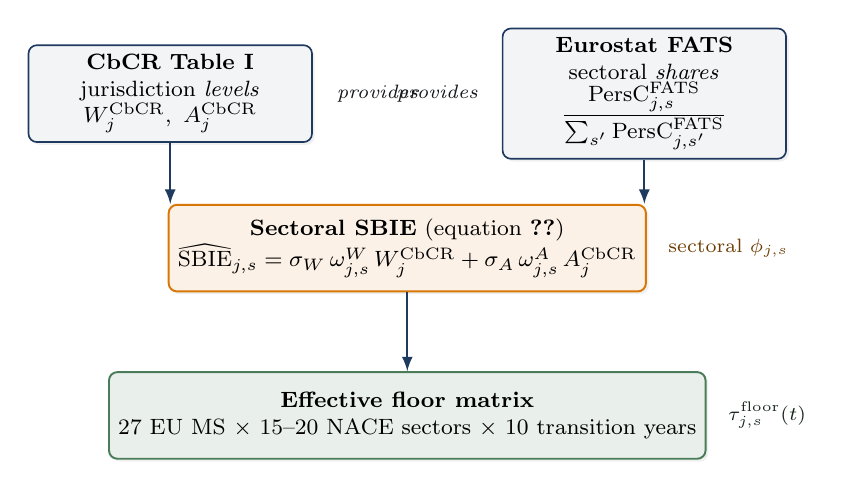
\begin{tikzpicture}[font=\small,
   src/.style={draw=thesisNavy, line width=0.6pt, rounded corners=3pt, fill=thesisLight,
               minimum width=3.6cm, minimum height=1.0cm, align=center, font=\footnotesize,
               drop shadow={shadow xshift=1pt, shadow yshift=-1pt, opacity=0.12}},
   prod/.style={draw=thesisOrange, line width=0.7pt, rounded corners=3pt,
                fill=thesisOrange!10, minimum width=4.6cm, minimum height=1.1cm,
                align=center, font=\footnotesize,
                drop shadow={shadow xshift=1pt, shadow yshift=-1pt, opacity=0.12}}]

  % Top row: sources
  \node[src] (cbcr) {\textbf{CbCR Table I}\\jurisdiction \emph{levels}\\$W^{\text{CbCR}}_j,\ A^{\text{CbCR}}_j$};
  \node[src, right=2.4cm of cbcr] (fats) {\textbf{Eurostat FATS}\\sectoral \emph{shares}\\$\dfrac{\text{PersC}^{\text{FATS}}_{j,s}}{\sum_{s'}\text{PersC}^{\text{FATS}}_{j,s'}}$};

  % Middle: combine box
  \node[prod, below=1.4cm of $(cbcr)!0.5!(fats)$] (combine)
    {\textbf{Sectoral SBIE} (equation \ref{eq:sbie_sectoral})\\
     $\widehat{\text{SBIE}}_{j,s}
        = \sigma_W\,\omega^{W}_{j,s}\,W^{\text{CbCR}}_j
        + \sigma_A\,\omega^{A}_{j,s}\,A^{\text{CbCR}}_j$};

  % Bottom: matrix output
  \node[prod, below=1.0cm of combine, fill=thesisGreen!12, draw=thesisGreen] (out)
    {\textbf{Effective floor matrix}\\
     27 EU MS\ \(\times\)\ 15--20 NACE sectors\ \(\times\)\ 10 transition years};

  % Arrows
  \draw[thesis arrow] (cbcr.south) -- ($(combine.north -| cbcr.south)$);
  \draw[thesis arrow] (fats.south) -- ($(combine.north -| fats.south)$);
  \draw[thesis arrow] (combine) -- (out);

  % Side annotations
  \node[font=\scriptsize\itshape, thesisGrey!20!black, anchor=west] at ($(cbcr.east) + (0.18,0)$) {provides};
  \node[font=\scriptsize\itshape, thesisGrey!20!black, anchor=east] at ($(fats.west) + (-0.18,0)$) {provides};
  \node[font=\scriptsize, thesisOrange!50!black, anchor=west] at ($(combine.east) + (0.15,0)$)
    {sectoral $\phi_{j,s}$};
  \node[font=\scriptsize, thesisGreen!30!black, anchor=west] at ($(out.east) + (0.15,0)$)
    {$\tau^{\text{floor}}_{j,s}(t)$};

\end{tikzpicture}
\caption[CbCR$\,\times\,$FATS construction of sectoral SBIE.]{Construction of the sectoral SBIE and the effective tax floor matrix. CbCR Table I provides the in-scope MNE \emph{levels} of payroll and tangible assets for each affiliate jurisdiction; Eurostat FATS provides the cross-sectoral \emph{shares} within each jurisdiction (NACE-level personnel costs and imputed capital stock). Their combination yields a sector-specific SBIE estimate $\widehat{\text{SBIE}}_{j,s}$ (equation \ref{eq:sbie_sectoral}), from which the effective tax floor $\tau^{\text{floor}}_{j,s}(t)$ is computed for each year of the SBIE transition.}
\label{fig:cbcr_fats_combo}
\end{figure}

where $\text{PersC}_{j,s}^{\text{FATS}}$ is the personnel costs for sector $s$ in FATS and $\hat{K}_{j,s}$ is imputed tangible assets. FATS provides the \emph{sectoral shares}; CbCR provides the \emph{aggregate levels}. The CbCR in-scope population (\EUR750 million+ MNEs) is a subset of the FATS population (all foreign-controlled enterprises), so using FATS shares on CbCR totals is conservative.\footnote{FATS does not report tangible assets directly. The tangible asset share is imputed from the capital intensity (investment-to-turnover ratio) of each NACE sector, using FATS investment data where available and EU KLEMS capital stock data as a cross-check. This imputation is the weakest link in the sectoral decomposition.}

The Eurostat inward FATS underwent a structural break in 2021: the pre-2021 series (\code{fats\_g1b\_08}) uses a single broad aggregate and 23 indicators, while the post-2021 series (\code{fats\_activ}) uses 48 NACE-based activity categories and 19 \code{indic\_sbs} codes. The sectoral estimation therefore uses post-2021 \code{fats\_activ} data only.

The effective tax floor evolves over the SBIE transition period (2024--2033):
\begin{equation}\label{eq:floor_transition}
\tau_{j,s}^{\text{floor}}(t) = T - (T - \tau_j) \cdot \left[\sigma_W(t) \cdot \frac{W_{j,s}}{\pi_{j,s}} + \sigma_A(t) \cdot \frac{A_{j,s}}{\pi_{j,s}}\right]
\end{equation}
The output is a matrix of effective tax floors: 27 EU Member States $\times$ 15--20 NACE sectors $\times$ 10 transition years.

For jurisdictions where the ETR distribution straddles $T$, the aggregate $\phi_j$ overstates the effective shielding of the GMT base if high-ETR entities are disproportionately capital-intensive. The SBIE reduces the top-up tax only on the low-taxed portion, not on entities already above $T$. Table IV's activity composition variables (\code{ACT\_HOLDING}, \code{ACT\_IP}, \code{ACT\_MAN}) for the \code{RATE\_0-15} bracket reveal whether low-taxed profit is concentrated in holding/IP activities (low $\phi$, suggesting proportional SBIE allocation \emph{overstates} shielding) or in manufacturing (high $\phi$, suggesting it \emph{understates} shielding). The sensitivity analysis tests both extremes.

Stage 2 delivers the SBIE filter $(1 - \bar{\phi}_{p,j,t})$: the fraction of low-taxed profit that constitutes excess profit and is subject to the top-up tax. The factorial design varies this filter through two factors: Factor 2 switches between the aggregate CbCR-based $\phi$ and the sectoral FATS-based $\phi$ with SBTI-capacity overlay, and Factor 3 switches between initial and long-run carve-out rates.

\subsection{Panel estimation of profit-shifting semi-elasticities}\label{sec:estimation}

The preceding stages identify low-taxed profit and compute the SBIE shield. Before modelling the behavioural response, this section estimates the key behavioural parameter, the tax semi-elasticity of reported profits, directly from the 2016--2022 CbCR panel. Published semi-elasticities are estimated either from US-only data \citep{dowd2017} or from a single cross-section of OECD CbCR \citep{garcia-bernardo2024}. The panel structure of this thesis provides two identification advantages: within-pair variation across seven fiscal years, which absorbs time-invariant bilateral confounders, and sufficient degrees of freedom to compare functional forms with formal specification tests rather than visual inspection.

\subsubsection{Estimation framework}\label{sec:hines_rice}

The estimation follows the Hines--Rice framework \citep{hines1994}, as extended by \citet{garcia-bernardo2024}. Reported pre-tax profit in affiliate jurisdiction $j$ of parent $p$ in year $t$ is modelled as a function of real economic activity and the tax incentive to shift profits:
\begin{equation}\label{eq:panel_linear}
\log \pi_{p,j,t}^{*} = \beta_0 + \beta_1 \log A_{p,j,t} + \beta_2 \log \hat{W}_{p,j,t} + \beta_3 \, \tau_{p,j,t} + \mathbf{\beta}_x \mathbf{X}_{p,j,t} + \alpha_{pj} + \gamma_t + \varepsilon_{p,j,t}
\end{equation}
where $\pi^{*}$ is corrected profit (equation \ref{eq:correction_model}), $A$ is tangible assets, $\hat{W}$ is payroll (observed or imputed), $\tau$ is the effective tax rate, $\alpha_{pj}$ is a parent--affiliate pair fixed effect, and $\gamma_t$ is a year fixed effect. The vector $\mathbf{X}$ contains log GDP per capita and log population of the affiliate jurisdiction.\footnote{Tangible assets $A$ are themselves affected by profit shifting: US MNEs in Luxembourg report the second-highest value of tangible assets in Europe \citep{garcia-bernardo2024}. Using tangible assets as a control therefore produces conservative semi-elasticity estimates, since part of the profit-shifting effect is absorbed by the capital stock. An instrumental variable strategy using lagged assets is explored as a robustness check (Section \ref{sec:estimation_robustness}).} The coefficient $\beta_3$ is the linear semi-elasticity: the percentage change in reported profits for a one percentage-point change in the ETR.\footnote{The bilateral pair fixed effects $\alpha_{pj}$ absorb all time-invariant determinants of bilateral profit allocation: treaty networks, geographic and linguistic proximity, legal system similarity, and persistent features of MNE group structure. Identification of $\beta_3$ therefore comes from \emph{within-pair} variation in ETRs over 2016--2022, driven by domestic tax reforms, changes in the composition of reporting entities, and shifts in the profit base. Year fixed effects absorb global shocks (the 2017 TCJA, the 2020 COVID contraction, and the post-2020 recovery).}

The linear specification restricts the semi-elasticity to be constant across the ETR distribution. Two nonlinear extensions relax this:

\textit{Quadratic specification.} Following \citet{dowd2017}:
\begin{equation}\label{eq:panel_quadratic}
\log \pi_{p,j,t}^{*} = \beta_0 + \beta_1 \log A_{p,j,t} + \beta_2 \log \hat{W}_{p,j,t} + \beta_3 \, \tau_{p,j,t} + \beta_4 \, \tau_{p,j,t}^2 + \mathbf{\beta}_x \mathbf{X}_{p,j,t} + \alpha_{pj} + \gamma_t + \varepsilon_{p,j,t}
\end{equation}
The implied semi-elasticity varies with the ETR: $\varepsilon(\tau) = \beta_3 + 2\beta_4 \tau$.

\textit{Logarithmic specification.} Following \citet{garcia-bernardo2024}:
\begin{equation}\label{eq:panel_log}
\log \pi_{p,j,t}^{*} = \beta_0 + \beta_1 \log A_{p,j,t} + \beta_2 \log \hat{W}_{p,j,t} + \beta_3 \, \tau_{p,j,t} + \beta_4 \log(t_0 + \tau_{p,j,t}) + \mathbf{\beta}_x \mathbf{X}_{p,j,t} + \alpha_{pj} + \gamma_t + \varepsilon_{p,j,t}
\end{equation}
where $t_0$ is a small offset parameter selected by minimising the BIC over the grid $t_0 \in [0.001, 0.200]$.\footnote{The offset $t_0$ prevents the logarithm from diverging at $\tau = 0$ and governs how steeply the semi-elasticity rises at very low ETRs. \citet{garcia-bernardo2024} report $t_0 = 0.0023$ based on the 2017 CbCR panel. The panel estimate may differ because the time dimension introduces additional variation at the tails.} The implied semi-elasticity is $\varepsilon(\tau) = \beta_3 + \beta_4 / (t_0 + \tau)$, which rises sharply as $\tau \to 0$. This is the key feature that captures extreme profit shifting at near-zero ETRs.\footnote{The logarithmic specification implies that the semi-elasticity becomes unbounded as $\tau \to 0$. In the revenue simulation, this is bounded by the data: the lowest observed ETR percentile (P5) provides a natural floor. Counterfactual profit changes are winsorised at the 99th percentile of the estimated $\hat{\beta}_{j,t}$ distribution to prevent a small number of cells with near-zero P5 from dominating the aggregate.}

\begin{figure}[H]
\centering
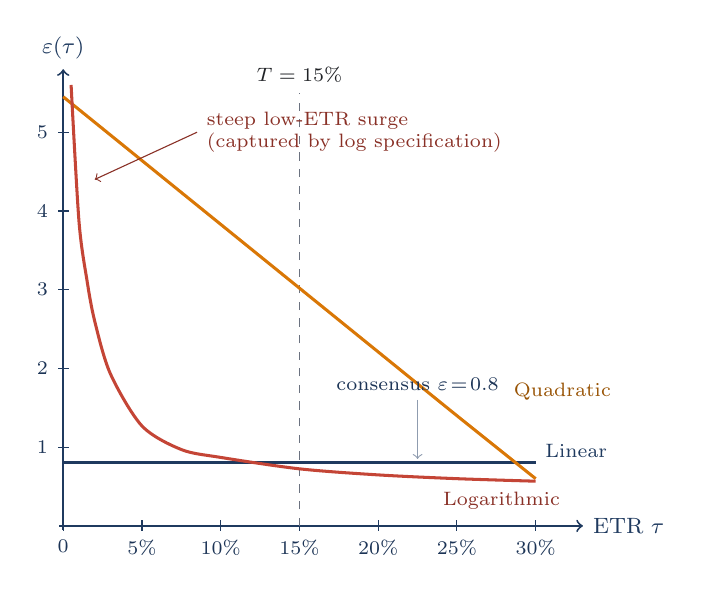
\begin{tikzpicture}[font=\small]
  % Coordinate system: x = tau in [0,30%]; we map x*20cm so 0.30 -> 6cm
  % y = semi-elasticity in [0, 5.5]; we map y*1cm
  \def\xmax{6.6}
  \def\ymax{5.8}

  % Axes
  \draw[->, thesisNavy, line width=0.7pt] (-0.05,0) -- (\xmax,0) node[right, font=\footnotesize] {ETR $\tau$};
  \draw[->, thesisNavy, line width=0.7pt] (0,-0.05) -- (0,\ymax) node[above, font=\footnotesize] {$\varepsilon(\tau)$};

  % x ticks (5% intervals)
  \foreach \xv/\lbl in {0/0, 1/{5\%}, 2/{10\%}, 3/{15\%}, 4/{20\%}, 5/{25\%}, 6/{30\%}} {
    \draw[thesisNavy] (\xv, 0.07) -- (\xv, -0.07);
    \node[below, font=\scriptsize, thesisNavy!90!black] at (\xv, -0.05) {\lbl};
  }
  % y ticks
  \foreach \yv in {1,2,3,4,5} {
    \draw[thesisNavy] (0.07, \yv) -- (-0.07, \yv);
    \node[left, font=\scriptsize, thesisNavy!90!black] at (-0.07, \yv) {\yv};
  }

  % T = 15% reference line
  \draw[dashed, thesisGrey, line width=0.6pt] (3, 0) -- (3, 5.5);
  \node[font=\scriptsize, thesisGrey!30!black, anchor=south] at (3, 5.5) {$T = 15\%$};

  % Linear: epsilon = 0.8
  \draw[thesisNavy, line width=1.1pt] (0, 0.8) -- (6, 0.8);
  \node[font=\scriptsize, thesisNavy, anchor=west] at (6.0, 0.95) {Linear};

  % Quadratic Dowd: epsilon(tau) = -10.73 + 16.178*(1 - tau)
  \draw[thesisOrange, line width=1.1pt]
    plot[smooth] coordinates {(0,5.45) (1,4.64) (2,3.83) (3,3.02) (4,2.21) (5,1.40) (6,0.60)};
  \node[font=\scriptsize, thesisOrange!70!black, anchor=west] at (5.6, 1.7) {Quadratic};

  % Logarithmic: epsilon(tau) = b3 + b4 / (t0 + tau) — illustrative parameters
  \draw[thesisRed, line width=1.1pt]
    plot[smooth] coordinates {(0.1,5.6) (0.2,3.87) (0.3,3.13) (0.4,2.6) (0.6,1.93)
      (1,1.27) (1.5,0.97) (2,0.87) (3,0.725) (4,0.648) (5,0.6) (6,0.568)};
  \node[font=\scriptsize, thesisRed!70!black, anchor=west] at (4.7, 0.32) {Logarithmic};

  % Annotation: meta-regression consensus
  \draw[thesisNavy!50, ->, line width=0.4pt] (4.5, 1.6) -- (4.5, 0.85);
  \node[font=\scriptsize, thesisNavy!90!black, anchor=south] at (4.5, 1.6) {consensus $\varepsilon\!=\!0.8$};

  % Annotation: nonlinear surge at low ETRs
  \draw[thesisRed!70!black, ->, line width=0.4pt] (1.7, 5) -- (0.4, 4.4);
  \node[font=\scriptsize, thesisRed!70!black, anchor=west, align=left] at (1.7, 5)
    {steep low-ETR surge\\(captured by log specification)};
\end{tikzpicture}
\caption[Implied semi-elasticity under three functional forms.]{Implied profit-shifting semi-elasticity $\varepsilon(\tau)$ under the three functional forms compared in Section \ref{sec:hines_rice}: the linear specification, equivalent to the meta-regression consensus of \citet{heckemeyer2017}; the quadratic specification of \citet{dowd2017} estimated on US administrative tax-return data; and the logarithmic specification of \citet{garcia-bernardo2024} estimated on a 2017 OECD CbCR cross-section. Coefficient values are illustrative; the panel-estimated values from Section \ref{sec:se_results} are reported in the results. The vertical dashed line marks the GMT threshold $T=15\%$. The logarithmic specification accommodates an unbounded surge in profit responsiveness as the ETR approaches zero, the regime in which the GMT base is concentrated.}
\label{fig:semi_elasticity_forms}
\end{figure}

\subsubsection{Identification}\label{sec:identification}

The pair fixed effects $\alpha_{pj}$ absorb all time-invariant bilateral determinants of profit allocation. Identification of the semi-elasticity coefficients ($\beta_3$, and $\beta_4$ where applicable) relies on within-pair changes in the effective tax rate over 2016--2022. Exogenous variation could be driven by domestic tax reforms in affiliate jurisdictions. Several EU Member States reduced their headline CIT rates during this period (e.g.\ France from 33.3\% to 25\%, Belgium from 33.99\% to 25\%). These rate changes induce variation in $\tau_{p,j,t}$ that is orthogonal to MNE-level profit-shifting decisions. Also, the 2017 US Tax Cuts and Jobs Act (TCJA) reduced the US federal CIT rate from 35\% to 21\% and introduced the GILTI regime, which altered the effective tax rate on US-parented foreign profits. This creates a discrete shift in the ETR of US--affiliate pairs. Lastly, as more jurisdictions adopted CbCR filing requirements (from 26 parent jurisdictions in 2016 to 49 in 2022), the sample expands. The pair fixed effects control for the level effect of new entrants; the concern is that entrants differ systematically in their ETR--profit relationship. A robustness check restricts the sample to the balanced panel of jurisdictions reporting in all seven years.

The sufficiency of within-pair ETR variation is an empirical question. Section \ref{sec:descriptive} reports the within-pair standard deviation of ETR. If the median within-pair standard deviation falls below 2 percentage points, the fixed-effects estimator may lack power relative to a specification that also uses between-pair variation. In that event, correlated random effects specification is estimated as an alternative: it augments the pooled regression with the pair-level mean of each time-varying regressor, so the coefficient on the demeaned regressor identifies the within-pair effect while the coefficient on the mean captures the between-pair effect.

\subsubsection{Inference}\label{sec:inference}

Standard errors are clustered at the affiliate-jurisdiction level to account for correlation across parent jurisdictions within the same affiliate (e.g.\ all MNEs operating in Ireland face correlated ETR shocks from Irish tax policy) .\footnote{Clustering at the affiliate level is more conservative than clustering at the pair level. An alternative two-way clustering (by parent and by affiliate) is reported as a robustness check. \citet{garcia-bernardo2024} use heteroscedasticity-robust standard errors on their cross-section; the panel structure requires cluster-robust inference .} Model selection proceeds in two stages. First, the BIC ranks the three functional forms. The BIC penalises model complexity more heavily than the AIC and is highly effective for comparing non-nested models with different numbers of parameters on the same sample. Second, because the quadratic and logarithmic specifications are non-nested (neither is a restricted case of the other), a \citet{vuong1989} test compares their observation-level log-likelihoods to determine whether one fits the data systematically better

\subsubsection{From estimated coefficients to the behavioural response}\label{sec:counterfactual}

The estimated coefficients $(\hat{\beta}_3, \hat{\beta}_4)$ and the implied semi-elasticity curve $\hat{\varepsilon}(\tau)$ feed into Stage 3, where they are mapped to a jurisdiction--year reallocation factor $\hat{\beta}_{j,t}$ via the closed-form counterfactual of equations \eqref{eq:cf_linear}--\eqref{eq:cf_log} and aggregated through \eqref{eq:beta_aggregated}.\footnote{The counterfactual holds tangible assets $A$ and payroll $\hat{W}$ at their pre-reform values. This is consistent with the evidence that real investment responds more slowly than profit allocation \citep{suarezserrato2018} and with the short- to medium-run horizon over which the semi-elasticity is identified. The second-round effect (SBIE shrinkage through reduced substance) is discussed in Section \ref{sec:benchmarks_unmodelled} but not modelled in the baseline.} Estimation uncertainty in $(\hat{\beta}_3, \hat{\beta}_4)$ propagates into the revenue estimates through a pairs cluster bootstrap (1{,}000 replications) that resamples affiliate-jurisdiction clusters; the procedure is detailed in Section \ref{sec:beta_uncertainty} together with the functional-form and extrapolation uncertainty channels. The previously labelled equation \eqref{eq:counterfactual_profit} is retained only as a cross-reference and is superseded by the harmonised closed forms in Section \ref{sec:reallocation_mapping}.

\begin{equation}\label{eq:counterfactual_profit}
\hat{\pi}_{p,j,t}^{\text{GMT}} \;=\; \pi_{p,j,t}^{*} \cdot \frac{\hat{\pi}_{p,j,t}^{\text{GMT}}}{\pi_{p,j,t}^{*}} \quad \text{with ratio given by \eqref{eq:cf_linear}--\eqref{eq:cf_log}.}
\end{equation}

\subsubsection{Robustness}\label{sec:estimation_robustness}

Six robustness checks assess the sensitivity of the estimated semi-elasticities.

First, the balanced panel restricts the sample to parent--affiliate pairs observed in all seven years, eliminating compositional effects from expanding CbCR coverage. Second, an instrumental variable specification instruments the current ETR with the one-year lagged statutory CIT rate of the affiliate jurisdiction, addressing the concern that the ETR is endogenous to profit allocation.\footnote{The statutory rate is set by domestic legislation and is not mechanically affected by MNE-level profit-shifting decisions in the current year. However, if governments adjust statutory rates in response to observed tax base erosion, the instrument is invalid. The first-stage $F$-statistic is reported to assess instrument relevance.} Third, the sample is split by ETR quartile to test whether the semi-elasticity varies across the distribution even within the linear specification. This provides non-parametric evidence for the nonlinearity captured by the quadratic and logarithmic forms. Fourth, the cross-sectional specification of \citet{garcia-bernardo2024} is replicated on the 2017 slice of the panel, verifying that the panel estimates are consistent with the published cross-sectional estimates before the time dimension is exploited. Fifth, the sample excludes the 2020--2021 fiscal years to assess whether the COVID-19 contraction, which compressed profits and inflated ETRs through loss carry-forward mechanics, drives the time-series variation. Sixth, ETRs are winsorised at the 1st and 99th percentiles of the panel distribution to prevent extreme ETR observations from having a big effect under the nonlinear specification. 

\subsection{Stage 3: Behavioural responses}\label{sec:behavioural}

Stages 1 and 2 hold the profit base fixed. Once the minimum tax binds, that assumption fails. The rate differential that drew profit into low-tax affiliates compresses, and a fraction of the mechanically computed top-up base leaves those jurisdictions when MNEs reoptimise. Stage 3 measures this departure as a behavioural filter $(1-\beta_{j,t})$ that multiplies the surviving base in the revenue pipeline of \eqref{eq:pipeline}.

Two margins enter the filter. The first is the gradual shrinkage of reported profit in each low-tax affiliate once the marginal rate on shifted profit rises from $\tau_{p,j,t}$ to $T$; its size is governed by the semi-elasticity curve estimated in Section~\ref{sec:estimation}. The second is a sharp bunching response at fifteen per cent created by the Simplified ETR Safe Harbour (SESH) introduced in the January 2026 Administrative Guidance. The two margins are disjoint by construction: bunching applies inside the narrow band just below the floor, semi-elasticity reallocation applies below that band.

The remaining subsections anchor the filter in the optimal-shifting model of \citet{johannesen2022}, integrate the estimated semi-elasticity curve into a jurisdiction--year reallocation factor, overlay the safe-harbour response, and locate the reallocated profit against the distribution of real activity.

\subsubsection{Theoretical foundation}\label{sec:behavioural_theory}

The behavioural filter is the reduced-form counterpart of the optimal-shifting decision in \citet{johannesen2022}. In that model an MNE underreports profit in each non-haven jurisdiction $j$ until the marginal concealment cost $S'(\Delta_{p,j})$ equals the marginal tax saving $t_j - t_L$, where $\Delta_{p,j}$ is the gap between true and reported profit and $t_L$ is the lowest tax rate available anywhere in the international system. Lemma 2 of \citet{johannesen2022} establishes that a minimum tax at rate $T$ replaces $t_L$ with $\max(t_L, T)$: in any haven previously charging below the floor, the relevant rate on shifted profit rises to $T$, the marginal tax saving from shifting compresses, and reported profits in that haven contract. Stage 3 puts a number on the contraction.

The actual GloBE rules depart from Johannesen's stylised top-up in one respect material to the counterfactual rate. The SBIE shields a fraction $\phi_{j,t}$ of the profit already located in $j$, so the jurisdiction-blended rate $\tau_{j,t}^{P2} = \tau_{j,t} + (T - \tau_{j,t})(1-\phi_{j,t})$ is strictly below $T$ whenever $\phi_{j,t}>0$ \citep{schjelderup2024}. But the SBIE base is anchored on payroll and tangible assets and does not scale with the marginal euro of shifted profit. An additional euro shifted into $j$ therefore bears the local rate $\tau_{j,t}$ plus the full top-up $(T-\tau_{j,t})$, which sums to $T$. The blended rate governs the top-up \emph{amount} per remaining euro of low-taxed profit, while the relevant rate for the marginal shifting decision is the headline minimum rate itself.\footnote{The blended rate $\tau_{j,t}^{P2}$ still appears in the revenue pipeline, but it governs the top-up \emph{amount} per remaining euro of low-taxed profit, captured in Stage 1 through the jurisdiction-average top-up rate $\bar{\delta}_{j,t}^{\text{top}}$. It does not attenuate the behavioural response of the profit base itself.}

The Hines--Rice regression of Section \ref{sec:estimation} is this optimality condition in reduced form. Conditional on real activity, its coefficient on the ETR captures the derivative of optimal shifted profit with respect to the tax rate applicable to that profit. The nonlinear specifications of Section~\ref{sec:estimation} inherit a structural interpretation in the same framework: under a convex concealment technology ($S''>0$) whose marginal cost falls as concealment deepens, the implied elasticity rises as the observed ETR approaches zero. That is precisely the shape traced out by the logarithmic specification of \citet{garcia-bernardo2024}, which for this reason is the reduced form with the cleanest mapping to Johannesen's model in the empirically relevant low-ETR region.

\subsubsection{From semi-elasticity estimates to the reallocation factor}\label{sec:reallocation_mapping}

The reallocation factor $\hat{\beta}_{j,t}$ is the predicted share of pre-reform profit that leaves jurisdiction $j$ once the marginal rate on shifted profit is raised from $\tau_{p,j,t}$ to $T$. Two ingredients produce it: a counterfactual profit ratio traced along the estimated semi-elasticity curve, and a sign restriction that confines reallocation to cells below the floor.

Throughout this section $\hat{\beta}_3$ and $\hat{\beta}_4$ are the coefficients of \eqref{eq:panel_linear}--\eqref{eq:panel_log} with their natural regression signs: $\hat{\beta}_3<0$ in every specification; $\hat{\beta}_4>0$ in the quadratic specification and $\hat{\beta}_4<0$ in the logarithmic one. The semi-elasticity viewed as a positive magnitude is $\hat{\varepsilon}(\tau) \equiv -\partial \log \pi / \partial \tau > 0$.

Holding real activity fixed, the fundamental theorem of calculus gives
\begin{equation}\label{eq:cf_integral}
\log \frac{\hat{\pi}_{p,j,t}^{\text{GMT}}}{\pi_{p,j,t}^{*}} \;=\; \int_{\tau_{p,j,t}}^{T} \frac{\partial \log \pi}{\partial s}\, \mathrm{d}s \;=\; -\int_{\tau_{p,j,t}}^{T} \hat{\varepsilon}(s)\,\mathrm{d}s.
\end{equation}
The integrand is positive, so the counterfactual ratio is strictly below one whenever $\tau_{p,j,t} < T$. Evaluating the integral under each functional form yields the closed-form ratios used directly in the simulation:
\begin{align}
\text{Linear:} \qquad & \frac{\hat{\pi}_{p,j,t}^{\text{GMT}}}{\pi_{p,j,t}^{*}} \;=\; \exp\!\left[\hat{\beta}_3\,(T - \tau_{p,j,t})\right], \label{eq:cf_linear}\\
\text{Quadratic:} \qquad & \frac{\hat{\pi}_{p,j,t}^{\text{GMT}}}{\pi_{p,j,t}^{*}} \;=\; \exp\!\left[\hat{\beta}_3\,(T - \tau_{p,j,t}) + \hat{\beta}_4\,(T^2 - \tau_{p,j,t}^2)\right], \label{eq:cf_quad}\\
\text{Logarithmic:} \qquad & \frac{\hat{\pi}_{p,j,t}^{\text{GMT}}}{\pi_{p,j,t}^{*}} \;=\; \exp\!\left[\hat{\beta}_3\,(T - \tau_{p,j,t}) + \hat{\beta}_4\bigl(\log(t_0 + T) - \log(t_0 + \tau_{p,j,t})\bigr)\right]. \label{eq:cf_log}
\end{align}
The logarithmic expression uses $\int \hat{\beta}_4 / (t_0 + s)\,\mathrm{d}s = \hat{\beta}_4 \log(t_0 + s)$ up to a constant. Equations \eqref{eq:cf_linear}--\eqref{eq:cf_log} supersede \eqref{eq:counterfactual_profit} and share its sign convention.\footnote{With $\hat{\beta}_3 < 0$ and $T > \tau_{p,j,t}$, the linear exponent is negative. In the logarithmic case $\hat{\beta}_4 < 0$ and $\log(t_0 + T) > \log(t_0 + \tau_{p,j,t})$, so the second exponent term is also negative. In the quadratic case $\hat{\beta}_4 > 0$ and $T^2 - \tau_{p,j,t}^2 > 0$, so the second term is positive and partially offsets the first, producing the flatter response at higher $\tau$ that motivates the quadratic form.}

Reallocation is active only for cells whose consolidated affiliate ETR lies strictly below the floor, because a jurisdiction already at or above $T$ cannot contribute profit to the top-up base. Bilateral counterfactuals are summed across parents \emph{before} the ratio is taken, preserving the heterogeneity of the tax differential across parents operating in the same affiliate jurisdiction:
\begin{equation}\label{eq:beta_aggregated}
\hat{\beta}_{j,t} \;=\; \mathbf{1}\{\tau_{j,t} < T\} \cdot \left(1 - \frac{\sum_p \hat{\pi}_{p,j,t}^{\text{GMT}}}{\sum_p \pi_{p,j,t}^{*}}\right),
\end{equation}
where $\tau_{j,t}$ is the consolidated affiliate-level ETR from Stage 1. Two MNEs with different parent--affiliate ETRs share the same per-euro counterfactual from \eqref{eq:cf_linear}--\eqref{eq:cf_log} but contribute to the jurisdiction aggregate in proportion to their profit shares, so $\hat{\beta}_{j,t}$ is a profit-weighted average of the bilateral responses.

\subsubsection{Safe-harbour regime and bunching under the Simplified ETR Safe Harbour}\label{sec:bunching}\label{sec:sesh}

The Simplified ETR Safe Harbour (SESH) of the January 2026 Administrative Guidance extends the Transitional CbCR Safe Harbour through 2027 and becomes permanent thereafter \citep{oecd2026}. An affiliate jurisdiction whose simplified ETR meets or exceeds fifteen per cent has its top-up tax deemed zero and avoids the full GloBE computation for that jurisdiction. The SESH therefore creates a behavioural margin distinct from cross-border reallocation: the target of the response is the simplified ETR itself, not the location of the underlying profit.

The SESH is structurally a \emph{notch}. At a simplified ETR of $14.9\%$ the MNE must run the full GloBE calculations. At $15.0\%$ none of it is needed. The bunching literature on kinked and notched tax schedules predicts that taxpayers whose unconstrained ETR falls just below such a threshold will manage their way onto the favourable side of it. \citet{saez2010} derives the benchmark response at kinks and \citet{kleven2016} extends it to notches, where the average burden (and not merely the marginal rate) changes discretely so that even modest elasticities generate a strong bunching incentive. Figure~\ref{fig:sesh_bunching} sketches the expected density: a missing mass in the band just below fifteen per cent and a compensating spike at the threshold.

\begin{figure}[H]
\centering
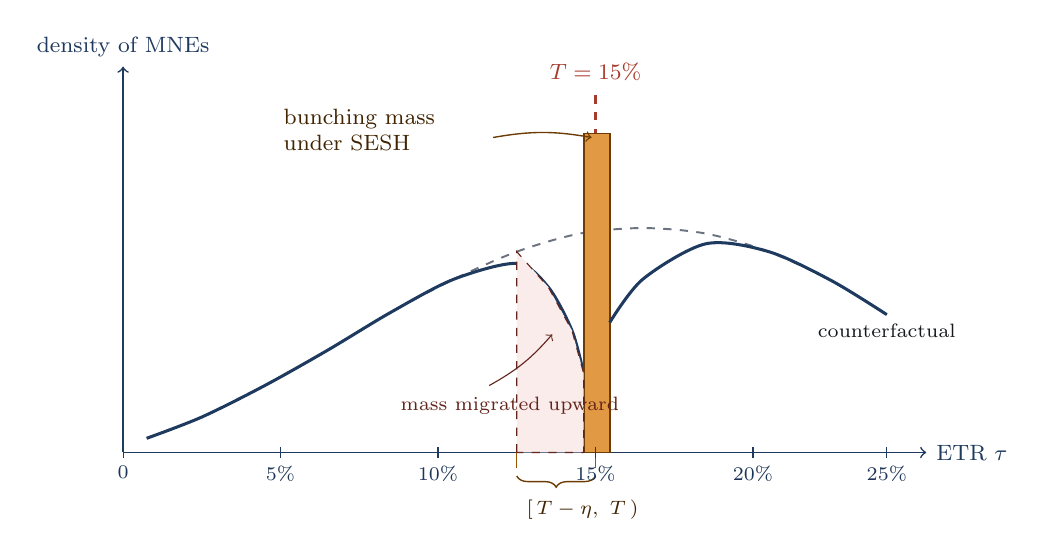
\begin{tikzpicture}[font=\small]
  % Coordinate system
  \def\xmax{10.0}
  \def\ymax{4.6}

  % Axes
  \draw[->, thesisNavy, line width=0.6pt] (0,0) -- (\xmax+0.2, 0) node[right, font=\footnotesize] {ETR $\tau$};
  \draw[->, thesisNavy, line width=0.6pt] (0,0) -- (0, \ymax+0.3) node[above, font=\footnotesize] {density of MNEs};

  % x-tick: 15%
  \def\Tx{6.0}
  \draw[thesisRed!85!black, dashed, line width=0.9pt] (\Tx,0) -- (\Tx,\ymax);
  \node[font=\footnotesize, thesisRed!85!black, anchor=south] at (\Tx,\ymax) {$T = 15\%$};

  % Counterfactual smooth density (no policy)
  % Bell-ish, peaked around tau=18
  \draw[thesisGrey, dashed, line width=0.7pt]
    plot[smooth] coordinates {
      (0.3,0.18) (1.0,0.45) (1.8,0.85) (2.6,1.30) (3.4,1.78)
      (4.2,2.20) (5.0,2.55) (5.8,2.78) (6.6,2.85) (7.4,2.78)
      (8.2,2.55) (9.0,2.18) (9.7,1.75)};
  \node[font=\scriptsize, thesisGrey!20!black, anchor=west] at (8.7, 1.55) {counterfactual};

  % Post-policy density: dip just before T, spike at T
  \draw[thesisNavy, line width=1.1pt]
    plot[smooth] coordinates {
      (0.3,0.18) (1.0,0.45) (1.8,0.85) (2.6,1.30) (3.4,1.78)
      (4.2,2.20) (5.0,2.40) (5.4,2.10) (5.7,1.55) (5.85,1.0)};

  % Spike (bunching mass) at 15%
  \fill[thesisOrange!75, draw=thesisOrange!50!black, line width=0.6pt]
    (5.85,0) rectangle (6.18, 4.05);
  \draw[thesisOrange!50!black, ->, line width=0.5pt] (4.7, 4.0) to[bend left=10] (5.95, 4.0);
  \node[font=\footnotesize, thesisOrange!30!black, align=left] at (3.0, 4.1)
    {bunching mass\\under SESH};

  % Resume after T
  \draw[thesisNavy, line width=1.1pt]
    plot[smooth] coordinates {
      (6.18,1.65) (6.6,2.20) (7.4,2.65) (8.2,2.55) (9.0,2.18) (9.7,1.75)};

  % Bunching window [T-eta, T)
  \def\TminEta{5.0} % Left boundary aligned with dashed reference line
  \draw[thesisOrange!70!black, line width=0.5pt] (\TminEta,0.05) -- (\TminEta,-0.20);
  \draw[thesisOrange!70!black, line width=0.5pt] (\Tx,0.05) -- (\Tx,-0.20);
  \draw[decorate, decoration={brace, mirror, amplitude=4pt}, thesisOrange!50!black, line width=0.5pt]
    (\TminEta,-0.30) -- (\Tx,-0.30);
  \node[font=\scriptsize, thesisOrange!30!black, anchor=north west]
    at (\TminEta, -0.48) {$[\,T-\eta,\ T\,)$};

  % x ticks
  \foreach \xv/\lbl in {0/0, 2/{5\%}, 4/{10\%}, 6/{15\%}, 8/{20\%}, 9.7/{25\%}}{
    \draw[thesisNavy] (\xv, 0.07) -- (\xv, -0.07);
    \node[below, font=\scriptsize, thesisNavy!90!black] at (\xv, -0.05) {\lbl};
  }

  % Mass missing region (hatched)
  \fill[thesisRed!10, draw=thesisRed!50!black, dashed, line width=0.4pt]
    (5.0, 0) -- (5.0, 2.55) -- (5.4,2.10) -- (5.7,1.55) -- (5.85,1.0) -- (5.85,0) -- cycle;
  \node[font=\scriptsize, thesisRed!50!black, anchor=west] at (3.4, 0.6) {mass migrated upward};
  \draw[thesisRed!50!black, ->, line width=0.4pt] (4.65, 0.85) to[bend right=10] (5.45, 1.5);
\end{tikzpicture}
\caption[Bunching at the 15\% threshold under the Simplified ETR Safe Harbour.]{Density of jurisdiction-level ETRs before and after the introduction of the Simplified ETR Safe Harbour. The dashed grey curve represents the counterfactual density absent any policy response, the solid navy curve represents the post-policy density. MNEs whose pre-policy ETR lies in the band $[T-\eta,\ T)$ migrate upward, producing the orange spike at the 15\% threshold. This is the \emph{notch} response that the SESH creates: the cost of falling just below 15\% is disproportionate to the saving, since the alternative is the full GloBE computation. The methodology models this band by setting $\beta_{j,t}=0$ for jurisdictions with $\tau_{j,t}\in[T-\eta,T)$.}
\label{fig:sesh_bunching}
\end{figure}

The pipeline incorporates this response through a two-regime rule applied to \eqref{eq:beta_aggregated}:
\begin{equation}\label{eq:regime}
\hat{\beta}_{j,t}^{\text{applied}} = \begin{cases}
0 & \text{if } \tau_{j,t} \in [T - \eta,\; T), \\[2pt]
\hat{\beta}_{j,t} & \text{if } \tau_{j,t} < T - \eta,
\end{cases}
\end{equation}
with $T = 0.15$ and a baseline bandwidth of $\eta = 0.02$. Inside the bunching band $[T-\eta, T)$, jurisdictions reach the safe harbour through covered-tax and income management alone; the top-up tax is set to zero and pre-tax profit stays in place. Below the band, the gap cannot be closed through accounting adjustments and the semi-elasticity response of \eqref{eq:beta_aggregated} applies. The bandwidth $\eta$ is a sensitivity parameter: $\eta \in \{0.01, 0.03\}$ bracket conservative and expansive variants, with the $\eta = 0.02$ baseline anchored on the dispersion evidence of \citet{hugger2026} and on the plausible cumulative scope of documented GloBE accounting adjustments.\footnote{The rule is a sharp upper bound on bunching behaviour: it assumes that \emph{every} jurisdiction inside $[T-\eta,T)$ reaches the safe harbour, whereas in reality the bunching mass depends on the distribution of ETRs within the band and on the within-jurisdiction elasticity of the simplified ETR with respect to covered-tax choices. A structural notch-bunching estimation would require firm-level data that public CbCR does not provide, and is beyond the scope of this thesis.}

\subsubsection{Redistribution of reallocated profit}\label{sec:reallocation}

Equation \eqref{eq:beta_aggregated} removes profit from the low-tax affiliate; it does not say where that profit is re-reported. Johannesen's model predicts return to the non-haven source jurisdictions that host the underlying real activity, but CbCR data cannot trace individual shifted euros. The thesis therefore adopts the formulary reallocation of \citet{garcia-bernardo2024}:
\begin{equation}\label{eq:reallocation}
R_i = \tfrac{1}{4}\frac{N_i}{\sum_{k} N_k} + \tfrac{1}{4}\frac{W_i}{\sum_{k} W_k} + \tfrac{1}{2}\frac{\text{UPR}_i}{\sum_{k} \text{UPR}_k},
\end{equation}
with $N_i$ employment, $W_i$ payroll, and $\text{UPR}_i$ unrelated-party revenue of MNE activity in destination $i$. Summation is restricted to destinations with $\tau_{i,t} \geq T$ so that reallocated profit is not mechanically re-deposited in a second haven.

Redistribution does not itself generate EU revenue. An additional euro sent to a jurisdiction with $\tau_{i,t}\ge T$ enters its GloBE base above the floor and contributes zero to the top-up; EU revenue from the GMT is determined entirely by the low-taxed source, not by the high-tax destination. The step is therefore diagnostic: \eqref{eq:reallocation} verifies profit conservation across counterfactuals and checks whether the implied re-reporting pattern aligns with the distribution of real activity. The SBIE is evaluated on \emph{pre-response} payroll and tangible assets throughout, holding the substance shield fixed across counterfactual simulations. Allowing substance to move in the same period would conflate two conceptually distinct margins: the short-run profit-allocation response identified by the semi-elasticity, and the long-run real-activity response documented in \citet{bilicka2022} and \citet{suarezserrato2018} and discussed in Section \ref{sec:benchmarks_unmodelled}.

\subsubsection{Uncertainty quantification}\label{sec:beta_uncertainty}

The reallocation factor $\hat{\beta}_{j,t}$ is a nonlinear transformation of two estimated coefficients and one specification choice. Three uncertainty channels enter it: sampling error in the coefficients, functional-form uncertainty, and extrapolation uncertainty below the observed ETR support. Each is reported separately so that the dominant source of spread in the revenue estimate is transparent.

\emph{Sampling uncertainty.} A pairs cluster bootstrap draws 1{,}000 replicate samples of affiliate jurisdictions with replacement from the estimation panel. Each replicate re-estimates the semi-elasticity coefficients, recomputes the closed-form counterfactual in \eqref{eq:cf_linear}--\eqref{eq:cf_log}, applies the safe-harbour regime \eqref{eq:regime}, and runs the full revenue pipeline. The 2.5th and 97.5th percentiles of the replicate distribution form the reported confidence intervals. A delta-method approximation is computed in parallel as a check: the gradient of $R(\hat{\beta})$ with respect to $(\hat{\beta}_3, \hat{\beta}_4)$ is evaluated at the point estimates and the asymptotic variance is $\nabla R^{\prime}\, \hat{V}\, \nabla R$, with $\hat{V}$ the cluster-robust variance matrix from Section \ref{sec:estimation}.

\emph{Functional-form uncertainty.} The BIC and Vuong test identify a preferred specification, but preference is not uniqueness. All three specifications are reported side by side for every scenario, and the spread across forms is labelled the functional-form range. In the factorial design of Section \ref{sec:factorial}, functional form is kept as its own dimension, so its contribution to the revenue range is isolated from cluster-bootstrap variation.

\emph{Extrapolation uncertainty.} The quadratic and logarithmic specifications predict semi-elasticities that rise sharply below the lowest ETR observed in the estimation sample. A \emph{no-extrapolation} variant caps $\hat{\varepsilon}(\tau)$ at $\hat{\varepsilon}(\tau_{\min})$ for all $\tau < \tau_{\min}$, where $\tau_{\min}$ is the 5th percentile of observed affiliate-level ETRs. The gap between the main and no-extrapolation estimates quantifies the dependence of the headline revenue number on out-of-sample functional-form assumptions.

\subsection{Revenue allocation and the Side-by-Side Safe Harbour}\label{sec:sbs}\label{sec:jan2026}

Once the pre-allocation top-up liability is computed, a policy regime determines which jurisdiction collects it. Under the standard GloBE rule order, the source jurisdiction collects the top-up tax via a QDMTT; if no QDMTT is in place, the parent jurisdiction collects via the IIR. If the parent has not implemented the IIR either, third-country jurisdictions collect via the UTPR.

The January 2026 Side-by-Side (SbS) Safe Harbour disrupts this rule order \citep{oecd2026}. MNE groups headquartered in jurisdictions with a ``Qualified SbS Regime'' may elect a deemed top-up tax of zero under both the IIR and the UTPR for all their operations. The United States is currently the only jurisdiction with a qualified regime.\footnote{The SbS Safe Harbour requires both an eligible domestic tax regime \emph{and} an eligible worldwide tax regime. The US qualifies through its combination of the corporate income tax (domestic) and the GILTI regime (worldwide). See \citet{oecd2026}, Chapter 1, Section 4.} US-parented MNEs are therefore exempt from IIR and UTPR enforcement.

QDMTTs remain entirely unaffected by the SbS Safe Harbour. Jurisdictions that implement a QDMTT retain the right to tax US-owned affiliates operating within their borders, regardless of the SbS election. The SbS package therefore creates a sharp discontinuity: for US-parented MNEs, the IIR and UTPR channels are switched off, but the QDMTT channel remains operational. 

Revenue under the SbS regime:
\begin{align}
R_{j,t}^{\text{QDMTT}} &= \sum_p \text{TopUp}_{p,j,t} \times \mathbb{1}_j^{\text{Q}} \label{eq:qdmtt_sbs} \\
R_{p,t}^{\text{IIR}} &= \sum_j \text{TopUp}_{p,j,t} \times (1 - \mathbb{1}_j^{\text{Q}}) \times (1 - \mathbb{1}_p^{\text{SbS}}) \label{eq:iir_sbs} \\
R_{j,t}^{\text{UTPR}} &= \sum_p \text{TopUp}_{p,j,t} \times (1 - \mathbb{1}_j^{\text{Q}}) \times \mathbb{1}_p^{\text{SbS}} \times 0 = 0 \label{eq:utpr_sbs}
\end{align}

Equation \eqref{eq:utpr_sbs} formalises the core consequence: UTPR revenue from US-parented groups is mechanically zero.

\begin{figure}[H]
\centering
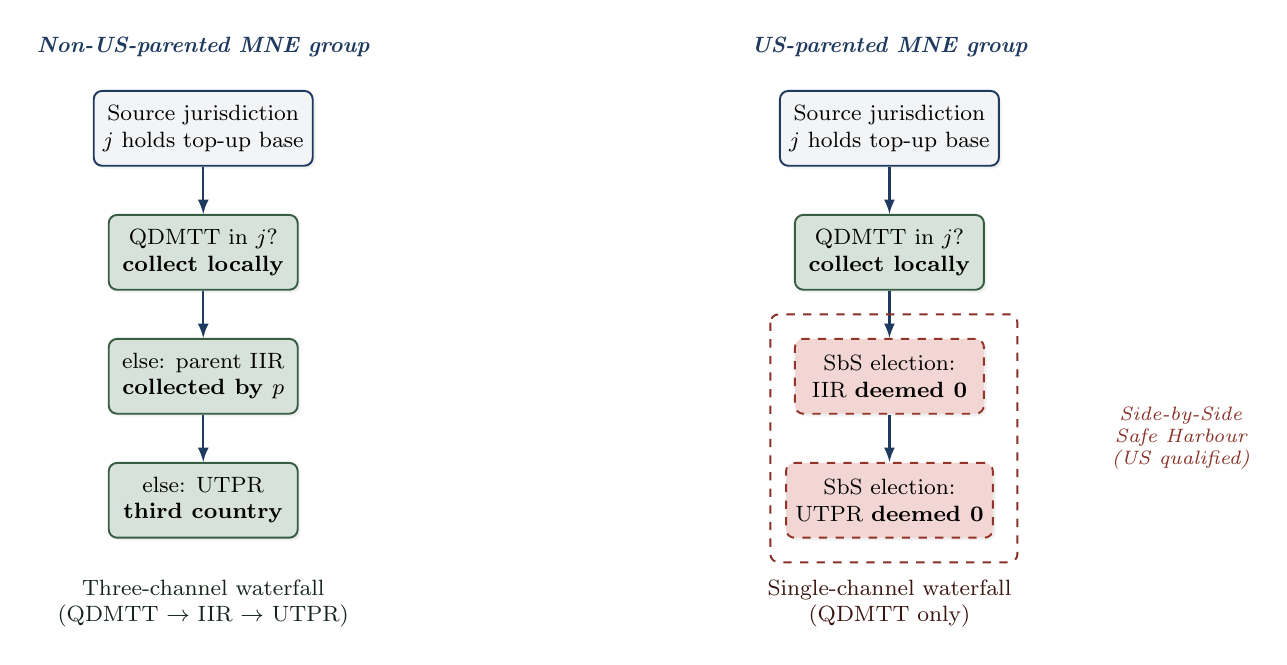
\begin{tikzpicture}[font=\small, node distance=0.6cm,
    rule/.style={draw=thesisNavy, line width=0.7pt, rounded corners=3pt,
                 fill=thesisLight, minimum width=2.4cm, minimum height=0.95cm,
                 align=center, font=\footnotesize,
                 drop shadow={shadow xshift=1pt, shadow yshift=-1pt, opacity=0.12}},
    on/.style={fill=thesisGreen!22, draw=thesisGreen!75!black},
    off/.style={fill=thesisRed!22, draw=thesisRed!75!black, dashed}]

  % Header rows
  \node[font=\footnotesize\itshape, thesisNavy] (h1) {\textbf{Non-US-parented MNE group}};
  \node[font=\footnotesize\itshape, thesisNavy, right=4.6cm of h1] (h2) {\textbf{US-parented MNE group}};

  %  Left column 
  \node[rule, below=0.3cm of h1] (sl) {Source jurisdiction\\$j$ holds top-up base};
  \node[rule, on, below=of sl] (q1) {QDMTT in $j$?\\\textbf{collect locally}};
  \node[rule, on, below=of q1] (i1) {else: parent IIR\\\textbf{collected by $p$}};
  \node[rule, on, below=of i1] (u1) {else: UTPR\\\textbf{third country}};

  %  Right column 
  \node[rule, below=0.3cm of h2] (sr) {Source jurisdiction\\$j$ holds top-up base};
  \node[rule, on, below=of sr] (q2) {QDMTT in $j$?\\\textbf{collect locally}};
  \node[rule, off, below=of q2] (i2) {SbS election:\\IIR \textbf{deemed 0}};
  \node[rule, off, below=of i2] (u2) {SbS election:\\UTPR \textbf{deemed 0}};

  % Arrows
  \foreach \a/\b in {sl/q1, q1/i1, i1/u1} \draw[thesis arrow] (\a) -- (\b);
  \foreach \a/\b in {sr/q2, q2/i2, i2/u2} \draw[thesis arrow] (\a) -- (\b);

  % SbS exemption banner spanning right column
  \draw[thesisRed!70!black, line width=0.7pt, rounded corners=3pt, dashed]
    ([xshift=-0.3cm, yshift=0.3cm]i2.north west) rectangle ([xshift=0.3cm, yshift=-0.3cm]u2.south east);
  \node[font=\scriptsize\itshape, thesisRed!70!black, align=center]
    at ($(i2)!0.5!(u2) + (3.7, 0)$) {Side-by-Side\\Safe Harbour\\(US qualified)};

  % Outcome at the bottom of each column
  \node[below=0.4cm of u1, font=\footnotesize, thesisGreen!30!black, align=center]
    {Three-channel waterfall\\(QDMTT $\to$ IIR $\to$ UTPR)};
  \node[below=0.4cm of u2, font=\footnotesize, thesisRed!30!black, align=center]
    {Single-channel waterfall\\(QDMTT only)};

\end{tikzpicture}
\caption[Allocation rule under the Side-by-Side Safe Harbour.]{Collection waterfall under the original GloBE rule order versus the January 2026 Side-by-Side Safe Harbour. For non-US-parented MNE groups, the QDMTT/IIR/UTPR cascade is unaffected. For US-parented groups, an SbS election sets both IIR and UTPR top-up to zero, leaving QDMTTs as the only operative collection channel. EU Member States that have not implemented a QDMTT therefore lose the entire top-up tax claim against US-owned affiliates, formalised in equation \eqref{eq:utpr_sbs}.}
\label{fig:sbs_waterfall}
\end{figure}

\subsection{The revenue pipeline}\label{sec:pipeline}

The three stages and the allocation rule combine into a single multiplicative framework.\footnote{The revenue pipeline decomposition is original to this thesis. The individual components draw on \citet{hugger2026} (Stage 1), \citet{schjelderup2024} and \citet{devereux2023} (Stage 2), and the panel-estimated semi-elasticities (Section \ref{sec:estimation}) for Stage 3. No prior study combines these into a single multiplicative framework that makes the sources of revenue uncertainty simultaneously visible and exactly decomposable.} For each bilateral parent--affiliate cell, the pre-allocation top-up liability is:
\begin{equation}\label{eq:pipeline}
L_{p,j,t} = \underbrace{\ell_{p,j,t} \cdot \bar{\delta}_{j,t}^{\text{top}}}_{\text{Stage 1: ETR filter}} \times \underbrace{\left(1 - \bar{\phi}_{p,j,t}\right)}_{\text{Stage 2: SBIE filter}} \times \underbrace{\left(1 - \beta_{j,t}\right)}_{\text{Stage 3: behavioural filter}}
\end{equation}
where $\ell_{p,j,t} = s_{j,t}^{<T} \cdot \pi_{p,j,t}^{*}$ is low-taxed profit (Section \ref{sec:etr_measurement}), $\bar{\delta}_{j,t}^{\text{top}}$ is the average top-up rate on that low-taxed portion, $\bar{\phi}_{p,j,t}$ is the SBIE shield (Section \ref{sec:SBIE}), and $\beta_{j,t}$ is the behavioural reallocation fraction (Section \ref{sec:behavioural}). The allocation rule then distributes the liability:
\begin{equation}\label{eq:allocation}
R_{s,t}^{(r)} = \sum_p \sum_j a_{s,p,j,t}^{(r)} \cdot L_{p,j,t}
\end{equation}
where $a_{s,p,j,t}^{(r)}$ is the regime-specific allocation weight implied by the QDMTT/IIR/UTPR rule order under policy regime $r$ (Section \ref{sec:sbs}).

Revenue uncertainty compounds across stages. A positive Stage 1 $\times$ Stage 2 interaction indicates that the distributional approach reveals low-taxed profit concentrated in capital-intensive sectors with high $\phi$, so the expanded base is partially offset by stronger SBIE shielding. The pipeline structure identifies which data improvements would most reduce uncertainty: if Stage 1 dominates variation, within-jurisdiction ETR data are the priority; if Stage 2 dominates, better CbCR coverage of tangible assets and payroll matters more.

\subsection{Counterfactual decomposition}\label{sec:decomposition}

\subsubsection{Factor definitions}\label{sec:factors}

Five binary factors drive the variation in GMT revenue estimates. Table \ref{tab:factors} defines each factor and its two levels.

\begin{table}[H]
\centering
\caption{Decomposition factors}
\label{tab:factors}
\small
\begin{tabular}{@{}clp{3.5cm}p{3.5cm}@{}}
\toprule
Factor & Name & Baseline ($x_i = 0$) & Alternative ($x_i = 1$) \\
\midrule
1 & ETR measurement & Jurisdiction-average & Within-jurisdiction percentile approximation (Hugger-style) \\
2 & Substance specification & Aggregate SBIE & Sectoral SBIE with SBTI-capacity overlay ($\kappa$) \\
3 & SBIE carve-out rates & Initial (10\%/8\%) & Long-run (5\%/5\%) \\
4 & SbS carve-out & Universal IIR/UTPR & SbS Safe Harbour (US exempt from IIR/UTPR) \\
5 & Behavioural response & None (mechanical) & Panel-estimated nonlinear semi-elasticities + safe-harbour bunching \\
\bottomrule
\end{tabular}
\end{table}

Each factor maps to a pipeline stage. Factor 1 switches $s_j^{<T}$ between binary and continuous. Factor 2 changes $\bar{\phi}_{p,j,t}$ from the aggregate CbCR value to the sectoral FATS-based estimate with the SBTI-capacity overlay ($\kappa_{j,s,t}$ from equation \ref{eq:sbti_capacity}). Factor 3 moves from initial to long-run carve-out rates. Factor 4 switches the allocation weight $a_{s,p,j,t}^{(r)}$ between universal and SbS regimes. Under the alternative, IIR and UTPR top-up variables are set to zero for all observations where the parent jurisdiction is the United States (equations \ref{eq:iir_sbs}--\ref{eq:utpr_sbs}); QDMTTs remain fully operational in both scenarios. Factor 5 introduces $\hat{\beta}_j > 0$ via the panel-estimated nonlinear semi-elasticities (equation \ref{eq:beta_estimated}) and sets $\hat{\beta}_j = 0$ for jurisdictions in the bunching band $[T - \eta, T)$.

\subsubsection{Factorial design}\label{sec:factorial}

Revenue is computed under all $2^5 = 32$ factor combinations.\footnote{The application of a full factorial design to GMT revenue estimation is original to this thesis. \citet{barake2022} and \citet{hugger2026} vary parameters one at a time; neither presents a design that makes all factor interactions simultaneously visible and exactly decomposable via an ANOVA identity.} Let $\mathbf{x} = (x_1, \ldots, x_5) \in \{0, 1\}^5$ denote a configuration. The revenue under configuration $\mathbf{x}$ for EU Member State $j$ in year $t$ is $R_{j,t}(\mathbf{x})$.

\subsubsection{Variance decomposition}\label{sec:anova}

The $2^5$ factorial design permits an exact additive decomposition of the total sum of squares of revenue estimates into main effects, two-way interactions, and higher-order interactions. The ANOVA identity for a balanced $2^K$ design with $K = 5$ factors decomposes the total variation of $R(\mathbf{x})$ across the 32 configurations as:
\begin{equation}\label{eq:anova}
\text{SS}_{\text{total}} = \sum_{i=1}^{5} \text{SS}_i + \sum_{i<k} \text{SS}_{ik} + \sum_{i<k<l} \text{SS}_{ikl} + \cdots + \text{SS}_{12345}
\end{equation}
where $\text{SS}_i$ is the sum of squares attributable to the main effect of factor $i$, $\text{SS}_{ik}$ is the sum of squares attributable to the two-way interaction between factors $i$ and $k$, and so forth. With five binary factors, the decomposition yields 5 main effects, 10 two-way interactions, 10 three-way interactions, 5 four-way interactions, and 1 five-way interaction, totalling $2^5 - 1 = 31$ orthogonal contrasts that exactly exhaust the total variation.

Each effect is computed as the squared contrast divided by the number of observations. For a main effect of factor $i$:
\begin{equation}\label{eq:main_effect}
\text{SS}_i = \frac{n}{4} \left(\bar{R}_{x_i = 1} - \bar{R}_{x_i = 0}\right)^2
\end{equation}
where $\bar{R}_{x_i = 1}$ and $\bar{R}_{x_i = 0}$ are the mean revenues across all configurations where factor $i$ is at its high and low levels respectively, and $n = 32$ is the total number of configurations. For a two-way interaction:
\begin{equation}\label{eq:interaction_effect}
\text{SS}_{ik} = \frac{n}{4} \left(\bar{R}_{x_i = 1, x_k = 1} - \bar{R}_{x_i = 1, x_k = 0} - \bar{R}_{x_i = 0, x_k = 1} + \bar{R}_{x_i = 0, x_k = 0}\right)^2
\end{equation}
A non-zero two-way interaction $\text{SS}_{ik}$ indicates that the effect of factor $i$ on revenue depends on the level of factor $k$. For instance, a positive $\text{SS}_{15}$ (ETR measurement $\times$ behavioural response) would indicate that the distributional ETR approach reveals low-taxed profit concentrated at very low pre-reform ETRs, where the nonlinear behavioural response is strongest, thereby amplifying the revenue difference between the two ETR approaches.

The share of explained variance attributable to each effect is $\eta_i^2 = \text{SS}_i / \text{SS}_{\text{total}}$. The decomposition is performed at three levels: pooled across all 27 EU Member States and years, identifying which factors drive aggregate EU revenue variation, separately for each EU Member State (pooling across years), identifying country-specific dominant factors, and for selected EU Member States of policy interest (the Netherlands, Ireland, Luxembourg, Germany, France).

\subsubsection{Scenario spread versus estimation uncertainty}\label{sec:two_uncertainties}

The factorial design separates two conceptually distinct sources of uncertainty in GMT revenue estimates. \emph{Scenario spread} is the range of revenue estimates across the 32 modelling configurations for a given country--year cell, holding the semi-elasticity coefficients at their point estimates. This spread is driven by modelling assumptions that cannot be estimated from the data: the choice between average and distributional ETR measurement, whether to use aggregate or sectoral SBIE, and whether the SbS regime applies. \emph{Estimation uncertainty} is the width of the bootstrapped 90\% confidence interval around the revenue estimate within a single scenario, driven by the statistical precision of the semi-elasticity coefficients.

For each EU Member State $j$ and year $t$, the ratio of scenario spread to estimation uncertainty is:
\begin{equation}\label{eq:spread_ratio}
\Lambda_{j,t} = \frac{\max_{\mathbf{x}} R_{j,t}(\mathbf{x}) - \min_{\mathbf{x}} R_{j,t}(\mathbf{x})}{q_{0.95}(R_{j,t}^{*}) - q_{0.05}(R_{j,t}^{*})}
\end{equation}
where $R_{j,t}^{*}$ denotes the preferred-scenario revenue estimate across bootstrap replications. A ratio $\Lambda > 1$ indicates that the modelling assumptions matter more than the statistical precision of the semi-elasticity estimates. In that case, the debate about \emph{how} to estimate GMT revenue dominates the question of \emph{how precisely} the key behavioural parameter is known. This distinction is directly policy-relevant. If $\Lambda \gg 1$, reducing revenue uncertainty requires better data or institutional knowledge (such as within-jurisdiction ETR microdata), not more observations for the semi-elasticity regression.

\subsection{Hypotheses}\label{sec:hypotheses}

The hypotheses below are derived from the literature reviewed in Section \ref{sec:literature} and from the structure of the revenue pipeline. Each hypothesis states the a-priori expectation, the null hypothesis against which it is tested, and the test procedure. The five hypotheses map to the three subquestions: H1 addresses SQ1 (semi-elasticity estimation), H2 and H3 address SQ2 (factorial decomposition), and H4 and H5 address SQ3 (January 2026 provisions).

\textbf{H1: The profit-shifting semi-elasticity is nonlinear across the ETR distribution, rising sharply at low ETRs, and the logarithmic functional form captures this nonlinearity better than the linear or quadratic alternatives.}

\textit{Null hypothesis.} $H_0$: The semi-elasticity of reported profits with respect to the ETR is constant across the tax rate distribution ($\beta_4 = 0$ in both the quadratic and logarithmic specifications), and the linear model fits the CbCR panel at least as well as the nonlinear alternatives.

\textit{A-priori expectation.} Profit shifting via intellectual property relocation and intra-group lending involves largely fixed set-up costs (legal structures, treaty planning, intercompany agreements). As the ETR approaches zero, these fixed costs become a smaller fraction of the tax saving, so the marginal MNE finds it profitable to shift at increasingly small tax differentials. This produces a convex cost function and a semi-elasticity that rises sharply at low ETRs. \citet{dowd2017} document this on US IRS data: the semi-elasticity at a 5\% statutory rate is 4.7, compared to 0.7 at 30\%. \citet{garcia-bernardo2024} confirm the pattern on a 2017 OECD CbCR cross-section, finding that the logarithmic specification (which allows unbounded semi-elasticity as $\tau \to 0$) dominates the quadratic (which imposes a turning point). I expect the logarithmic specification to produce the lowest BIC and to be preferred by the Vuong test, and I expect the panel-estimated semi-elasticity at $\tau = 0.05$ to exceed the meta-regression consensus of 0.8 \citep{heckemeyer2017} by a factor of at least three. The panel structure adds within-pair variation that the cross-section lacks, reducing omitted-variable bias from time-invariant bilateral confounders.

\textit{Test.} The three specifications (equations \ref{eq:panel_linear}, \ref{eq:panel_quadratic}, \ref{eq:panel_log}) are estimated on the same sample. First, the BIC ranks all three; the BIC penalises complexity more heavily than the AIC and is appropriate because the models differ in the number of tax coefficients. Second, the \citet{vuong1989} test compares the quadratic and logarithmic specifications, which are non-nested. The Davidson--MacKinnon $J$-test and the Clarke (2007) sign test serve as robustness checks.\footnote{The Vuong test compares observation-level log-likelihoods of two non-nested models. It tests $H_0$: both models are equally close to the true data-generating process. A significant positive statistic favours one model over the other.} H1 is supported if the logarithmic specification has the lowest BIC, the Vuong test rejects the quadratic in favour of the logarithmic at $p < 0.05$, and $\hat{\varepsilon}(0.05) > 0.8$. H1 is rejected if the linear specification is preferred, or if the panel-estimated semi-elasticities at low ETRs are comparable to the meta-regression consensus. That would imply that the nonlinearity observed in the cross-section is an artefact of omitted bilateral heterogeneity absorbed by the pair fixed effects.

\textbf{H2: The ETR measurement method accounts for the largest share of explained variance in the factorial decomposition of GMT revenue estimates.}

\textit{Null hypothesis.} $H_0$: The five main effects contribute equally to the total variance of revenue estimates across the 32 factorial configurations ($\eta_1^2 = \eta_k^2$ for all $k$).

\textit{A-priori expectation.} The ETR measurement factor (jurisdiction-average vs.\ distributional) operates at the base level of the revenue pipeline: it determines $s_{j,t}^{<T}$, the share of profit classified as low-taxed, on which all subsequent stages act multiplicatively. \citet{hugger2026} show that 53.2\% of global low-taxed profit lies in jurisdictions with average ETRs above 15\%, implying that the distributional approach approximately doubles the measured GMT base. This base-level doubling is expected to dominate the multiplicative adjustments from the other four factors. The SBIE shields 57\% of GloBE income on average \citep{devereux2023}, so switching from aggregate to sectoral SBIE changes revenue by the difference in $\phi$ across specifications. This is a second-order effect relative to doubling the base. The behavioural response under the linear benchmark implies an 8\% profit reduction at $\tau = 5\%$; even the nonlinear logarithmic response, applied to a fixed base, generates less variation than switching between a base of $X$ and $2X$. A potential rejection arises if the panel-estimated nonlinear semi-elasticities produce behavioural adjustments large enough to rival the base doubling, which would occur if the EU low-tax base is concentrated at near-zero pre-reform ETRs where the logarithmic semi-elasticity is steepest.

\textit{Test.} In the ANOVA decomposition of the $32 \times 27 \times T$ revenue matrix (32 scenarios, 27 EU Member States, up to 7 fiscal years), the share of total sum of squares attributable to each main effect ($\eta_i^2 = \text{SS}_i / \text{SS}_{\text{total}}$) is compared. H2 is supported if $\eta_1^2 > \eta_k^2$ for all $k \in \{2, 3, 4, 5\}$.

\textbf{H3: Factor interactions account for an economically significant share of total revenue variation, implying that one-at-a-time sensitivity analysis understates the true uncertainty range.}

\textit{Null hypothesis.} $H_0$: All interaction effects are zero; the total variation is fully explained by the five main effects ($\text{SS}_{\text{interactions}} = 0$).

\textit{A-priori expectation.} Published GMT revenue estimates vary parameters individually: \citet{barake2022} report estimates with and without behavioural responses; \citet{hugger2026} compare average and distributional ETR approaches; \citet{boukal2026} decompose by collection channel. None examines joint variation. The revenue pipeline (equation \ref{eq:pipeline}) is multiplicative, which makes non-zero interactions likely. The behavioural response reduces a \emph{percentage} of the base, so its absolute effect depends on whether the base was measured with the average or distributional approach (the Factor 1 $\times$ Factor 5 interaction). Similarly, the SBIE filter interacts with ETR measurement if the newly revealed low-taxed profit (from the distributional approach) is concentrated in holding/IP entities with low substance, differing from the composition of profit already classified as low-taxed under the average approach. The SbS carve-out (Factor 4) interacts with ETR measurement (Factor 1) if the distributional approach reveals substantial US-parented low-taxed profit in non-QDMTT jurisdictions. I expect the total interaction share to exceed 10\%.

\textit{Test.} The share of total sum of squares attributable to all interaction terms (two-way through five-way) is computed: $\eta_{\text{int}}^2 = \sum \text{SS}_{\text{interactions}} / \text{SS}_{\text{total}}$. H3 is supported if $\eta_{\text{int}}^2 \geq 0.10$. The 10\% threshold is economically motivated: for the Netherlands, whose projected GMT revenue is \EUR466 million \citep{36369_3}, a 10\% interaction share implies that one-at-a-time analysis misses roughly \EUR47 million in revenue variation. The interaction terms are jointly tested with an $F$-test. The ratio $\Lambda_{j,t}$ (equation \ref{eq:spread_ratio}) is reported for each EU Member State; $\Lambda > 1$ indicates that modelling assumptions dominate statistical estimation uncertainty.

\textbf{H4: The SbS Safe Harbour reduces aggregate EU GMT revenue collected through the IIR and UTPR channels, with the revenue loss concentrated in Member States that have not implemented a QDMTT.}

\textit{Null hypothesis.} $H_0$: The SbS Safe Harbour has no effect on aggregate EU GMT revenue ($\bar{R}^{\text{SbS}} = \bar{R}^{\text{universal}}$), and the revenue change does not vary with QDMTT implementation status.

\textit{A-priori expectation.} The SbS mechanically eliminates IIR and UTPR collection on US-parented MNE groups (equations \ref{eq:qdmtt_sbs}--\ref{eq:utpr_sbs}). QDMTTs remain fully operational. The net effect on a Member State's revenue therefore depends on two quantities: the share of its low-taxed profit attributable to US-parented MNEs, and whether it has implemented a QDMTT. Member States with a QDMTT retain the right to tax US-owned affiliates domestically. Those without one lose the UTPR channel entirely. US-parented MNEs account for approximately 30--40\% of global CbCR profits; the Dutch government projected a \EUR120 million annual reduction from the SbS package \citep{1028}. I expect aggregate EU revenue to decline significantly, with the decline concentrated in Member States without a QDMTT.

\textit{Test.} Revenue under Factor 4 = 0 (universal IIR/UTPR) is compared with revenue under Factor 4 = 1 (SbS) across all 16 combinations of the other four factors, pooled across 27 EU Member States and fiscal years. A Wilcoxon signed-rank test assesses whether the paired difference is significantly negative; the non-parametric test is appropriate because the revenue differences are unlikely to be normally distributed given the skewed profit distribution. The distributional prediction is tested by regressing the country-level average revenue change ($\overline{\Delta R}_j$) on a QDMTT implementation indicator, controlling for the US-parented profit share. H4 is supported if the aggregate paired difference is significantly negative ($p < 0.05$) and the QDMTT coefficient is significantly positive (Member States with a QDMTT lose less revenue).

\textbf{H5: The SBTI Safe Harbour reduces the effective tax floor heterogeneously across EU sectors, with the reduction largest in capital-intensive sectors.}

\textit{Null hypothesis.} $H_0$: The SBTI-induced reduction in the effective tax floor is uniform across sectors ($\partial \Delta\tau^{\text{floor}} / \partial (A/\pi) = 0$).

\textit{A-priori expectation.} The SBTI allows MNEs to treat qualifying tax incentives as additions to covered taxes, bounded by a Substance Cap tied to payroll and tangible assets (equation \ref{eq:substance_cap}). Capital-intensive sectors benefit doubly: larger SBIE carve-outs \emph{and} higher Substance Caps. \citet{schjelderup2024} predict that the SBIE functions as a \emph{de facto} production subsidy favouring capital-intensive industries; the SBTI amplifies this by adding a second substance-linked benefit. Asset-light sectors (financial services, IP licensing) have Substance Caps approaching zero and therefore cannot utilise the SBTI. \citet{devereux2023} find SBIE-to-profit ratios ranging from below 30\% (financial services) to above 70\% (manufacturing), confirming the sectoral gradient. The countervailing force is that capital-intensive sectors may already face pre-reform ETRs above 15\%, reducing the set of entities for which the SBTI matters. I expect the capital-intensity effect to dominate, producing a negative coefficient: higher $A/\pi$ is associated with a larger reduction (more negative $\Delta\tau^{\text{floor}}$).

\textit{Test.} For each EU Member State $j$ and NACE sector $s$, the change in the effective tax floor when the SBTI overlay is applied ($\Delta \tau_{j,s}^{\text{floor}} = \tau_{j,s}^{\text{floor, with SBTI}} - \tau_{j,s}^{\text{floor, without SBTI}}$) is regressed on the sectoral capital-intensity proxy ($A_{j,s} / \pi_{j,s}$) from the CbCR--FATS combination, with country fixed effects:
\begin{equation}\label{eq:h5_test}
\Delta \tau_{j,s}^{\text{floor}} = \alpha_j + \delta \cdot \frac{A_{j,s}}{\pi_{j,s}} + \varepsilon_{j,s}
\end{equation}
H5 is supported if $\hat{\delta} < 0$ and significant ($p < 0.05$), indicating that capital-intensive sectors experience a larger reduction in the effective tax floor.

\newpage
\section{Results}\label{sec:results}


\newpage
\section{Discussion and conclusion}\label{sec:discussion}

\subsection{Discussion}\label{sec:discussion_main}


\subsection{Policy implications}\label{sec:implications}

\subsection{Limitations}\label{sec:limitations}



\newpage
\printbibliography[heading=bibintoc]

\newpage
\appendix
\renewcommand{\thesection}{\Alph{section}}
\renewcommand{\thetable}{\Alph{section}.\arabic{table}}
\renewcommand{\thefigure}{\Alph{section}.\arabic{figure}}
\renewcommand{\theequation}{\Alph{section}.\arabic{equation}}
\setcounter{table}{0}
\setcounter{figure}{0}
\setcounter{equation}{0}

\section{Data appendix}\label{app:data}

\subsection{CbCR data}\label{app:CbCR}

The CbCR data are split into six ``Tables''.

Each table shares fifteen columns, documented in Table \ref{tab:columns}.

\begin{table}[H]
\centering
\caption{Column structure common to all six CbCR SDMX files}
\label{tab:columns}
\begin{tabular}{@{}lp{9.5cm}@{}}
\toprule
Column name & Description \\
\midrule
\code{DATAFLOW} & Identifier of the SDMX dataflow and version \\
\code{REF\_AREA} & ISO 3166-1 alpha-3 code of the \emph{reporting (parent) jurisdiction}: the country whose tax authority collected and submitted the CbCR data \\
\code{COUNTERPART\_AREA} & ISO 3166-1 alpha-3 code of the \emph{affiliate jurisdiction}: the country where the constituent entity is resident; \code{\_Z} if not applicable; regional aggregates such as \code{WXD} (world excl.\ domestic), \code{W} (world total), and continent codes also appear \\
\code{FREQ} & Frequency; always \code{A} (annual) \\
\code{MEASURE} & The variable being measured (see Table \ref{tab:measures}) \\
\code{UNIT\_MEASURE} & Unit of the observation (see Table \ref{tab:units}) \\
\code{STATISTICAL\_OPERATION} & Statistical transformation applied, if any (see Table \ref{tab:statops}) \\
\code{AGGREGATION\_TYPE} & Unit of observation and aggregation level (see Table \ref{tab:aggtypes}) \\
\code{PROFIT\_GROUPING} & Panel filter (all MNEs, profit-makers only, all incl.\ loss-makers) \\
\code{EFFECTIVE\_TAX\_RATE} & ETR bracket classification; \code{\_Z} if not disaggregated by ETR \\
\code{MNE\_SIZE} & Revenue-based size class of the MNE group; \code{\_Z} if not disaggregated \\
\code{TIME\_PERIOD} & Fiscal year of the reported data \\
\code{OBS\_VALUE} & The observation value in the unit specified by \code{UNIT\_MEASURE}; monetary values are denominated in USD \\
\code{DECIMALS} & Number of decimal places used to express the value \\
\code{OBS\_STATUS} & \code{A} = actual/normal value; \code{Q} = provisional or preliminary value \\
\bottomrule
\end{tabular}
\end{table}


Table \ref{tab:measures} lists all \code{MEASURE} codes that appear across the six CbCR tables, together with the description of the code and the unit in which they are reported. Not all measures appear in all tables; the column \emph{Tables} indicates where each measure is available.

\begin{longtable}{@{}lp{6cm}lp{2.5cm}@{}}
\caption{MEASURE codes in the OECD CbCR database}\label{tab:measures}\\
\toprule
Code & Description & Unit & Tables \\
\midrule
\endfirsthead
\multicolumn{4}{c}{\textit{Table \ref{tab:measures} continued}}\\
\toprule
Code & Description & Unit & Tables \\
\midrule
\endhead
\midrule
\multicolumn{4}{r}{\textit{Continued on next page}}\\
\endfoot
\bottomrule
\endlastfoot
\multicolumn{4}{l}{\textit{Financial aggregates}}\\
\code{PROFIT} & Profit before income tax. The primary measure of taxable profit used in CbCR; susceptible to profit shifting and earnings management & USD & I--IV, VI \\
\code{PROFIT\_ADJ} & Adjusted profit before tax (corrected for intra-group dividends and equity income to reduce double-counting) & USD & I--IV \\
\code{TAX\_ACCRUED} & Income tax accrued (current year charge); the numerator of the CbCR effective tax rate & USD & I--IV, VI \\
\code{TAX\_PAID}  & Income tax paid on a cash basis; may differ from accrued due to timing of payments & USD & I--IV, VI \\
\code{TOT\_REV}  & Total revenue: the sum of unrelated-party and related-party revenues & USD & I--IV, VI \\
\code{UPR}   & Unrelated-party revenue; excludes intra-group transactions & USD & I--VI \\
\code{RPR}   & Related-party revenue; intra-group revenues between constituent entities & USD & I--IV, VI \\
\code{ASSETS}   & Tangible assets, excluding cash and cash equivalents; the denominator of the substance-based income exclusion (payroll component) & USD & I--VI \\
\code{EARNINGS}  & Total payroll costs (compensation of employees); the second component of the SBIE denominator & USD & I--IV, VI \\
\code{STATED\_CAPITAL}& Stated capital and accumulated retained earnings & USD & I--IV, VI \\
\addlinespace
\multicolumn{4}{l}{\textit{Count variables}}\\
\code{EMPLOYEES}  & Number of employees (full-time equivalent); an alternative substance proxy & Persons & I--VI \\
\code{ENTITIES\_COUNT}& Number of constituent entities reporting in that jurisdiction & Entities & I--IV \\
\code{CBCR\_COUNT} & Number of CbCR filings (MNE groups) contributing to the aggregate & MNE groups & I--IV, VI \\
\code{SUBGROUPS\_COUNT}& Number of MNE subgroups & Subgroups & I--IV, VI \\
\addlinespace
\multicolumn{4}{l}{\textit{Derived tax rate}}\\
\code{ETR}   & Effective tax rate computed as \code{TAX\_ACCRUED} / \code{PROFIT} at the jurisdiction level; expressed as a percentage of profit before tax & \% of PBT & I \\
\addlinespace
\multicolumn{4}{l}{\textit{Business-activity count variables (all in Table I, III, IV, VI)}}\\
\code{ACT\_ADMIN} & Number of constituent entities reporting administrative, management or support services as a business activity & EST & I, III, IV, VI \\
\code{ACT\_DOR}  & Number of constituent entities reporting dormant status as a business activity & EST & I, III, IV, VI \\
\code{ACT\_FIN}  & Number of constituent entities reporting regulated financial services as a business activity & EST & I, III, IV, VI \\
\code{ACT\_HOLDING} & Number of constituent entities reporting holding shares or other equity instruments as a business activity & EST & I, III, IV, VI \\
\code{ACT\_IGF}  & Number of constituent entities reporting internal group finance as a business activity & EST & I, III, IV, VI \\
\code{ACT\_INS}  & Number of constituent entities reporting insurance as a business activity & EST & I, III, IV, VI \\
\code{ACT\_IP}  & Number of constituent entities reporting holding or managing intellectual property as a business activity & EST & I, III, IV, VI \\
\code{ACT\_MAN}  & Number of constituent entities reporting manufacturing or production as a business activity & EST & I, III, IV, VI \\
\code{ACT\_OTHER} & Number of constituent entities reporting other business activity & EST & I, III, IV, VI \\
\code{ACT\_PUR}  & Number of constituent entities reporting purchasing or procurement as a business activity & EST & I, III, IV, VI \\
\code{ACT\_RD}  & Number of constituent entities reporting research and development as a business activity & EST & I, III, IV, VI \\
\code{ACT\_SALES} & Number of constituent entities reporting sales, marketing or distribution as a business activity & EST & I, III, IV, VI \\
\code{ACT\_SER}  & Number of constituent entities reporting provision of services to unrelated parties as a business activity & EST & I, III, IV, VI \\
\end{longtable}

The aggregation type defines the unit of observation at which the CbCR data are compiled. 

\begin{table}[H]
\centering
\caption{AGGREGATION\_TYPE codes}
\label{tab:aggtypes}
\begin{tabular}{@{}llp{8cm}@{}}
\toprule
Code & Label & Description \\
\midrule
\code{TOTAL} & Jurisdiction total & Financial variables summed across all MNE groups reporting to the parent jurisdiction's tax authority; the standard aggregate used in \citet{barake2022} \\
\code{TRMNE} & MNE-group level & Variables computed at the level of the individual MNE group and then cross-tabulated by the reporting (parent) jurisdiction; used in Table III to distribute entities across ETR brackets by MNE group \\
\code{TRSUB} & Subsidiary level & Variables computed at the level of the individual constituent entity (subsidiary) and aggregated by its location jurisdiction; used in Table IV to identify where low-taxed profit is booked \\
\code{MNESIZE} & Size class & Variables aggregated within each of five revenue-based size classes of MNE groups; used exclusively in Table VI \\
\bottomrule
\end{tabular}
\end{table}


The ETR brackets are the central dimension of Tables III and IV. Table \ref{tab:etr} documents all codes. 

\begin{table}[H]
\centering
\caption{EFFECTIVE\_TAX\_RATE bracket codes}
\label{tab:etr}
\begin{tabular}{@{}lp{11cm}@{}}
\toprule
Code & Description \\
\midrule
\code{\_Z} & Not applicable; the observation is not disaggregated by ETR \\
\code{NEGATIVE\_PROFIT} & Entities (or groups) with negative profit before tax (loss-makers) \\
\code{NEGATIVE\_PROFIT\_TAX\_ACCRUED} & Entities with both negative profit and negative tax accrued \\
\code{NEGATIVE\_TAX\_ACCRUED} & Entities with positive profit but negative tax accrued (i.e.\ a tax credit or refund) \\
\code{RATE\_0-10} & ETR strictly below 10\%; the most aggressive avoidance bracket \\
\code{RATE\_0-15} & ETR below 15\%; the \textbf{GMT-critical bracket}: all profit in this range triggers the Pillar Two top-up tax \\
\code{RATE\_10} & ETR between 10\% and 15\% (paid-tax basis) \\
\code{RATE\_10\_ACCRUED} & ETR between 10\% and 15\% (accrued-tax basis) \\
\code{RATE\_15} & ETR between 15\% and 20\% \\
\code{RATE\_20} & ETR between 20\% and 30\% (summary bracket) \\
\code{RATE\_10-20} & ETR between 10\% and 20\% \\
\code{RATE\_20-30} & ETR between 20\% and 30\% \\
\code{RATE\_30} & ETR above 30\% \\
\bottomrule
\end{tabular}
\end{table}

The size classes are defined by consolidated total revenue (not profit) of the ultimate parent entity's MNE group. 

\begin{table}[H]
\centering
\caption{MNE\_SIZE codes (Table VI only)}
\label{tab:mnesize}
\begin{tabular}{@{}llp{8cm}@{}}
\toprule
Code & Revenue range & Description \\
\midrule
\code{SIZE\_LESS\_2\_5} & $<$ USD 2.5 bn & Smallest MNE groups above the CbCR threshold (EUR 750M $\approx$ USD 800M) \\
\code{SIZE\_2\_5-5} & USD 2.5--5 bn & Medium-small MNE groups \\
\code{SIZE\_5-10} & USD 5--10 bn & Medium MNE groups \\
\code{SIZE\_GREATER\_10} & $>$ USD 10 bn & Largest MNE groups; account for the majority of global shifted profits \\
\code{SIZE\_LESS\_5} & $<$ USD 5 bn & Summary: combines \code{SIZE\_LESS\_2\_5} and \code{SIZE\_2\_5-5} \\
\code{SIZE\_GREATER\_5} & $>$ USD 5 bn & Summary: combines \code{SIZE\_5-10} and \code{SIZE\_GREATER\_10} \\
\bottomrule
\end{tabular}
\end{table}

The CbCR data shows an expansion of reporting coverage over time, as more jurisdictions adopted the BEPS Action 13 CbCR requirement. Table \ref{tab:yearcoverage} documents the number of parent (reporting) jurisdictions and the count of positive observations in Table I for each fiscal year.

\begin{table}[H]
\centering
\caption{Year-by-year coverage of Table I (Aggregate Totals)}
\label{tab:yearcoverage}
\begin{tabular}{@{}lrrrrrr@{}}
\toprule
Year & Parent & Total & Positive & Zero & NaN & Positive \\
 & jurisdictions & rows & obs & obs & obs & rate (\%) \\
\midrule
2016 & 26 & 63,735 & 51,553 & 12,182 & 0 & 80.9 \\
2017 & 38 & 132,477 & 99,780 & 32,697 & 0 & 75.3 \\
2018 & 46 & 153,671 & 116,698 & 36,973 & 0 & 75.9 \\
2019 & 50 & 166,717 & 125,913 & 40,804 & 0 & 75.5 \\
2020 & 52 & 171,924 & 128,725 & 43,199 & 0 & 74.9 \\
2021 & 52 & 236,288 & 137,721 & 68,149 & 30,418 & 58.3 \\
2022 & 54 & 199,399 & 143,140 & 52,749 & 3,510 & 71.8 \\
\bottomrule
\end{tabular}
\end{table}

The most recent release (fiscal year 2022) reports data from 54 parent jurisdictions, representing approximately 98\% of all CbCR filings globally \citep{oecd2025a}. The 2016 release (the first year) covered only 26 jurisdictions, and the dataset grew substantially in 2017-2018 as BEPS Action 13 legislation was enacted across OECD and G20 members. The 2021 vintage shows a spike in NaN observations (30,418 rows), which largely disappeared in 2022; this likely reflects a transitional period in OECD data processing after the redesign of the CbCR publication framework.\footnote{The 2021 vintage was the first published under the new disaggregated SDMX format; some jurisdictions submitted incomplete data during this transition.}

\workingnote{citation}

\subsubsection{Table I: Aggregate Totals by Jurisdiction}\label{sec:table1}
Table I reports jurisdiction-level financial aggregates, broken down by parent jurisdiction (REF\_AREA), affiliate jurisdiction (COUNTERPART\_AREA), profit panel (PANELAI / PANELAII), and statistical categories (aggregate, P5, P25, P50, P75, P95). The combination of parent and affiliate jurisdiction creates a bilateral dataset analogous to a trade matrix: each cell represents the total activity of all MNEs headquartered in country $i$ that have constituent entities in country $j$. The main bilateral region aggregates available as \code{COUNTERPART\_AREA} values include: individual ISO country codes (154 countries), \code{WXD} (world excluding domestic), \code{W} (world total), \code{STLS} (stateless entities), and several regional aggregates (\code{A}, \code{A\_O}, \code{E}, \code{E\_O}, \code{F}, \code{F\_O}, \code{S}, \code{S\_O} representing Americas, Europe, Africa, and similar groupings excluding the parent's own region).

The aggregate totals are vulnerable to the double-counting problem identified by \citet{blouin2023}: when a German parent owns a Dutch holding company which owns an Irish operating subsidiary, the Irish subsidiary's profits may be attributed to both Germany (through the CbCR filing) and the Netherlands (as an intermediate parent). The \code{PROFIT\_ADJ} measure is the OECD's attempt to correct for intra-company dividends, but it is available only for 2021--2022 and for a subset of parent jurisdictions.

\subsubsection{Table II: Interquartile Means by Jurisdiction}\label{sec:table2}
Table II provides the interquartile mean (IQM) of financial variables: the arithmetic mean computed after excluding the bottom and top quartiles of MNE groups within each parent-affiliate jurisdiction pair. This is a robust central tendency estimator, less sensitive to the extremely large MNE groups (e.g.\ Apple, ExxonMobil) that can dominate simple averages. It has a higher positive observation rate (84.6\%) than Table I because the IQM is only computed where there are at least four MNE groups, reducing the number of zero cells.

\subsubsection{Table III: Aggregate Totals by ETR Bracket (MNE Level)}\label{sec:table3}
Table III disaggregates observations by effective tax rate bracket at the \emph{MNE group} level. This means that each constituent entity is assigned to the ETR bracket of its parent group, not to its own individual ETR. Table III covers 12 ETR brackets (including two negative-profit categories) and reports financial aggregates, entity counts and business-activity counts within each bracket. Table III includes financial aggregates (\code{PROFIT}, \code{TAX\_ACCRUED}, \code{ASSETS}, etc.) in addition to entity counts (\code{ENTITIES\_COUNT}) and business-activity counts (\code{ACT\_*}). It is therefore informative about both the composition and the scale of activity in each MNE-group ETR range. However, because the ETR grouping is assigned at the MNE-group level rather than the entity level, Table III is less suitable for direct GMT revenue computation than Table IV. 

The MNE-group ETR (used in Table III) differs from the subsidiary-level ETR (used in Table IV). The former assigns every constituent entity to the ETR bracket of its parent group's consolidated ETR, so a low-taxed subsidiary can disappear inside an otherwise moderately taxed group. \citet{hugger2026} document a related but distinct aggregation problem at the jurisdiction level: 53.2\% of all profit taxed below 15\% is located in jurisdictions whose \emph{jurisdiction-average} ETR exceeds 15\%. Both forms of aggregation obscure low-taxed mass that Table IV's subsidiary-level brackets recover directly.

\subsubsection{Table IV: Aggregate Totals by ETR Bracket (Subsidiary Level)}\label{sec:table4}
Table IV is the most policy-relevant table for GMT revenue simulation. It reports all financial aggregates disaggregated by 11 ETR brackets at the \emph{subsidiary} (TRSUB) level. The unit of analysis is the individual constituent entity, not the MNE group, so the ETR assigned to each row reflects the entity's own jurisdictional effective tax rate. This is the data dimension that \citet{hugger2026} exploit to demonstrate within-jurisdiction ETR heterogeneity.

\subsubsection{Table V: MNE Group Size Distribution}\label{sec:table5}
Table V reports the size distribution of MNE groups within each parent jurisdiction, measured by consolidated unrelated-party revenue (UPR), total assets, and employment. Unlike all other tables, Table V has no \code{COUNTERPART\_AREA} dimension (it is set to \code{\_Z}): the size distribution is computed across all MNE groups headquartered in the parent jurisdiction, irrespective of where their affiliates are located.

\subsubsection{Table VI: Aggregate Totals by MNE Group Size Class}\label{sec:table6}
Table VI reports all financial and activity variables broken down by five MNE group revenue size classes (see Table \ref{tab:mnesize}). It is the most recently added dimension of the CbCR database and currently covers fiscal year 2022 only. The size breakdown enables analysis of how the GMT's impact differs across the size distribution of MNE groups. In particular, it allows computation of SBIE ratios separately for large and medium MNE groups, testing the prediction of \citet{schjelderup2024} that the production subsidy effect is more pronounced among the largest, most capital-intensive groups.

\subsection{OECD Statutory Corporate Income Tax Rates}\label{sec:cit}
The OECD \emph{Tax Database} provides harmonised time series of statutory corporate income tax (CIT) rates, compiled from legislation and administrative sources.  The statutory rate is the headline rate applied to corporate profits before allowances and credits. Table \ref{tab:cit_rates} lists the available variable codes.

\begin{longtable}{@{}L{2.8cm} L{6.0cm} C{1.8cm} C{2.5cm}@{}}
\caption{Statutory CIT rates -- variable codes}\label{tab:cit_rates}\\
\toprule
\textbf{Code (MEASURE)} & \textbf{Description} & \textbf{Unit} & \textbf{Coverage} \\
\midrule
\endfirsthead
\toprule
\textbf{Code} & \textbf{Description} & \textbf{Unit} & \textbf{Coverage} \\
\midrule
\endhead
\bottomrule
\endlastfoot
\code{CIT}       & Combined (central + sub-central) statutory CIT rate & \% of income & 2000--2025 \\
\code{CIT\_C}    & Central government CIT rate only & \% of income & 2000--2025 \\
\code{CIT\_SCG}  & Sub-central government CIT rate (e.g.\ canton, state) & \% of income & 2000--2025 \\
\code{CIT\_EX\_ST} & Surtax or extra statutory charges & \% of income & 2000--2025 \\
\code{CIT\_LSN}  & Local surtax / net wealth tax equivalent included in CIT & \% of income & 2000--2025 \\
\end{longtable}

\subsubsection{Wage and Earnings Data}\label{sec:wages}
Labour cost data are collected from three sources to maximise country coverage. OECD average annual wages provide high-quality, internationally comparable data for OECD member countries; the OECD hourly earnings index provides a longer time series; and ILO hourly and monthly earnings extend coverage to a wider set of developing countries.  These data serve as control variables in profit-shifting regressions (wages proxy for labour market conditions) and as inputs for constructing wage-to-profit ratios and SBIE payroll components.

\newpage
\ifworkingdoc

\begin{center}
  \rule{\textwidth}{1pt}\\[0.8em]
  {\Large\bfseries Working Appendix}\\[0.4em]
  {\normalsize\itshape Not for submission - set \texttt{\textbackslash workingdocfalse} to exclude}\\[0.8em]
  \rule{\textwidth}{1pt}
\end{center}

\vspace{1em}

\renewcommand{\thesection}{W.\arabic{section}}
\setcounter{section}{0}
\setcounter{table}{0}
\setcounter{figure}{0}
\setcounter{equation}{0}

\section{Additional literature review}

\subsubsection{The accounting base problem}

\citet{hanlon2023} raises a fundamental concern about the GMT's reliance on financial accounting income (rather than taxable income) as the base for calculating the effective tax rate. Financial accounting income is subject to managerial discretion through earnings management, differs systematically across jurisdictions due to variation in accounting standards, and creates perverse incentives for firms to reduce book income in low-tax jurisdictions to avoid triggering the top-up tax.

\subsection{Real economic responses to anti-avoidance policies}\label{sec:real_responses}

\subsubsection{UK Worldwide Debt Cap}

\citet{bilicka2022} exploit the introduction of the UK Worldwide Debt Cap in January 2010 as a quasi-natural experiment. Using a difference-in-differences design with 376 matched MNC groups, they find that affected firms reduced their gateway ratios by 29\% on average, confirming that the policy successfully curtailed debt shifting. However, treated firms reduced UK total assets by 12.2\%, UK fixed assets by 17.1\%, and UK employment by 3.9\%. Critically, foreign MNCs were considerably more responsive than domestic MNCs: foreign MNCs reduced total assets by 30.6\% and employment by 11.3\%, while simultaneously increasing non-UK total assets by 15.8\% and non-UK employment by 10.9\%. The implied user cost elasticities of fixed assets reached 2.88 for foreign MNCs, well above the standard literature range of 0.5--1.0. This asymmetry between foreign and domestic MNC responses is directly relevant for the GMT, which disproportionately affects foreign affiliates of large MNE groups.

\subsubsection{The repeal of Section 936}

\citet{suarezserrato2018} studies the 1996 repeal of Section 936 of the US Internal Revenue Code, which had provided a tax credit for income earned in US possessions. The repeal raised effective tax rates for exposed firms by 4.65--6 percentage points. Exposed multinationals reduced global investment by 10\%, US employment by 6.7\%, and increased the share of investment allocated abroad by 12 percentage points. Local labour markets experienced persistent negative effects lasting more than 15 years, with a multiplier of 3.87 jobs lost per directly affected job.

\subsubsection{The TCJA and profit shifting persistence}

\citet{garcia-bernardo2022a} study the 2017 US Tax Cuts and Jobs Act (TCJA), the most significant unilateral corporate tax reform prior to the GMT. They find a surprisingly modest response: the haven share of US MNE foreign profits remained stable at approximately 50\% throughout 2015--2020, and only six firms (Alphabet, Cisco, Facebook, Microsoft, Nike, Qualcomm) showed unambiguous IP repatriation. The share of total US corporate profits in havens remained at approximately 13--15\% throughout 2015--2020, a ``historically high level.'' This evidence suggests that unilateral reforms are insufficient to substantially alter the profit-shifting structure, providing part of the motivation for the multilateral GMT.

\subsection{Developing countries, treaty shopping and distributional consequences}\label{sec:developing}

\citet{riet2025} provide an analysis of treaty shopping as a channel through which MNEs reduce their tax burden in developing countries. Using network analysis of the international tax system, they find that treaty shopping reduces the worldwide average tax on repatriated dividends by approximately 5.6 percentage points. The primary conduit countries are the United Kingdom, Luxembourg, the Netherlands, Switzerland and Singapore. For developing countries, the results are heterogeneous: Bangladesh faces a potential withholding tax revenue loss of 63\%, Egypt of 100\%, and Kenya of 99.2\%.

\citeauthor{riet2025} also identify a critical paradox in the interaction between treaty shopping and the GMT. Many developing countries offer tax incentives that drive the ETR below 15\%. Without a QDMTT, these countries cannot collect the top-up tax. The right to tax then shifts to the jurisdiction of the ultimate parent entity, often located in a developed conduit country. The developing country loses both the investment incentive and the tax revenue.


\section{Additional data information}\label{sec:add_data}

\workingnote{AI generated based on datasets!!}

\subsection{Wage and Earnings Data}\label{sec:wages_appendix}

Labour cost data are collected from three sources to maximise country coverage. OECD average annual wages provide high-quality, internationally comparable data for OECD member countries; the OECD hourly earnings index provides a longer time series; and ILO hourly and monthly earnings extend coverage to a wider set of developing countries.  These data serve as control variables in profit-shifting regressions (wages proxy for labour market conditions) and as inputs for constructing wage-to-profit ratios and SBIE payroll components.

\subsubsection{OECD average annual wages}

\textbf{File:} \texttt{raw/oecd\_wages/oecd\_avg\_annual\_wages.csv}\\
\textbf{OECD dataflow:} \texttt{OECD.ELS.SAE,DSD\_EARNINGS@AV\_AN\_WAGE,1.0}\\
\textbf{Rows:} 3{,}924 \quad \textbf{Size:} 0.4 MB\\
\textbf{Years:} 1990--2024 \quad \textbf{Countries:} 41 (OECD members + OECD aggregate)

\noindent\textbf{Key variable:} \code{WG} -- average annual wages of full-time dependent employees, denominated in national currency and in USD PPP (2024 constant).

\noindent\textbf{Dimension notes:}
\begin{itemize}[noitemsep]
    \item \texttt{UNIT\_MEASURE}: \texttt{USD\_PPP} (2024 constant PPP USD) is the primary cross-country comparator.
    \item \texttt{PRICE\_BASE}: \texttt{Q} = current prices; \texttt{R} = constant (real) prices.
    \item \texttt{SEX}: total (\texttt{\_Z}), male, or female.
\end{itemize}

\subsubsection{OECD hourly earnings index}

\textbf{File:} \texttt{raw/oecd\_wages/oecd\_hourly\_earnings.csv}\\
\textbf{OECD dataflow:} \texttt{OECD.SDD.TPS,DSD\_EAR@DF\_HOU\_EAR,1.0}\\
\textbf{Rows:} 41{,}421 \quad \textbf{Size:} 3.4 MB\\
\textbf{Years:} 1955--2026 \quad \textbf{Countries/groups:} 41

\noindent\textbf{Key variable:} \code{EAR} -- index of hourly earnings for employees (base year 2015 = 100).  This series is an \emph{index} rather than a level; for cross-country wage comparisons the OECD average annual wages dataset is more appropriate.  Coverage includes area aggregates: \texttt{EA19} (euro area), \texttt{EU27\_2020} (EU 27), \texttt{G7}, \texttt{OECD}.

\subsubsection{ILO global hourly earnings}

\textbf{File:} \texttt{raw/ilo\_wages/ilo\_hourly\_earnings.csv}\\
\textbf{ILO dataflow:} \texttt{ILO,DF\_EAR\_EHRA\_SEX\_ECO\_CUR\_NB,1.0}\\
\textbf{Rows:} 227{,}317 \quad \textbf{Size:} 50.4 MB\\
\textbf{Years:} 1990--2025 \quad \textbf{Countries:} 105

\noindent\textbf{Key variable:} \code{EAR\_EHRA\_NB} -- mean nominal hourly earnings of employees, denominated in local currency (\texttt{CUR\_TYPE\_LCU}) or PPP USD (\texttt{CUR\_TYPE\_PPP}).  Data are compiled from national household surveys, enterprise surveys, and administrative records reported to the ILO; methodological notes are stored in \texttt{NOTE\_SOURCE} and \texttt{NOTE\_INDICATOR} columns.

\noindent\textbf{Dimension notes:}
\begin{itemize}[noitemsep]
    \item \texttt{SEX}: \texttt{SEX\_T} = total; also male and female breakdowns.
    \item \texttt{ECO}: economic sector (\texttt{ECO\_SECTOR\_TOTAL} = economy-wide).
    \item \texttt{OBS\_STATUS}: \texttt{B} = break in series; \texttt{E} = estimated.
    \item Confidence bounds reported in \texttt{UPPER\_BOUND} / \texttt{LOWER\_BOUND} where available.
\end{itemize}

\subsubsection{ILO global monthly earnings}

\textbf{File:} \texttt{raw/ilo\_wages/ilo\_monthly\_earnings.csv}\\
\textbf{ILO dataflow:} \texttt{ILO,DF\_EAR\_EMTA\_SEX\_ECO\_CUR\_NB,1.0}\\
\textbf{Rows:} 529{,}234 \quad \textbf{Size:} 134 MB\\
\textbf{Years:} 1990--2025 \quad \textbf{Countries:} $\sim$140

\noindent\textbf{Key variable:} \code{EAR\_EMTA\_NB} -- mean nominal monthly earnings of employees.  Column structure is identical to the hourly earnings file.  Monthly earnings data exist for a wider set of countries than hourly earnings, making this file useful for non-OECD economies where hourly data are sparse.  The ILO \texttt{CUR\_TYPE\_PPP} observations provide PPP-adjusted values for cross-country analysis.

\noindent\textbf{Coverage note:} Coverage is uneven across countries and years; many non-OECD observations are spaced several years apart.  The OECD wage data should be preferred for OECD countries; ILO data fill the gap for non-OECD members.

\subsection{World Bank Macroeconomic Controls}\label{sec:worldbank}


World Bank data provide three types of country-level controls commonly included in cross-country tax regressions: GDP per capita (economic development and market size), population (country size), and income group classification (for sub-group and heterogeneity analyses).

\subsubsection{GDP per capita}

\textbf{File:} \texttt{raw/world\_bank/wb\_gdp\_per\_capita.csv}\\
\textbf{Indicator:} \texttt{NY.GDP.PCAP.CD} (GDP per capita, current USD)\\
\textbf{Rows:} $\approx$2{,}660 \quad \textbf{Size:} $<$0.1 MB\\
\textbf{Years:} 2015--2024 \quad \textbf{Countries/groups:} $\approx$217

\noindent Columns: \texttt{iso3}, \texttt{country}, \texttt{year}, \texttt{gdp\_pc\_usd}.  The file includes World Bank regional and income-group aggregates (e.g.\ \texttt{ZH}: Africa Eastern and Southern), which should be filtered when merging with country-level data.

\subsubsection{Population}

\textbf{File:} \texttt{raw/world\_bank/wb\_population.csv}\\
\textbf{Indicator:} \texttt{SP.POP.TOTL} (total population)\\
\textbf{Rows:} $\approx$2{,}660 \quad \textbf{Size:} $<$0.1 MB\\
\textbf{Years:} 2015--2024 \quad \textbf{Countries/groups:} $\approx$217

\noindent Columns: \texttt{iso3}, \texttt{country}, \texttt{year}, \texttt{population}.

\subsubsection{Income group classifications}

\textbf{File:} \texttt{raw/world\_bank/wb\_income\_classifications.csv}\\
\textbf{Source:} World Bank country metadata API (\texttt{/v2/country})\\
\textbf{Rows:} 296 \quad \textbf{Type:} cross-subsection (current classification as of download)

\noindent Columns: \texttt{iso3}, \texttt{iso2}, \texttt{name}, \texttt{region}, \texttt{income\_level} (High / Upper-middle / Lower-middle / Low / Aggregates), \texttt{income\_id} (\texttt{HIC} / \texttt{UMC} / \texttt{LMC} / \texttt{LIC} / \texttt{NA}).

For analyses requiring time-varying income classifications, the \texttt{wb\_historical\_income\_groups.xlsx} file contains the full historical series from the OGHIST spreadsheet.

\subsection{OECD BEPS Implementation Indicators}\label{sec:beps_appendix}

\subsubsection{CbCR requirements (Action 13)}

\textbf{File:} \texttt{raw/pillar2\_beps/oecd\_cbcr\_requirements.csv}\\
\textbf{OECD dataflow:} \texttt{OECD.CTP.TPS,DSD\_QDD\_CBCREQ@DF\_QDD\_CBCREQ,1.0}\\
\textbf{Rows:} 493 \quad \textbf{Countries:} 119

Key variables: \code{CBCR\_LAW} (whether country has enacted domestic CbCR law, Yes/No), \code{THRESHOLD} (revenue threshold, EUR millions), \code{DEADLINE} (filing deadline, months after fiscal year-end), \code{UPE} (ultimate parent entity jurisdiction indicator).


\subsubsection{CFC rules}

\textbf{File:} \texttt{raw/pillar2\_beps/oecd\_cfc\_rules.csv}\\
\textbf{OECD dataflow:} \texttt{OECD.CTP.TPS,DSD\_QDD\_CFC@DF\_QDD\_CFC,2.0}\\
\textbf{Rows:} 1{,}901 \quad \textbf{Years:} 2019, 2024, 2025 \quad \textbf{Countries:} 146

CFC rules tax the passive income of foreign subsidiaries at the parent level when the subsidiary pays little or no tax.  Key variables: \code{CFC} (Yes/No), \code{TRIGGER\_RATE} (low-tax threshold rate triggering CFC charge, \%), \code{YEAR} (year of first introduction), \code{SUB} (substance exclusions).

\subsubsection{Hybrid mismatch rules (Action 2)}

\textbf{File:} \texttt{raw/pillar2\_beps/oecd\_hybrid\_mismatch.csv}\\
\textbf{OECD dataflow:} \texttt{OECD.CTP.TPS,DSD\_QDD\_ACT2@DF\_QDD\_ACT2,1.0}\\
\textbf{Rows:} 1{,}171 \quad \textbf{Year:} 2025 \quad \textbf{Countries:} 145

Key variables: \code{ACT2} (whether Action 2 rules are in place), \code{BR\_REC1}--\code{BR\_REC5} (implementation of each primary branch rule), \code{REC1}--\code{REC15} (implementation of specific OECD recommendations), \code{YEAR} (year of legislative enactment).

\subsubsection{Interest limitation rules (Action 4)}

\textbf{File:} \texttt{raw/pillar2\_beps/oecd\_interest\_limitation.csv}\\
\textbf{OECD dataflow:} \texttt{OECD.CTP.TPS,DSD\_QDD\_ILR@DF\_QDD\_ILR,2.0}\\
\textbf{Rows:} 3{,}879 \quad \textbf{Years:} 2019, 2024, 2025 \quad \textbf{Countries:} 146

Interest limitation rules cap deductible interest expense, typically to a fraction of EBITDA, curtailing debt-shifting.  Key variables: \code{ILR} (Yes/No), \code{GR} (general ratio threshold, e.g.\ 30\% of EBITDA), \code{TR} (safe harbour threshold, EUR), \code{FAM} (group ratio/equity escape, Yes/No), \code{CF} (carry-forward of disallowed interest, Yes/No), \code{CF\_YEARS} (maximum carry-forward years).

\subsubsection{Intellectual property regimes (Action 5)}

\textbf{File:} \texttt{raw/pillar2\_beps/oecd\_ip\_regimes.csv}\\
\textbf{OECD dataflow:} \texttt{OECD.CTP.TPS,DSD\_QDD\_IPR@DF\_QDD\_IPR,2.1}\\
\textbf{Rows:} 2{,}305 \quad \textbf{Years:} 2018--2025 \quad \textbf{Countries:} 64

IP box (patent box) regimes tax qualifying IP income at a preferential rate.  BEPS Action 5 introduced the \emph{modified nexus approach}, linking relief to genuine R\&D expenditure.  Each regime is identified by \code{REGIME} (REGIME1, REGIME2, \ldots).  Key variables: \code{NAME} (regime name), \code{RATE} (preferential rate, \%), \code{ELI\_IP} (eligible IP assets), \code{NEXUS} (whether modified nexus approach adopted), \code{YEAR\_START}, \code{YEAR\_END}.

\subsubsection{Mandatory disclosure rules (Action 12)}

\textbf{File:} \texttt{raw/pillar2\_beps/oecd\_mandatory\_disclosure.csv}\\
\textbf{OECD dataflow:} \texttt{OECD.CTP.TPS,DSD\_QDD\_ACT12@DF\_QDD\_ACT12,1.0}\\
\textbf{Rows:} 711 \quad \textbf{Year:} 2025 \quad \textbf{Countries:} 145

Mandatory disclosure rules require intermediaries or taxpayers to proactively disclose potentially aggressive tax arrangements.  Key variables: \code{ACT12} (Yes/No), \code{RULE\_DESC} (description), \code{YEAR} (year of introduction).

\subsection{Pillar Two Implementation Status}\label{sec:pillar2}


\subsubsection{PwC Pillar Two country tracker}

\textbf{File:} \texttt{raw/pillar2\_qdmtt/pwc\_pillar2\_tracker.csv}\\
\textbf{Source:} PricewaterhouseCoopers global Pillar Two tracker\\
\textbf{Rows:} 1{,}190 \quad \textbf{Type:} panel (requirement $\times$ effective-date level)

Key columns: \texttt{Territory}, \texttt{Requirement} (\texttt{GIR}, \texttt{IIR}, \texttt{UTPR}, \texttt{QDMTT}), \texttt{P2 Start} (effective start date), \texttt{Status} (\texttt{Enacted}, \texttt{Consultation}, etc.), \texttt{Caveat} (qualitative notes on transition rules).

\noindent\textbf{Coverage note:} Only countries that have taken legislative steps appear in the tracker; non-adopters are absent.  Cross-referencing against the OECD Central Record of Qualified Domestic Minimum Taxes (PDF stored at \texttt{raw/pillar2\_qdmtt/oecd\_pillar2\_central\_record.pdf}) is advisable for publications.

\subsection{OECD Comparative Tax Revenue Statistics}\label{sec:cts}

\textbf{File:} \texttt{raw/oecd\_cts\_additional/oecd\_cit\_revenue\_gdp.csv}\\
\textbf{OECD dataflow:} \texttt{OECD.CTP.TPS,DSD\_REV\_COMP\_GLOBAL@DF\_RSGLOBAL,2.1}\\
\textbf{Rows:} 3{,}217{,}432 \quad \textbf{Size:} 342 MB\\
\textbf{Years:} 1990--2024 \quad \textbf{Countries:} 143

This is the OECD \emph{Revenue Statistics -- Comparative tables} dataset, providing harmonised time series of tax revenue by type of tax, level of government, and country.  It is the primary source for CIT revenue as a share of GDP, total tax, and national accounts.

\noindent\textbf{Column structure:} \texttt{DATAFLOW}, \texttt{REF\_AREA} (ISO 3-letter), \texttt{MEASURE} (\code{TAX\_REV} for all rows), \texttt{SECTOR} (level of government: \texttt{S13} = general government, \texttt{S1311} = central, \texttt{S1312} = state/regional, \texttt{S1313} = local, \texttt{S1314} = social security), \texttt{STANDARD\_REVENUE} (OECD revenue classification code, e.g.\ \texttt{T\_2000} = corporate income taxes, \texttt{T\_1000} = total income taxes), \texttt{CTRY\_SPECIFIC\_REVENUE} (country-specific sub-classifications), \texttt{UNIT\_MEASURE} (\texttt{PT\_OTR\_SECTOR} = \% of GDP; \texttt{PC\_TAXREV} = \% of total tax revenue; \texttt{USD\_PPP} = PPP USD billions), \texttt{TIME\_PERIOD}, \texttt{OBS\_VALUE}, \texttt{REVENUE\_CODE}.

\noindent\textbf{Use in methodology:} The \texttt{T\_2000} series (\% of GDP) provides the empirical baseline for assessing how much of current CIT revenue is at risk from GMT implementation and how GMT top-up revenues compare with existing CIT receipts.  The \texttt{S13}/\texttt{S1311} distinction matters for federal states where corporate taxes are levied at both central and sub-national levels.

\noindent\textbf{File size note:} At 342 MB and 3.2 million rows, this is the largest single file in the collection.  The large size reflects the cross-product of 143 countries $\times$ 35 years $\times$ multiple revenue codes $\times$ government levels.  For most analyses, filtering to \texttt{UNIT\_MEASURE = PT\_OTR\_SECTOR} and \texttt{STANDARD\_REVENUE IN (T\_2000, T\_0000)} reduces the working set to manageable size.

\subsection{BEA US Multinational Enterprise Data}\label{sec:bea}

\textbf{Files:} \texttt{raw/bea\_mne/bea\_mofa\_*.xls} (four Excel workbooks)\\
\textbf{Source:} US Bureau of Economic Analysis (BEA), Survey of US Direct Investment Abroad\\
\textbf{Status:} Downloaded; four Excel workbooks present (March 2026)

The BEA provides detailed data on US-headquartered majority-owned foreign affiliates (MOFAs), including employment, assets, sales, and value added by country and industry.  These data complement the OECD CbCR statistics by providing a longer time series (back to the 1980s) for the US parent population, as well as industry-level decompositions not available in the CbCR. Table \ref{tab:bea_files} lists the downloaded files.

\begin{table}[H]
\centering
\caption{BEA MOFA files downloaded}\label{tab:bea_files}
\begin{tabular}{@{}L{5.5cm} L{6.5cm} C{1.5cm}@{}}
\toprule
\textbf{File} & \textbf{Content} & \textbf{Size} \\
\midrule
\texttt{bea\_mofa\_selected\_by\_country.xls}  & Selected financial and activity data by country & 0.6 MB \\
\texttt{bea\_mofa\_employment.xls}             & Employment by country and industry & 0.5 MB \\
\texttt{bea\_mofa\_assets.xls}                 & Total assets by country and industry & 0.3 MB \\
\texttt{bea\_mofa\_value\_added.xls}           & Value added by country and industry & 0.4 MB \\
\bottomrule
\end{tabular}
\end{table}

\subsection{Eurostat Inward Foreign Affiliate Statistics (FATS)}\label{sec:fats}

Eurostat inward FATS provide information on foreign-controlled enterprises operating inside European reporting economies.  The data are useful for descriptive validation, sectoral context, and external checks on the location of real activity.  They are not a substitute for the OECD CbCR data, because they do not contain tax liabilities or effective tax rates. \textbf{Note:} there is a series break in 2021, the two halves are not exactly comparable, since the old file has one borad aggregate \texttt{B-N\_S95\_X\_K} wile the new file has 48 NACE-based activity categories plus a different top aggregate (\texttt{B-S\_X\_O\_S94}). And the pre-2021 file uses 23 indicators where the new file uses 19 \texttt{indic\_sbs}.  

\textbf{Eurostat datasets:} \texttt{fats\_g1b\_08} (2008--2020) and \texttt{fats\_activ} (2021 onward)\\
\textbf{Combined rows:} 4{,}623{,}851 \quad \textbf{Combined size:} 442 MB\\
\textbf{Years:} 2008--2023 \quad \textbf{Downloaded:} March 2026 from the live Eurostat API

Table \ref{tab:fats_files} lists the two raw files.

\begin{table}[H]
\centering
\caption{Eurostat inward FATS raw files}\label{tab:fats_files}
\begin{tabular}{@{}L{5.5cm} C{1.8cm} C{2.0cm} C{2.0cm}@{}}
\toprule
\textbf{File} & \textbf{Rows} & \textbf{Years} & \textbf{Size} \\
\midrule
\texttt{fats\_g1b\_08.csv}          & 1{,}421{,}600 & 2008--2020 & 109 MB \\
\texttt{fats\_activ.csv}            & 3{,}202{,}251 & 2021--2023 & 241 MB \\
\texttt{fats\_inward\_eu\_full.csv} & 4{,}623{,}851 & 2008--2023 & 442 MB \\
\bottomrule
\end{tabular}
\end{table}

\fi

\end{document}
